% (c)~2012 Dimitrios Vrettos - d.vrettos@gmail.com
% (c)~2014 Claudio.carboncinii - claudio.carboncini@gmail.com
\chapter{Radicali}
\section{Radici}
\subsection{Radici quadrate}
Ricordiamo che il quadrato di un numero reale $a$ è il numero che si ottiene moltiplicando $a$ per se stesso. Il quadrato di un numero è sempre un numero non negativo; numeri opposti hanno lo stesso quadrato: $(+3)^2=9$,~~$(-2)^2=+4$,~~$(-5)^2=(+5)^2=+25$.

L'operazione inversa dell'elevamento al quadrato si chiama \emph{radice quadrata}. La radice quadrata di un numero reale $a$ è allora quel numero che elevato al quadrato, cioè, che moltiplicato per se stesso, dà il numero $a$.

\osservazione Non esiste la radice quadrata di un numero negativo, poiché non esiste un numero che elevato al quadrato possa dare come risultato un numero negativo.

\begin{definizione}
Si dice \emph{radice quadrata} di un numero reale $a$ positivo o nullo quel numero reale positivo o nullo che elevato al quadrato dà come risultato $a$.
In simboli~$\sqrt{a}=b \Leftrightarrow b^2=a$ dove $a$, $b\in \insR^{+}\cup \{0\}$.
\end{definizione}

Il simbolo $\sqrt{\phantom{5}}$ è il simbolo della radice quadrata; il numero $a$ è detto \emph{radicando}, il numero $b$ è detto \emph{radice quadrata} di $a$.

Dalla definizione $\sqrt{a^2}=a$ con $a\ge 0$, quindi $\sqrt{81}=9$ perché $9^2=81$; $\sqrt{\frac{9}{64}}=\frac{3}{8}$ perché~$\left(\frac{3}{8}\right)^2=\frac{9}{64}$.

\osservazione $\sqrt{81}=\sqrt{(-9)^2}$, ma $\sqrt{(-9)^2}\neq-9$ perché nella definizione di radice quadrata abbiamo imposto che il risultato dell'operazione di radice quadrata sia sempre un numero positivo o nullo.
Questa osservazione ci induce a porre molta attenzione quando il radicando è un'espressione letterale: in questo caso $\sqrt{a^2}=a$ non è del tutto corretto poiché $a$ può assumere sia valori positivi sia valori negativi. Scriveremo correttamente~$\sqrt{a^2}=\valass{a}$.

\begin{exrig}
\begin{esempio}
Radici quadrate
 \begin{multicols}{2}
\begin{itemize}
\item $\sqrt{4}=2\:$ infatti $2^2=4$;
\item $\sqrt{\dfrac{9}{16}}=\dfrac{3}{4}\:$ infatti $\left(\dfrac{3}{4}\right)^2=\dfrac{9}{16}$;
\item $\sqrt{\np{0,01}}=\np{0,1}\:$ infatti $\np{0,1}^2=\np{0,01}$;
\item $\sqrt{1}=1\:$ infatti $1^2=1$;
\item $\sqrt{0}=0\:$ infatti $0^2=0$;
\item $\sqrt{-16}\:$ non esiste poiché il radicando è negativo;
\item $\sqrt{11}\:$ esiste ma non è un numero intero né razionale, è un numero irrazionale;
\item $\sqrt{x^2}=\left|x\right|\:$ dobbiamo mettere il valore assoluto al risultato perché non conoscendo il segno di $x$ dobbiamo imporre che il risultato sia sicuramente positivo;
\item $\sqrt{a^2-4a+4}=\sqrt{(a-2)^2}=\left|a-2\right|\:$ dobbiamo mettere il valore assoluto perché $a-2$ potrebbe essere negativo;
\item $\sqrt{9(x+1)^2}=3\left|x+1\right|\:$ dobbiamo mettere il valore assoluto perché $x+1$ potrebbe essere negativo.
\end{itemize}
\end{multicols}
\end{esempio}
\end{exrig}

\subsection{Radici cubiche}
\begin{definizione}
 Si dice \emph{radice cubica} di un numero reale $a$ quel numero che, elevato al cubo, dà come risultato $a$. In simboli $\sqrt[3]{a}=b \Leftrightarrow b^3=a$ dove $a$, $b\in \insR$.
\end{definizione}

Puoi notare che la radice cubica di un numero reale esiste sempre sia per i numeri positivi o nulli, sia per i numeri negativi.

\begin{exrig}
\begin{esempio}
Radici cubiche
 \begin{multicols}{2}
 \begin{itemize}
\item $\sqrt[3]{-8}=-2\:$ infatti $\left(-2\right)^3=-8$;
\item $\sqrt[3]{125}=5\:$ infatti $5^3=125$;
\item $\sqrt[3]{1}=1\:$ infatti $1^3=1$;
\item $\sqrt[3]{0}=0\:$ infatti $0^3=0$;
\item $\sqrt[3]{\dfrac{1}{8}}=\dfrac{1}{2}\:$ infatti $\left(\dfrac{1}{2}\right)^3=\dfrac{1}{8}$;
\item $\sqrt[3]{\np{0,125}}=\np{0,5}\:$ infatti $(\np{0,5})^3=\np{0,125}$;
\item $\sqrt[3]{\np{-1000}}=-10\:$ infatti $\left(-10\right)^3=\np{-1000}$;
\item $\sqrt[3]{x^3}=x\:$ (per le radici cubiche non si deve mettere il valore assoluto);
\item $\sqrt[3]{x^3+3x^2+3x+1}=\sqrt[3]{(x+1)^3}=x+1\:$ (non si deve mettere il valore assoluto).
\end{itemize}
\end{multicols}
\end{esempio}
\end{exrig}

Osserva che la radice cubica di un numero mantiene sempre lo stesso segno del numero in quanto il cubo di un numero reale conserva sempre il segno della base.

\subsection{Radici n-esime}

Oltre alle radici quadrate e cubiche si possono considerare radici di indice qualsiasi. Si parla in generale di radice $n$-esima per indicare una radice con un qualsiasi indice $n$.

\begin{definizione}
Si dice \emph{radice $n$-esima} di un numero reale a quel numero $b$ che elevato ad $n$ dà come risultato $a$.
In simboli~$\sqrt[n]{a}=b \Leftrightarrow b^n=a$ con $n\in \insN$, $n\ge 2$.

Non si definisce la radice di indice $0$ e la scrittura $\sqrt[0]{a}$ è priva di significato. Alla scrittura~$\sqrt[1]{a}$ si dà il valore $a$.
\end{definizione}

Quando si tratta con le radici $n$-esime di un numero reale, bisogna fare attenzione se l'indice della radice è pari o dispari. Si presentano infatti i seguenti casi:
\begin{itemize}
 \item se l'indice $n$ è \emph{dispari} $\sqrt[n]{a}$ è definita per qualsiasi valore di $a\in \insR$, inoltre è negativa se~$a<0$, positiva se $a>0$ e nulla se $a=0$;
 \item se l'indice $n$ è \emph{pari} $\sqrt[n]{a}$ è definita solo per i valori di $a\geq 0$ e si ha che $\sqrt[n]{a}\ge 0$.
\end{itemize}
%\newpage
\pagebreak
\begin{exrig}
\begin{esempio}
Radici $n$-esime
\begin{multicols}{2}
 \begin{itemize}
 \item $\sqrt[4]{16}=2\:$ infatti $2^4=16$;
 \item $\sqrt[4]{-16}\:$ non esiste, poiché $(-2)^4=+16$;
 \item $\sqrt[5]{32}=2\:$ infatti $2^5=32$;
 \item $\sqrt[5]{-32}=-2\:$ infatti $(-2)^5=-32$;
 \item $\sqrt[4]{1}=1\:$ infatti $1^4=1$;
 \item $\sqrt[n]{0}=0$;
 \item $\sqrt[5]{-1}=-1\:$ infatti $(-1)^5=-1$;
 \item $\sqrt[4]{x^4}=\left|x\right|\:$ va messo il valore assoluto perché l'indice della radice è pari;
 \item $\sqrt[5]{x^5}=x\:$ non va messo il valore assoluto perché l'indice della radice è dispari.
\end{itemize}
\end{multicols}
\end{esempio}
\end{exrig}

\ovalbox{\risolvii \ref{ese:2.1}, \ref{ese:2.2}, \ref{ese:2.3}, \ref{ese:2.4}, \ref{ese:2.5}, \ref{ese:2.6}, \ref{ese:2.7}, \ref{ese:2.8}, \ref{ese:2.9}, \ref{ese:2.10}}

\section{Condizioni di esistenza}

Quando il radicando è un'espressione letterale dobbiamo fare molta attenzione a operare su di esso.
Le \emph{condizioni di esistenza}, in breve si può scrivere $\CE$, di un radicale con radicando letterale, sono le condizioni cui devono soddisfare le variabili che compaiono nel radicando affinché la radice abbia significato.

Supponiamo di avere $\sqrt[n]{A(x)}$ con $A(x)$ espressione nella variabile $x$, dobbiamo distinguere i seguenti casi:
\begin{itemize*}
\item se $n$ è \emph{pari} la radice esiste per tutti i valori di $x$ che rendono non negativo il radicando, cioè $\CE\: A(x)\ge 0$;
\item se $n$ è \emph{dispari} la radice esiste per qualsiasi valore della variabile $x$, purché esista il radicando stesso.
\end{itemize*}

\begin{exrig}
\begin{esempio}
Condizioni di esistenza
 \begin{itemize}
 \item $\sqrt{x}$:\quad $\CE\: x\ge 0$;
 \item $\sqrt[3]{x}$:\quad $\CE\: \forall x\in \insR$;
 \item $\sqrt{-x}$:\quad $\CE\: x\le 0$;
 \item $\sqrt[3]{-x}$:\quad $\CE\: \forall x\in \insR$;
 \item $\sqrt{x-1}$:\quad $\CE\: x-1\ge 0 \:\Rightarrow\: x\ge 1$;
 \item $\sqrt{a^2+1}$:\quad $\CE\: \forall a\in \insR$, infatti $a^2$ è sempre positivo pertanto $a^2+1>0$, $\forall a\in \insR$;
 \item $\sqrt[3]{\frac{1}{x+1}}$:\quad la radice cubica è definita per valori sia positivi sia negativi del radicando, tuttavia bisogna comunque porre la condizione che il denominatore della frazione non sia nullo, quindi $\CE\: x+1\neq 0 \:\Rightarrow\: x\neq -1$;
 \item $\sqrt[4]{xy}$:\quad $\CE\: xy\ge 0$;
 \item $\sqrt[5]{a^2(a-3)}$: poiché la radice ha indice dispari non occorre porre alcuna condizione di esistenza.
\end{itemize}
\end{esempio}

\begin{esempio}
 Determina le condizioni di esistenza della seguente espressione: $\sqrt{x}+\sqrt{x+1}$.

$\CE$: $\sqrt{x}$ esiste per $x\ge 0$, $\sqrt{x+1}$ esiste per $x+1\ge 0\:\Rightarrow\: x\ge -1$, quindi per individuare le condizioni di esistenza dell'espressione occorre risolvere il sistema $\left\{\begin{array}{l} x\ge0\\ x\ge-1\end{array}\right.$.
\begin{center}
 % (c) 2013 Claudio Carboncini - claudio.carboncini@gmail.com
\begin{tikzpicture}[font=\small,x=10mm, y=10mm]

\draw[->] (0,0) -- (8,0) node [below right] () {$r$};

\foreach \x in {2,5}{
\draw(\x,3pt)--(\x,-3pt);
\begin{scope}[dotted]
\draw (\x,0) -- (\x,-1.5);
\draw (0,-.5) -- (2,-.5);
\draw (0,-1) -- (5,-1);
\end{scope}}

\node[above]  at (2,0) {$-1$};
\node[above]  at (5,0) {$0$};
\pattern[pattern= north east lines, pattern color=red] (5,-1) rectangle (8,-1.5);

\node[below] () at (6.5,-1.5) {$\IS$};

\begin{scope}[blue,thick]
\draw (2,-.5) -- (8,-.5);
\draw (5,-1) -- (8,-1);

\draw[fill=blue] (2,-.5)circle (1.5pt);
\draw[fill=blue] (5,-1)circle (1.5pt);

\end{scope}

\end{tikzpicture}

\end{center}

In definitiva $\CE\: x\ge 0$.
\end{esempio}

\begin{esempio}
 Determina le condizioni di esistenza della radice $\sqrt[4]{\dfrac{x-1}{x+1}}$.

$\CE\: \dfrac{x-1}{x+1}\ge 0$. Il segno della frazione $F$ si ottiene dalla combinazione del segno del numeratore $N$ e del denominatore $D$:
\begin{center}
 % (c) 2013 Claudio Carboncini - claudio.carboncini@gmail.com
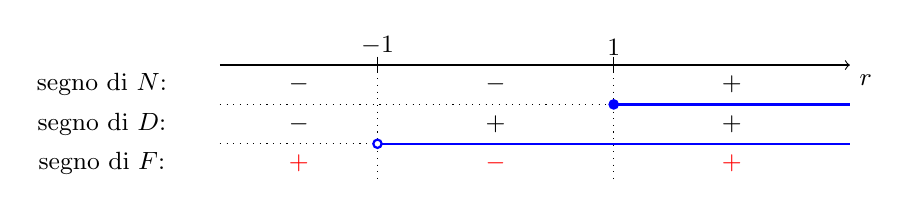
\begin{tikzpicture}[font=\small,x=10mm, y=10mm]

\draw[->] (0,0) -- (8,0) node [below right] () {$r$};

\foreach \x in {2,5}{
\draw(\x,3pt)--(\x,-3pt);
\begin{scope}[dotted]
\draw (\x,0) -- (\x,-1.5);
\draw (0,-.5) -- (5,-.5);
\draw (0,-1) -- (2,-1);
\end{scope}}

\node[above]  at (2,0) {$-1$};
\node[above]  at (5,0) {$1$};

\begin{scope}[blue,thick]
\draw (5,-.5) -- (8,-.5);
\draw (2,-1) -- (8,-1);

\draw[fill=blue] (5,-.5)circle (1.5pt);
\draw[fill=white] (2,-1)circle (1.5pt);
\end{scope}

\foreach \x in {-1.5}{
\node  at (\x,-.25) {segno di $N$:};
\node  at (\x,-.75) {segno di $D$:};
\node  at (\x,-1.25) {segno di $F$:};
}
\foreach \z in {1,3.5}{
\node  at (\z,-.25) {$-$};
}
\foreach \zi in {3.5, 6.5}{
\node  at (\zi,-.75) {$+$};
}

\node  at (6.5,-.25) {$+$};
\node  at (1,-.75) {$-$};

\begin{scope}[red]
\foreach \zii in {1, 6.5}{
\node  at (\zii,-1.25) {$+$};
}
\node  at (3.5,-1.25) {$-$};
\end{scope}
\end{tikzpicture}

\end{center}
Pertanto $\CE\: x<-1\vee x\ge 1$.
\end{esempio}
\end{exrig}

\vspazio\ovalbox{\risolvii \ref{ese:2.11}, \ref{ese:2.12}, \ref{ese:2.13}, \ref{ese:2.14}, \ref{ese:2.15}, \ref{ese:2.16}}

\section{Potenze ad esponente razionale}

In questo paragrafo ci proponiamo di scrivere la radice $n$-esima di un numero reale $a\geq0$ sotto forma di potenza di $a$, vogliamo cioè che sia:
$\sqrt[n]{a}=a^x$.

\paragraph {Caso con esponente positivo}
Elevando ambo i membri dell'uguaglianza alla potenza n otteniamo: $\left(\sqrt[n]a\right)^n=\left(a^x\right)^n$ da cui si ottiene $a=a^{n\cdot x}$.
Trattandosi di due potenze con base~$a{\geq}0$, l'uguaglianza è resa possibile solo se sono uguali gli esponenti. In altre parole, deve essere: $1=n\cdot x \Rightarrow x=\dfrac 1 n$, quindi: $\sqrt[n]a=a^{\frac 1 n}$.

Vediamo ora di generalizzare la formula. Sia $m$ un numero intero positivo, possiamo scrivere $a^{\frac m n}=\left(a^{\frac 1 n}\right)^m$ e quindi $a^{\frac m n}=\left(\sqrt[n]a\right)^m$.
\begin{exrig}
\begin{esempio}
 Calcola le seguenti potenze a esponente razionale positivo.
 \begin{itemize*}
 \item~$27^{\frac 2 3}$: si ha che $27^{\frac 2 3}=\left(\sqrt[3]{27}\right)^2=3^2=9$;
 \item~$25^{\frac 3 2}$: si ha che $25^{\frac 3 2}=\left(\sqrt[2]{25}\right)^3=5^3=125$.
\end{itemize*}
\end{esempio}
\end{exrig}

\paragraph{Caso con esponente negativo}
Per definire la potenza ad esponente razionale negativo è necessario imporre la restrizione $a \neq 0$, infatti risulta:
$a^{-\frac{m}{n}}=\dfrac{1}{a^{\frac{m}{n}}}=\left(\dfrac{1}{a}\right)^{\frac{m}{n}}$

\begin{exrig}
\begin{esempio}
 Calcola le seguenti potenze a esponente razionale negativo.
 \begin{itemize*}
 \item $27^{-\frac{2}{3}}=\dfrac 1{\left(\sqrt[3]{27}\right)^2}=\dfrac 1{3^2}=\dfrac 1 9$;
 \item $125^{-\frac 2 3}=\sqrt[3]{125^{-2}}=\sqrt[3]{(5^3)^{-2}}=\sqrt[3]{(5^{-2})^3}=5^{-2}=\dfrac 1{25}$;
 \item $\left(\dfrac 1 8\right)^{-\frac 3 2}=\sqrt{\left(\dfrac 1 8\right)^{-3}}=\sqrt{8^3}=\sqrt{(2^3)^3}=\sqrt{2^9}$;
 \item $\left(\dfrac 1{49}\right)^{-\frac 1 2}=(49)^{\frac 1 2}=\sqrt{49}=7$.
\end{itemize*}
\end{esempio}
\end{exrig}

In generale si dà la seguente
\begin{definizione}
Si dice \emph{potenza a esponente razionale} $\dfrac{m}{n}$ di un numero reale positivo $a$ l'espressione:
 $a^{\frac{m}{n}}=\sqrt[n]{a^m}=\left(\sqrt[n]{a}\right)^m$ con $\dfrac{m}{n}\in \insQ$.
\end{definizione}

Perché abbiamo dovuto imporre la condizione che $a$ sia un numero positivo?
Partiamo dall'espressione $a^{\frac{1}{n}}$ con $n\in \insN-\{0\}$, se $n$ è dispari la potenza $a^{\frac{1}{n}}$ è sempre definita per ogni valore della base $a$, mentre se è pari $a^{\frac{1}{n}}$ è definita solo per $a\geq 0$.

Nel caso generale, quindi, $a^{\frac{m}{n}}$ con $\dfrac{m}{n}\in \insQ$ la formula $a^{\frac{m}{n}}=\left(\sqrt[n]{a}\right)^m$ è falsa se $a<0$.

Consideriamo il seguente esempio:
 $(-2)^{\frac 6 6}=\left[(-2)^{\frac 1 6}\right]^6=\left(\sqrt[6]{-2}\right)^6$ non è definita nei numeri reali perché non esiste la radice sesta di un numero negativo.
Tuttavia possiamo anche scrivere 
\[(-2)^{\frac 6 6}=\left[(-2)^6\right]^{\frac 1 6}=(64)^{\frac 1 6}=\sqrt[6]{64}=2.\]
Arriviamo pertanto a due risultati differenti.

Per estendere la definizione al caso di basi negative sarebbe necessario stabilire un ordine di priorità delle operazioni ma ciò andrebbe contro la proprietà commutativa del prodotto degli esponenti di una potenza di potenza.

\vspazio\ovalbox{\risolvii \ref{ese:2.17}, \ref{ese:2.18}, \ref{ese:2.19}, \ref{ese:2.20}, \ref{ese:2.21}}

\section{Semplificazione di radici}

\begin{proposizione}
Il valore di una radice in $\insR^+\cup \{0\}$ non cambia se moltiplichiamo l'indice della radice e l'esponente del radicando per uno stesso numero intero positivo. In simboli $\sqrt[n]{a^m}=\sqrt[nt]{a^{mt}}$ con $a\ge 0$ e $m$, $n$, $t\in \insN-\{0\}$.
\end{proposizione}
\pagebreak
\begin{exrig}
 \begin{esempio}
 Radici equivalenti.
 \begin{itemize}
 \item $\sqrt{2}=\sqrt[4]{2^2}$: abbiamo moltiplicato per $2$ indice della radice ed esponente del radicando;
 \item $\sqrt[3]{a}=\sqrt[9]{a^3}$: abbiamo moltiplicato per $3$ indice della radice ed esponente del radicando.
\end{itemize}
 \end{esempio}
\end{exrig}

\begin{proposizione}
Il valore di una radice in $\insR^{+}\cup \{0\}$ non cambia se dividiamo l'indice della radice e l'esponente del radicando per un loro divisore comune. In simboli $\sqrt[nt]{a^{mt}}=\sqrt[n]{a^m}$ con $a\ge 0$ e $m$, $n$, $t\in \insN-\{0\}$.
\end{proposizione}

\begin{exrig}
 \begin{esempio}
Semplificazione di radici
\begin{itemize}
 \item $\sqrt[4]{2^2}=\sqrt 2$: abbiamo semplificato per $2$ indice della radice ed esponente del radicando;
 \item $\sqrt[10]{3^{15}}=\sqrt{3^3}$: abbiamo semplificato per $5$;
 \item $\sqrt[7]{3^9}$: non è riducibile perché indice della radice ed esponente non hanno divisori comuni;
 \item $\sqrt[8]{2^6}=2^{\frac 6 8}$: semplificando la frazione dell'esponente otteniamo $2^{\frac 3 4}=\sqrt[4]{2^3}$;
 \item $\sqrt[6]{\left(\dfrac 1 5\right)^{-9}}=\sqrt[6]{5^9}=\sqrt[2]{5^3}$;
 \item $\sqrt[4]{(-3)^2}=\sqrt[4]{3^2}=\sqrt 3$;
 \item $\sqrt{10^{-4}}$: semplificando per $2$ indice della radice ed esponente del radicando si ottiene~$10^{-2}=\dfrac 1{100}$;
 \item $\sqrt{30\cdot 27\cdot 10}$: scomponendo in fattori primi otteniamo \[\sqrt{30\cdot 27\cdot 10}=\sqrt{2\cdot 3\cdot 5\cdot 3^3\cdot 2\cdot 5}=\sqrt{2^2\cdot 3^4\cdot 5^2}.\] Osserviamo che tutti gli esponenti del radicando e l'indice della radice hanno in comune il divisore 2, quindi $\sqrt{2^2\cdot 3^4\cdot 5^2}=2\cdot 3^2\cdot 5=90.$
\end{itemize}
\end{esempio}
\end{exrig}

Se il radicando è un'espressione letterale, quindi è possibile che sia positiva che negativa, dobbiamo scrivere
\[
\sqrt[nt]{a^{mt}}=
\begin{cases}
\sqrt[n]{a^m} & \text{ se }t\text{ è dispari}\\
\sqrt[n]{\left|a^m\right|} & \text{ se }t\text{ è pari}
\end{cases}.
\]

\begin{exrig}
 \begin{esempio}
Semplificazione di radici con espressione letterale come radicando.
\begin{itemize}
\item $\sqrt{4x^4y^2a^6}=\sqrt{2^2x^4y^2a^6}=2x^2\left|ya^3\right|$: abbiamo semplificato per $2$ sia l'indice della radice che l'esponente del radicando;
\item $\sqrt[12]{a^2+2a+1}=\sqrt[12]{(a+1)^2}=\sqrt[6]{\left|a+1\right|}$: dopo aver riconosciuto che il radicando è il quadrato del binomio, abbiamo semplificato per $2$ indice ed esponente;
\item $\sqrt{x^2y^2}=\valass{xy}$;
\item $\sqrt{x^2+2xy+y^2}=\sqrt{(x+y)^2}=\valass{x+y}$;
\item $\sqrt{x^2+y^2}$ non è semplificabile perché il radicando non può essere espresso sotto forma di potenza;
\item $\sqrt[6]{(x-1)^2}=\sqrt[3]{\valass{x-1}}$;
\end{itemize}
 \end{esempio}
\end{exrig}

La proprietà invariantiva si può applicare per semplificare i radicali se la base del radicando è positiva o nulla, se fosse negativa si potrebbe perdere la concordanza del segno. Per esempio~$\sqrt[10]{(-2)^6}\neq \sqrt[5]{(-2)^3}$, infatti il primo radicando è positivo mentre il secondo è negativo.

Invece $\sqrt[9]{(-2)^3}=\sqrt[3]{-2}$ perché in questo caso la concordanza del segno è conservata, infatti pur essendo la base negativa, l'esponente resta dispari, conservando il segno della base.

Se il radicando ha base negativa e nella semplificazione il suo esponente passa da pari a dispari è necessario mettere il radicando in valore assoluto: $\sqrt[10]{(-2)^6}=\sqrt[5]{\left|-2^3\right|}$.

Se il radicando è letterale si segue la stessa procedura: ogni volta che studiando il segno del radicando si trova che la base può essere negativa, se l'esponente del radicando passa da pari a dispari, si mette il modulo per garantire la concordanza del segno:
$\sqrt[10]{x^6}=\sqrt[5]{\left|x^3\right|}$, $\CE\: \forall x \in \insR$.

\vspazio\ovalbox{\risolvii \ref{ese:2.22}, \ref{ese:2.23}, \ref{ese:2.24}, \ref{ese:2.25}, \ref{ese:2.26}, \ref{ese:2.27}, \ref{ese:2.28}, \ref{ese:2.29}, \ref{ese:2.30}, \ref{ese:2.31}, \ref{ese:2.32}, \ref{ese:2.33}, \ref{ese:2.34}}

\section{Moltiplicazione e divisione di radici}
Prima di operare con i radicali letterali, è necessario determinare le condizioni di esistenza: il prodotto di due radicali esiste là dove sono soddisfatte le condizioni di esistenza di tutti i fattori; il quoziente esiste là dove sono soddisfatte le condizioni di esistenza di dividendo e divisore, con il divisore diverso da zero.

\subsection{Moltiplicazione e divisione di radici con lo stesso radicando}
Per effettuare la moltiplicazione o la divisione tra radici aventi lo stesso radicando si possono trasformare le radici in forma di potenze con esponente razionale e utilizzare le proprietà delle potenze.

\begin{exrig}
 \begin{esempio}
Moltiplicazione e divisione di radici con lo stesso radicando.
\begin{itemize}
\item $\sqrt[4]6\cdot \sqrt[3]6=6^{\frac 1 4}\cdot 6^{\frac 1 3}=6^{\frac 1 4+\frac 1 3}=6^{\frac 7{12}}=\sqrt[12]{6^7}$;
\item $\sqrt[4]6:\sqrt[3]6=6^{\frac 1 4}:6^{\frac 1 3}=6^{\frac 1 4-\frac 1 3}=6^{-\frac 1{12}}=\dfrac 1{\sqrt[12]6}$.
\end{itemize}
 \end{esempio}
\end{exrig}

\subsection{Moltiplicazione e divisione di radici con lo stesso indice}
Il prodotto di due radici che hanno lo stesso indice è una radice che ha per indice lo stesso indice e per radicando il prodotto dei radicandi:
\[\sqrt[n]a\cdot \sqrt[n]b=\sqrt[n]{ab}.\]

Allo stesso modo, il quoziente di due radici che hanno lo stesso indice è una radice che ha per indice lo stesso indice e \ per radicando il quoziente dei radicandi:
\[\sqrt[n]a:\sqrt[n]b=\sqrt[n]{a:b} \Rightarrow \dfrac{\sqrt[n]a}{\sqrt[n]b}=\sqrt[n]{\dfrac a b}.\]

Per rendersi conto di questa proprietà si possono trasformare le radici in potenze ad esponenti razionali e applicare le proprietà delle potenze:
 \[\sqrt[n]a\cdot \sqrt[n]b=a^{\frac 1 n}\cdot b^{\frac 1 n}=(ab)^{\frac 1 n}=\sqrt[n]{ab}\text{,}\quad \sqrt[n]a:\sqrt[n]b=a^{\frac 1 n}:b^{\frac 1 n}=\left(\dfrac a b\right)^{\frac 1 n}=\sqrt[n]{\dfrac a b}.\]

\begin{exrig}
 \begin{esempio}
Moltiplicazione e divisione di radici con lo stesso indice.
\begin{itemize}
\item $\sqrt 2\cdot \sqrt 3=\sqrt{2\cdot 3}=\sqrt 6$;
\item $\frac{\sqrt[3]9}{\sqrt[3]{72}}=\sqrt[3]{\frac 9{72}}=\sqrt[3]{\frac 1 8}=\frac 1 2$;
\item $\sqrt{2a}\cdot \sqrt{\frac a b}:\sqrt{\frac {2b} 9}$,\, $\CE a\ge 0\wedge b>0$\, $\sqrt{2a}\cdot \sqrt{\frac a b}:\sqrt{\frac {2b} 9}=\sqrt{2a\cdot \frac a b\cdot \frac 9{2b}}=\sqrt{\frac{9a^2}{b^2}}=\frac {3a} b$.
\end{itemize}
 \end{esempio}
\end{exrig}

\subsection{Moltiplicazione e divisione di radici con indici diversi}
Per moltiplicare o dividere radici con indici differenti è necessario prima ridurre le radici allo stesso indice, cioè trasformarle in radici equivalenti con lo stesso indice usando la proprietà invariantiva. Dopo aver ottenuto radici con lo stesso indice si applica la regola precedente.

\begin{procedura}
Ridurre due o più radici allo stesso indice:
\begin{enumeratea}
 \item scomporre in fattori irriducibili tutti i radicandi;
 \item porre le condizioni di esistenza;
 \item calcolare il minimo comune multiplo tra gli indici delle radici;
 \item per ciascuna radice dividere il~$\mcm$ per l'indice della radice e moltiplicare il quoziente trovato per l'esponente del radicando.
\end{enumeratea}
\end{procedura}

\begin{exrig}
 \begin{esempio}
Moltiplicazione e divisione di radici con indice diverso.
\begin{itemize}
\item $\sqrt 2\cdot \sqrt[3]2=\sqrt[6]{2^3}\cdot \sqrt[6]{2^2}=\sqrt[6]{2^3\cdot 2^2}=\sqrt[6]{2^5}$. Gli indici delle radici sono $2$ e $3$, il loro~$\mcm$ è~$6$, il primo radicando va elevato a~$6:2$ cioè~$3$, mentre il secondo radicando va elevato a~$6:3$ cioè~$2$;
\item $\sqrt[3]{\frac 3 2}\cdot \sqrt[4]{\frac 8{27}}:\sqrt[6]{\frac 2 3}=\sqrt[12]{\frac{3^4}{2^4}\cdot \frac{8^3}{27^3}:\frac{2^2}{3^2}}=\sqrt[12]{\frac{3^4}{2^4}\cdot \frac{2^9}{3^9}:\frac{2^2}{3^2}}=\sqrt[12]{\frac{3^6\cdot 2^9}{3^9\cdot 2^6}}=\sqrt[12]{\frac{2^3}{3^3}}=\sqrt[4]{\frac 2 3}$. Il $\mcm$ tra gli indici delle radici è $12$. Il primo radicando va elevato a $12:3=4$, il secondo radicando va elevato a $12:4=3$ e il terzo va elevato a $12:6=2$.
\end{itemize}
 \end{esempio}

\begin{esempio}
 $\dfrac{\sqrt[3]{x^2y}\cdot \sqrt{xy}}{\sqrt[6]{x^2y^3}}$, $\CE\: x>0\wedge y>0$.
Il $\mcm$ degli indici delle radici è $6$, quindi:
\[
\frac{\sqrt[3]{x^2y}\cdot \sqrt{\mathit{xy}}}{\sqrt[6]{x^2y^3}}=\sqrt[6]{\frac{\left(x^2y\right)^2\cdot (xy)^3}{x^2y^3}}=\sqrt[6]{\frac{x^4y^2x^3y^3}{x^2y^3}}=\sqrt[6]{\frac{x^7y^5}{x^2y^3}}=\sqrt[6]{x^5y^2}.
\]
\end{esempio}

\begin{esempio}
 $\sqrt[3]{\dfrac{ax+a}{x^2+2x+1}}\cdot \sqrt{\dfrac{x^2-2x+1}{ax-a}}$.
\begin{enumeratea}
\item Scomponiamo in fattori i radicandi $\sqrt[3]{\dfrac{a(x+1)}{(x+1)^2}}\cdot \sqrt{\dfrac{(x-1)^2}{a(x-1)}}$;
\item $\CE\: x+1\neq 0\wedge a(x-1)>0\:\Rightarrow\: x\neq -1\wedge ((a>0\wedge x>1)\vee (a<0\wedge x<1))$;
\item Semplifichiamo le frazioni di ciascun radicando $\sqrt[3]{\dfrac a{x+1}}\cdot \sqrt{\dfrac{x-1} a}$;
\item Trasformiamo nello stesso indice: il~$\mcm$ degli indici è~$6$, quindi:
\[
\sqrt[6]{\left(\dfrac a{x+1}\right)^2}\cdot \sqrt[6]{\left(\dfrac{x-1} a\right)^3}=\sqrt[6]{\dfrac{a^2}{(x+1)^2}\cdot \dfrac{(x-1)^3}{a^3}}=\sqrt[6]{\dfrac{(x-1)^3}{a(x+1)^2}}
\]
\end{enumeratea}
\end{esempio}

\begin{esempio}
 $\sqrt[3]{\dfrac{x^2}{x^2-2x+1}}:\sqrt[4]{\dfrac{x^4-2x^2+1}{x^2-1}}$.
\begin{enumeratea}
\item Scomponiamo in fattori i radicandi $\sqrt[3]{\dfrac{x^2}{(x-1)^2}}:\sqrt[4]{\dfrac{(x-1)^2\cdot (x+1)^2}{(x+1)(x-1)}}$;
\item $\CE\:(x-1)(x+1)>0\:\Rightarrow\: x<-1\vee x>1$. L'operazione che dobbiamo eseguire è una divisione e dunque il divisore deve essere diverso da zero, quindi $x\neq -1\wedge x\neq 1$, comunque già implicite nelle $\CE$ trovate;
\begin{center}
 % (c) 2013 Claudio Carboncini - claudio.carboncini@gmail.com
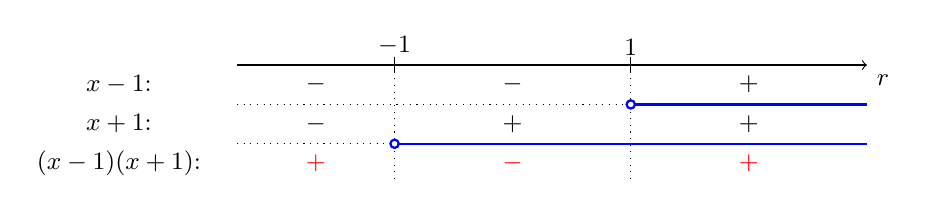
\begin{tikzpicture}[font=\small,x=10mm, y=10mm]

\draw[->] (0,0) -- (8,0) node [below right] () {$r$};

\foreach \x in {2,5}{
\draw(\x,3pt)--(\x,-3pt);
\begin{scope}[dotted]
\draw (\x,0) -- (\x,-1.5);
\draw (0,-.5) -- (5,-.5);
\draw (0,-1) -- (2,-1);
\end{scope}}

\node[above]  at (2,0) {$-1$};
\node[above]  at (5,0) {$1$};

\begin{scope}[blue,thick]
\draw (5,-.5) -- (8,-.5);
\draw (2,-1) -- (8,-1);

\draw[fill=white] (5,-.5)circle (1.5pt);
\draw[fill=white] (2,-1)circle (1.5pt);
\end{scope}

\foreach \x in {-1.5}{
\node  at (\x,-.25) {$x-1$:};
\node  at (\x,-.75) {$x+1$:};
\node  at (\x,-1.25) {$(x-1)(x+1)$:};
}
\foreach \z in {1,3.5}{
\node  at (\z,-.25) {$-$};
}
\foreach \zi in {3.5, 6.5}{
\node  at (\zi,-.75) {$+$};
}

\node  at (6.5,-.25) {$+$};
\node  at (1,-.75) {$-$};

\begin{scope}[red]
\foreach \zii in {1, 6.5}{
\node  at (\zii,-1.25) {$+$};
}
\node  at (3.5,-1.25) {$-$};
\end{scope}
\end{tikzpicture}

\end{center}
\item Semplifichiamo i radicandi $\sqrt[3]{\dfrac{x^2}{(x-1)^2}}:\sqrt[4]{(x-1)\cdot (x+1)}$;
\item Riduciamo allo stesso indice: il $\mcm$ degli indici è $12$, quindi:

$\sqrt[12]{\left[\frac{x^2}{(x-1)^2}\right]^4}:\sqrt[12]{(x-1)^3 (x+1)^3}\Rightarrow \sqrt[12]{\frac{x^8}{(x-1)^8}\cdot \frac 1{(x-1)^3 (x+1)^3}}=\sqrt[12]{\frac{x^8}{(x-1)^{11}(x+1)^3}}$.
\end{enumeratea}
\end{esempio}
\end{exrig}

\vspazio\ovalbox{\risolvii \ref{ese:2.35}, \ref{ese:2.36}, \ref{ese:2.37}, \ref{ese:2.38}, \ref{ese:2.39}, \ref{ese:2.40}, \ref{ese:2.41}, \ref{ese:2.42}, \ref{ese:2.43}, \ref{ese:2.44}, \ref{ese:2.45}, \ref{ese:2.46}, \ref{ese:2.47}}

\section{Portare un fattore sotto il segno di radice}
Per portare un fattore dentro il segno di radice bisogna elevarlo all'indice della radice:
\[
a\sqrt[n]b=
\begin{cases}
\sqrt[n]{a^n\cdot b} & \text{ se }n\text{ è pari e }a\ge 0\\
-\sqrt[n]{a^n\cdot b} & \text{ se }n\text{ è pari e }a<0\\
\sqrt[n]{a^n\cdot b} & \text{ se }n\text{ è dispari}
\end{cases}.
\]

%\begin{itemize*}
% \item $a\sqrt[n]b=\sqrt[n]{a^n\cdot b}$ se $n$ è pari e $a\ge 0$;
% \item $a\sqrt[n]b=-\sqrt[n]{a^n\cdot b}$ se $n$ è pari e $a<0$;
% \item $a\sqrt[n]b=\sqrt[n]{a^n\cdot b}$ se $n$ è dispari.
%\end{itemize*}

Ricordando che abbiamo posto $\sqrt[1]a=a$, portare un fattore sotto radice quivale a svolgere la moltiplicazione tra una radice di indice $1$ e una radice di indice $n$ qualsiasi.
\begin{exrig}
 \begin{esempio}
 Portare un numero reale dentro il segno di radice.
 \begin{itemize}
 \item $2\cdot \sqrt[3]7=\sqrt[3]{2^3\cdot 7}=\sqrt[3]{56}$;
 \item $3\cdot \sqrt{\frac 2{21}}=\sqrt{3^2\cdot \frac 2{21}}=\sqrt{9\cdot \frac 2{21}}=\sqrt{\frac 6 7}$;
 \item $-\frac 1 2\sqrt 3\:$ (lasciamo il segno ``$-$'' fuori dalla radice) $\:\Rightarrow\:-\frac 1 2\sqrt 3=-\sqrt{\left(\frac 1 2\right)^2\cdot 3}=-\sqrt{\frac 3 4}$;
 \item $-\frac 1 3\cdot \sqrt{12}=-\sqrt{\left(\frac 1 3\right)^2\cdot 12}=-\sqrt{\frac 1 9\cdot 12}=-\sqrt{\frac 4 3}$;
 \item $\left(1-\sqrt 2\right)\cdot \sqrt 3=-	\left(\sqrt 2-1\right)\cdot \sqrt 3=-\sqrt{(\sqrt 2-1)^2\cdot 3}$;
 \item $-2\sqrt[3]5=\sqrt[3]{(-2)^3\cdot 5}=\sqrt[3]{-40}$.
 \end{itemize}
 \end{esempio}

 \begin{esempio}
 Portare una espressione letterale dentro il segno di radice.
 \begin{itemize}
 \item $a\cdot \sqrt[3]b=\sqrt[3]{a^3b}\:$ l'indice della radice è dispari pertanto $a$ si porta sotto radice senza alcuna condizione;
 \item $(x-1)\cdot \sqrt[3]x=\sqrt[3]{(x-1)^3\cdot x}\:$ l'indice della radice è dispari, non sono necessarie condizioni sulla $x$;
 \item $(x-2)\sqrt y\:$ osserviamo che il radicale (indice 2, pari) esiste per $y\ge 0$.
 Per portare dentro il segno di radice il coefficiente $(x-2)$ bisogna fare la distinzione:
 \[
 (x-2)\sqrt y=
 \begin{cases}
 \sqrt{(x-2)^2y} & \text{ se }x\ge 2\\
 -(2-x)\sqrt y=-\sqrt{(2-x)^2y} & \text{ se }x<2
 \end{cases};
 \]
 \item $(x-1)\sqrt{x-2}\:$ il radicale esiste per $x-2\ge 0\ \:\Rightarrow\: \ x\ge 2$, per questi valori $(x-1)\ge 0$ e può essere portato dentro la radice: \[(x-1)\sqrt{x-2}=\sqrt{(x-1)^2(x-2)};\]
 \item $\dfrac{a-1}{a+3}\cdot \sqrt{\dfrac{a+2}{(a-1)^2}}$. Determiniamo le condizioni di esistenza del radicale: per l'esistenza della frazione $\dfrac{a+2}{(a-1)^2}$ deve essere $(a-1)^2\neq 0$, ovvero $a\neq 1$. Affinché il radicando sia positivo o nullo, essendo il denominatore sempre positivo (ovviamente per $a\neq 1$) è sufficiente che sia $a+2\geqslant 0$ ovvero $a\geqslant -2$. Pertanto le condizioni di esistenza sono~ $a\geqslant -2$ e $a\neq 1$.

 Studiamo ora il segno della frazione algebrica da portare sotto radice: tale frazione è positiva o nulla per $a<-3\vee a\geqslant 1$, è negativa per $-3<a\leqslant 1$.

 Se $a>1$ si ha $\dfrac{a-1}{a+3}\cdot \sqrt{\dfrac{a+2}{(a-1)^2}}=\sqrt{\dfrac{(a-1)^2}{(a+3)^2}\cdot \dfrac{a+2}{(a-1)^2}}=\sqrt{\dfrac{a+2}{(a+3)^2}}$.

 Se $-2<a<1$ il fattore da portare sotto radice è negativo, quindi:
 \[-\left(-\frac{a-1}{a+3}\right)\cdot \sqrt{\frac{a+2}{(a-1)^2}}=-\sqrt{\frac{[-(a-1)]^2}{(a+3)^2}\cdot \frac{a+2}{(a-1)^2}}=-\sqrt{\frac{a+2}{(a+3)^2}}.\]

 Se $a=-2$ l'espressione vale zero.
 
 Il caso $a=1$ è comunque escluso dalla condizione di esistenza.
 \end{itemize}
 \end{esempio}
\end{exrig}
\vspazio\ovalbox{\risolvii \ref{ese:2.48}, \ref{ese:2.49}, \ref{ese:2.50}, \ref{ese:2.51}}

\section{Portare un fattore fuori dal segno di radice}

È possibile portare fuori dal segno di radice quei fattori aventi come esponente un numero che sia maggiore o uguale all'indice della radice. In generale si inizia scomponendo in fattori irriducibili il radicando, ottenendo un radicale del tipo $\sqrt[n]{a^m}$ con $m\ge n$.

\paragraph{I° modo:} si esegue la divisione intera $m:n$ ottenendo un quoziente $q$ e un resto $r$. Per la proprietà della divisione si ha $\;m=n\cdot q+r\;$ quindi $\sqrt[n]{a^m}=\sqrt[n]{a^{n\cdot q+r}}$ e per le proprietà delle potenze $\sqrt[n]{a^{n\cdot q+r}}=\sqrt[n]{(a^q)^n\cdot a^r}$ e per la regola del prodotto di due radici con medesimo indice si ottiene:
\[\sqrt[n]{a^{n\cdot q+r}}=\sqrt[n]{(a^q)^n\cdot a^r}=\sqrt[n]{(a^q)^n}\cdot \sqrt[n]{a^r}=a^q\cdot \sqrt[n]{a^r}\:\text{ con } r<n.\]
Notiamo che il fattore “fuori“ dalla radice ha per esponente il quoziente della divisione intera, mentre il fattore che rimane “dentro“ ha per esponente il resto della divisione stessa.

 $\sqrt[3]{a^8}=\ldots\:$ eseguiamo la divisione $8:3$ con $q=2$ e $r=2$, quindi $\sqrt[3]{a^8}=a^2\cdot \sqrt[3]{a^2}$.

\paragraph{II° modo:} si può trasformare la potenza del radicando nel prodotto di due potenze con la stessa base; una avente esponente multiplo dell'indice della radice e l'altra avente per esponente la differenza tra l'esponente iniziale e il multiplo trovato. Consideriamo il seguente esempio:

 $\sqrt[3]{a^8}=\ldots\:$ il multiplo di $3$ più vicino a $8$ è $6$, quindi 
\[\sqrt[3]{a^8}=\sqrt[3]{a^6\cdot a^2}=\sqrt[3]{a^6}\cdot \sqrt[3]{a^2}=a^2\cdot \sqrt[3]{a^2}.\]
\pagebreak
\begin{exrig}
 \begin{esempio}
 Portare un numero reale fuori dal segno di radice.
\begin{itemize}
 \item $\sqrt{\np{1200}}$ Si scompone in fattori primi il radicando $\np{1200}=2^4\cdot 5^2\cdot 3$ ne segue allora che $\sqrt{\np{1200}}=\sqrt{2^4\cdot 5^2\cdot 3}=2^2\cdot 5\sqrt 3=20\sqrt 3$;
 \item $\sqrt{75}=\sqrt{5^2\cdot 3}=5\sqrt 3$;
 \item $\sqrt{720}=\sqrt{2^4\cdot 3^2\cdot 5}=2^2\cdot 3\cdot \sqrt 5=12\sqrt 5$.
\end{itemize}
 \end{esempio}
\end{exrig}

Quando portiamo fuori dalla radice un termine letterale dobbiamo verificare se l'indice della radice è pari o dispari e se il termine che portiamo fuori è positivo o negativo. In particolare:
\[
\sqrt[n]{a^nb}=
\begin{cases}
a\sqrt[n]b & \text{ se }n\text{ è dispari}\\
\valass a\sqrt[n]b & \text{ se }n\text{ è pari}
\end{cases}.
\]

\begin{exrig}
 \begin{esempio}
 Portare una espressione letterale fuori dal segno di radice.
\begin{itemize}
 \item $\sqrt{2a^2}=\valass a\sqrt 2$: bisogna mettere $a$ in valore assoluto perché sotto radice poteva essere sia negativo che positivo, la radice (di indice 2, pari) invece deve essere sempre positiva; se $a<0$ la relazione~$\sqrt{2a^2}=a\sqrt 2$ è errata;
 \item $\sqrt[3]{a^5b^7cd^3}$ occorre eseguire le divisioni intere tra gli esponenti e l'indice della radice. Cominciamo da $a^5$ risulta $5:3 = 1$ con resto uguale a $2$; per $b^7$ si ha $7:3$ con quoziente~$2$ e resto~$1$; l'esponente di $c$ è minore dell'indice; per $d^3$ si ha $3:3$ con quoziente $1$ e resto~$0$. In definitiva $\sqrt[3]{a^5b^7cd^3}={ab}^2 d\sqrt[3]{a^2{bc}}$, o anche:
\[\sqrt[3]{a^5b^7cd^3}=\sqrt[3]{(a^3a^2)(b^6b)cd^3}=\sqrt[3]{a^3b^6d^3}\cdot \sqrt[3]{a^2bc}=ab^2d^3\sqrt[3]{a^2bc}.\]
In questo caso non c'è da mettere il valore assoluto perché l'indice della radice è dispari;
 \item $\sqrt[3]{\dfrac{3^3x^3y}{z^6}}=3\dfrac x{z^2}\sqrt[3]y$, $\:\CE\: z\neq 0$;
 \item$\sqrt[4]{4x^4-4x^5}$ scomponiamo il radicando per poter studiare le condizioni di esistenza del radicale e portare fuori qualche fattore: 
 \[\sqrt[4]{4x^4-4x^5}=\sqrt[4]{4x^4(1-x)}\quad \CE\: 1-x\ge 0\:\Rightarrow\: x\le 1.\]
 Pertanto:
 \[\sqrt[4]{4x^4-4x^5}=\sqrt[4]{4x^4(1-x)}=\valass x\sqrt[4]{4(1-x)}=
 \begin{cases}
 x\sqrt[4]{4(1-x)} & \text{ se }0\le x\le 1\\
 -x\sqrt[4]{4(1-x)} & \text{ se }x<0
 \end{cases};\]
 \item $\sqrt{3(a-1)^2}=\valass{a-1}\sqrt 3=
 \begin{cases}
 (a-1)\sqrt 3 & \text{ se }a>1\\
 0 & \text{ se }a=1\\
 (1-a)\sqrt 3 & \text{ se }a<1
 \end{cases}$.
\end{itemize}
 \end{esempio}
\end{exrig}
\vspazio\ovalbox{\risolvii \ref{ese:2.52} \ref{ese:2.53}, \ref{ese:2.54}, \ref{ese:2.55}, \ref{ese:2.56}, \ref{ese:2.57}}

\section{Potenza di radice e radice di radice}

Per elevare a potenza una radice si eleva a quella potenza il radicando: $\left(\sqrt[n]a\right)^m=\sqrt[n]{a^m}$.
Si capisce il perché di questa proprietà trasformando, come negli altri casi, la radice in potenza con esponente frazionario:
$\left(\sqrt[n]a\right)^m=\left(a^{\frac 1 n}\right)^m=a^{\frac m n}=\sqrt[n]{a^m}$.
%\newpage
\begin{exrig}
 \begin{esempio}
 Potenza di radice.
 \begin{multicols}{2}
 \begin{itemize}
 \item $\left(\sqrt 2\right)^2=\sqrt{2^2}=2$;
 \item $\left(\sqrt[3]{2ab^2c^3}\right)^2=\sqrt[3]{4a^2b^4c^6}$.
 \end{itemize}
 \end{multicols}
 \end{esempio}
\end{exrig}

La radice di un'altra radice è uguale a una radice con lo stesso radicando e con indice il prodotto degli indici delle radici: $\sqrt[m]{\sqrt[n]a}=\sqrt[m\cdot n]a$. Anche questa proprietà si può spiegare con le proprietà delle potenze trasformando la radice in potenza con esponente frazionario: $\sqrt[m]{\sqrt[n]a}=\left(a^{\frac 1 n}\right)^{\frac 1 m}=a^{\frac 1{mn}}=\sqrt[m\cdot n]a$
\begin{exrig}
 \begin{esempio}
 Radice di radice.
 \begin{multicols}{2}
 \begin{itemize}
 \item $\sqrt{\sqrt 2}=\sqrt[2\cdot 2]2=\sqrt[4]2$;
 \item $\sqrt[3]{\sqrt[4]{2x}}=\sqrt[12]{2x}$.
 \end{itemize}
 \end{multicols}
 \end{esempio}

 \begin{esempio}
 Data l'espressione $\sqrt[5]{3\cdot\sqrt{2}}$ ridurla ad unico radicale.

 In questo caso non possiamo subito applicare la regola annunciata, ma dobbiamo portare il fattore esterno dentro la radice più interna ottenendo $\sqrt[5]{\sqrt{3^2 \cdot 2}}=\sqrt[10]{18}$.

 Osserviamo che in genere l'espressione $\sqrt[n]{a+\sqrt{b}}$ non si può ridurre ad unico radicale, se non sotto determinate condizioni che analizzeremo in seguito.
 \end{esempio}
\end{exrig}
\vspazio\ovalbox{\risolvii \ref{ese:2.58}, \ref{ese:2.59}, \ref{ese:2.60}, \ref{ese:2.61}, \ref{ese:2.62}}

\section{Somma di radicali}

\begin{definizione}
Si dice \emph{radicale} un'espressione del tipo $a\sqrt[n]b$ con $a$ e $b$ numeri reali, $b{\geq}0$ ed $n\in \insN$. Il numero $a$ prende il nome di \emph{coefficiente} del radicale.
\end{definizione}

Operare con i radicali è simile al modo di operare con i monomi. Infatti è possibile effettuare somme algebriche soltanto se i radicali hanno lo stesso indice e lo stesso radicando, mentre si possono sempre effettuare moltiplicazioni e divisioni dopo averli ridotti allo stesso indice.
\begin{definizione}
 Due radicali si dicono \emph{simili} se hanno lo stesso indice e lo stesso radicando.
\end{definizione}

\`E possibile effettuare somme algebriche soltanto se i radicali sono simili, si eseguono le somme allo stesso modo in cui si eseguono le somme algebriche dei monomi.

Attenzione, l'operazione $\sqrt 2+\sqrt 3=\sqrt 5$\, è errata in quanto i radicali addendi non sono simili poiché hanno lo stesso indice (2) ma non lo stesso radicando.
\pagebreak
\begin{exrig}
 \begin{esempio}
Esegui le seguenti somme di radicali.
\begin{itemize}
 \item $\sqrt 8+\sqrt 2=\sqrt{2^3}+\sqrt 2=2\sqrt 2+\sqrt 2=3\sqrt 2$;
 \item $2\sqrt{45}-\sqrt{80}=2\sqrt{3^2\cdot 5}-\sqrt{2^4\cdot 5}=2\cdot 3\cdot \sqrt 5-2^2\sqrt 5=6\sqrt 5-4\sqrt 5=2\sqrt 5$;
 \item $\sqrt 2+\sqrt 3$\, non si può eseguire perché i radicali non sono simili;
 \item $\sqrt[3]2+\sqrt 2$\, non si può eseguire perché i radicali non sono simili;
 \item $\sqrt 3+\sqrt 3=2\sqrt 3$;
 \item $2\sqrt 5-\sqrt 5=\sqrt 5$;
 \item $\frac 1 2\sqrt 7-\frac 4 3\sqrt 7=\left(\frac 1 2-\frac 4 3\right)\sqrt 7=\frac{3-8} 6\sqrt 7=-\frac 5 6\sqrt 7$;
 \item $3\sqrt 2+2\sqrt 3-2\sqrt 2+3\sqrt 3=(3-2)\sqrt 2+(2+3)\sqrt 3=\sqrt 2+5\sqrt 3$\, abbiamo sommato i radicali simili;
 \item $2\sqrt a+3\sqrt a=5\sqrt a$, $\CE\: a\ge 0$;
 \item $\sqrt[4]{a^5}+\sqrt[4]{a^3}\cdot \sqrt a+\sqrt[4]{a^6}:\sqrt[4]a$. Poniamo le condizioni di esistenza ($a>0$) e svolgiamo i calcoli: $\sqrt[4]{a^5}+\sqrt[4]{a^3\cdot a^2}+\sqrt[4]{a^6:a}=\sqrt[4]{a^5}+\sqrt[4]{a^5}+\sqrt[4]{a^5}=3\sqrt[4]{a^5}=3\sqrt[4]{a^4\cdot a}=3a\sqrt[4]a$.
\end{itemize}
 \end{esempio}
\end{exrig}
Per semplificare le espressioni che seguono, useremo le procedure di calcolo dei polinomi.
\begin{exrig}
 \begin{esempio}
Esegui le seguenti operazioni con i radicali.
\begin{itemize}
 \item $(1+\sqrt 2)(3\sqrt 2-1)=3\sqrt 2-1+3\sqrt {2^2}-\sqrt 2=3\sqrt 2-1+3\cdot 2-\sqrt 2=2\sqrt 2+5$;
 \item $(\sqrt 3+1)^2=(\sqrt 3)^2+(1)^2+2\cdot \sqrt 3\cdot 1=3+1+2\sqrt 3=4+2\sqrt 3$;
 \item $(\sqrt 3-\sqrt 2)^2=(\sqrt 3)^2+(\sqrt 2)^2+2 \sqrt 3 (-\sqrt 2)=3+2-2\sqrt 6=5-2\sqrt 6$;
 \item $(3+\sqrt 2+\sqrt 3)^2=(3)^2+(\sqrt 2)^2+(\sqrt 3)^2+6 \sqrt 2+6 \sqrt 3+2 \sqrt 2 \sqrt 3=14+6\sqrt 2+6\sqrt 3+2\sqrt 6$;
 \item $(\sqrt 2+4)(3-\sqrt 2)=3\sqrt 2 +\sqrt 2(-\sqrt 2)+12+4(-\sqrt 2)=3\sqrt 2-2+12-4\sqrt 2=10-\sqrt 2$;
 \item $(\sqrt 2-3)^3=(\sqrt 2)^3-9(\sqrt 2)^2+27\sqrt 2+(-3)^3=2\sqrt 2-18+27\sqrt 2-27=29\sqrt 2-45$.
\end{itemize}
 \end{esempio}
\end{exrig}
Le espressioni con radicali possono essere trasformate in potenze con esponente frazionario per poi applicare le proprietà delle potenze:
\begin{exrig}
 \begin{esempio}
Trasforma i radicali in potenze con esponente frazionario applicando le proprietà delle potenze.
\begin{itemize}
 \item $\dfrac{\sqrt a\cdot \sqrt[3]{a^2\cdot b}}{\sqrt[6]{a^5\cdot b}}$.
 \[\dfrac{\sqrt a\cdot \sqrt[3]{a^2\cdot b}}{\sqrt[6]{a^5\cdot b}}=\dfrac{a^{\frac 1 2}\cdot a^{\frac 2 3}\cdot b^{\frac 1 3}}{a^{\frac 5 6}\cdot b^{\frac 1 6}}=a^{\frac 1 2+\frac 2 3-\frac 5 6}\cdot b^{\frac 1 3-\frac 1 6}=a^{\frac 2 6}\cdot b^{\frac 1 6}=\sqrt[6]{a^2b}.\]
 \item $\sqrt{\dfrac{\sqrt[3]{a^2}\cdot \sqrt b}{\sqrt[5]{a^2}}}\cdot \sqrt[3]{\dfrac{\sqrt[4]{a^6b}}{a\sqrt[3]b}}$.
 \begin{align*}
 \sqrt{\frac{\sqrt[3]{a^2}\cdot \sqrt b}{\sqrt[5]{a^2}}}\cdot \sqrt[3]{\frac{\sqrt[4]{a^6b}}{a\sqrt[3]b}}&=\left(\frac{a^{\frac 2 3}\cdot b^{\frac 1 2}}{a^{\frac 2 5}}\right)^{\frac 1 2}\left(\frac{a^{\frac 3 2}\cdot b^{\frac 1 4}}{ab^{\frac 1 3}}\right)^{\frac 1 3}\\
 &=\frac{a^{\frac 1 3}\cdot b^{\frac 1 4}}{a^{\frac 1 5}}\cdot \frac{a^{\frac 1 2}\cdot b^{\frac 1{12}}}{a^{\frac 1 3}\cdot b^{\frac 1 9}}\\
 &=a^{\frac 1 3-\frac 1 5\;+\frac 1 2-\frac 1 3}\cdot b^{\frac 1 4+\frac 1{12}-\frac 1 9}\\
 &=a^{\frac 3{10}}\cdot b^{\frac 2 9}\\
 &=\sqrt[10]{a^3}\cdot \sqrt[9]{b^2};
 \end{align*}
 \item $\sqrt[6]{\dfrac{x^3\cdot \sqrt[3]{xy^2}}{x^2-\sqrt{xy}}}$.
 \begin{align*}
 \sqrt[6]{\frac{x^3\cdot \sqrt[3]{xy^2}}{x^2-\sqrt{xy}}}&=\left(\frac{x^3\cdot (xy^2)^{\frac 1 3}}{x^2-(xy)^{\frac 1 2}}\right)^{\frac 1 6}\\
 &=\left(\frac{x^3\cdot x^{\frac 1 3}\cdot y^{\frac 2 3}}{x^2-x^{\frac 1 2}\cdot y^{\frac 1 2}}\right)^{\frac 1 6}\\
 &=\left(\frac{x^{\frac{10} 3}\cdot y^{\frac 2 3}}{x^{\frac 1 2}\cdot \left(x^{\frac 3 2}-y^{\frac 1 2}\right)}\right)^{\frac 1 6}\\
 &=\left[x^{\frac{17} 6}\cdot y^{\frac 2 3}\cdot \left(x^{\frac 3 2}-y^{\frac 1 2}\right)^{-1}\right]^{\frac 1 6}\\
 &=x^{\frac{17}{36}}\cdot y^{\frac 1 9}\cdot \left(x^{\frac 3 2}-y^{\frac 1 2}\right)^{-\frac 1 6}.
 \end{align*}
\end{itemize}
 \end{esempio}
\end{exrig}
\vspazio\ovalbox{\risolvii \ref{ese:2.63}, \ref{ese:2.64}, \ref{ese:2.65}, \ref{ese:2.66}, \ref{ese:2.67}, \ref{ese:2.68}, \ref{ese:2.69}, \ref{ese:2.70}, \ref{ese:2.71}, \ref{ese:2.72}, \ref{ese:2.73}, \ref{ese:2.74}, \ref{ese:2.75}, \ref{ese:2.76},}

\vspazio\ovalbox{\ref{ese:2.77}, \ref{ese:2.78}, \ref{ese:2.79}, \ref{ese:2.80}, \ref{ese:2.81}, \ref{ese:2.82}, \ref{ese:2.83}}

\section{Razionalizzazione del denominatore di una frazione}

Nel calcolo di espressioni che contengono radicali può capitare che al denominatore compaiano dei radicali. Per semplificare l'espressione e migliorare l'approssimazione si cerca di evitare questa situazione e operare affinché non compaiano radicali al denominatore.\footnote{la divisione per un numero irrazionale comporta un calcolo laborioso e potenzialmente più soggetto ad errori di approssimazione.} Questa operazione prende il nome di \emph{razionalizzazione del denominatore}.

Razionalizzare il denominatore di una frazione vuol dire quindi trasformare una frazione in una frazione equivalente avente per denominatore un'espressione nella quale non compaiano radici.

\paragraph{I° Caso:} la frazione è del tipo $\dfrac a{\sqrt b}$.

Per razionalizzare il denominatore di una frazione di questo tipo basta moltiplicare numeratore e denominatore per $\sqrt b$, che prende il nome di \emph{fattore razionalizzante}: \[\dfrac {a} {\sqrt b} = \dfrac{a\sqrt b}{\sqrt b\cdot \sqrt b}=\dfrac{a\sqrt b}b.\]

\begin{exrig}
 \begin{esempio}
Razionalizza il denominatore delle seguenti espressioni.
\begin{itemize}
 \item $\dfrac 1{\sqrt 2}=\dfrac{1\cdot \sqrt 2}{\sqrt 2\cdot \sqrt 2}=\dfrac{\sqrt 2} 2$;
 \item $\dfrac 3{2\sqrt 3}=\dfrac{3\sqrt 3}{2\sqrt 3\sqrt 3}=\dfrac{3\sqrt 3}{2\cdot 3}=\dfrac{\sqrt 3} 2$;
 \item $\dfrac{a^2-1}{\sqrt{a-1}}=\dfrac{(a^2-1)\sqrt{a-1}}{\sqrt{a-1}\sqrt{a-1}}=\dfrac{(a^2-1)\sqrt{a-1}}{a-1}=\dfrac{(a-1)(a+1)\sqrt{a-1}}{a-1}=(a+1)\sqrt{a-1}$.
\end{itemize}
 \end{esempio}
\end{exrig}

\paragraph{II° Caso:} la frazione è del tipo $\dfrac a{\sqrt[n]{b^m}}$~~con $n>m$.

In questo caso il fattore razionalizzante è $\sqrt[n]{b^{n-m}}$. Infatti si ha:
\begin{equation*}
\dfrac a{\sqrt[n]{b^m}}=\dfrac{a\sqrt[n]{b^{n-m}}}{\sqrt[n]{b^m}\cdot \sqrt[n]{b^{(n-m)}}}=\dfrac{a\sqrt[n]{b^{n-m}}}{\sqrt[n]{b^m\cdot b^{n-m}}}=\dfrac{a\sqrt[n]{b^{n-m}}}{\sqrt[n]{b^n}}=\dfrac{a\sqrt[n]{b^{n-m}}} b
\end{equation*}

Nel caso in cui $n<m$, prima di razionalizzare possiamo portare fuori dalla radice parte del radicando.

\begin{exrig}
 \begin{esempio}
Razionalizza il denominatore delle seguenti espressioni.
\begin{itemize}
 \item $\dfrac 1{\sqrt[3]2}$:\, il fattore razionalizzante è $\sqrt[3]{2^2}$, quindi:\[\dfrac 1{\sqrt[3]2}=\dfrac{1\cdot \sqrt[3]{2^2}}{\sqrt[3]2\cdot \sqrt[3]{2^2}}=\dfrac{\sqrt[3]4}{\sqrt[3]{2^3}}=\dfrac{\sqrt[3]4} 2;\]
 \item $\dfrac{ab}{\sqrt[4]{xa^2b^3}}$:\, il fattore razionalizzante è $\sqrt[4]{x^3a^2b}$, quindi: \[\dfrac{ab}{\sqrt[4]{xa^2b^3}}=\dfrac{ab\cdot \sqrt[4]{x^3a^2b}}{\sqrt[4]{xa^2b^3}\cdot \sqrt[4]{x^3a^2b}}=\dfrac{ab\sqrt[4]{x^3a^2b}}{\sqrt[4]{x^4a^4b^4}}=\dfrac{ab\sqrt[4]{x^3a^2b}}{xab}=\dfrac{\sqrt[4]{x^3a^2b}} x;\]
 \item $\dfrac 1{\sqrt[3]{b^5}}=\dfrac 1{b\sqrt[3]{b^2}}=\dfrac{1\cdot \sqrt[3]b}{b\sqrt[3]{b^2}\cdot \sqrt[3]b}=\dfrac{\sqrt[3]b}{b^2}$.
\end{itemize}
 \end{esempio}
\end{exrig}


\paragraph{III° Caso:} la frazione è del tipo $\dfrac x{\sqrt a+\sqrt b}$ oppure $\dfrac x{\sqrt a-\sqrt b}$.

Per questo tipo di frazione occorre sfruttare il prodotto notevole $(u+v)(u-v)=u^2-v^2$; ponendo $\sqrt[3]a = u$ e $\sqrt[3]b = v$ si moltiplicano numeratore e denominatore per il fattore che ci consente di ottenere al denominatore $u^2-v^2$ cioè $\sqrt{a^2}-\sqrt{b^2}$. Il fattore razionalizzante nel primo caso è quindi $\sqrt a-\sqrt b$ e nel secondo è $\sqrt a+\sqrt b$.
Sviluppiamo solo il primo caso, poiché il secondo è del tutto analogo:
\begin{equation*}
\dfrac x{\sqrt a+\sqrt b}=\dfrac{x\cdot (\sqrt a-\sqrt b)}{(\sqrt a+\sqrt b)\cdot (\sqrt a-\sqrt b)}=\dfrac{x(\sqrt a-\sqrt b)}{\sqrt{a^2}-\sqrt{b^2}}=\dfrac{x(\sqrt a-\sqrt b)}{a-b}
\end{equation*}

\begin{exrig}
 \begin{esempio}
Razionalizza il denominatore delle seguenti espressioni.
\begin{itemize}
 \item $\dfrac 2{\sqrt 3-\sqrt 5}=\dfrac{2\cdot (\sqrt 3+\sqrt 5)}{(\sqrt 3-\sqrt 5)\cdot (\sqrt 3+\sqrt 5)}=\dfrac{2(\sqrt 3+\sqrt 5)}{\sqrt{3^2}-\sqrt{5^2}}=\dfrac{2(\sqrt 3+\sqrt 5)}{-2}=-(\sqrt 3+\sqrt 5)$;
 \item $\dfrac{\sqrt 2}{3-\sqrt 2}=\dfrac{\sqrt 2\cdot (3+\sqrt 2)}{(3-\sqrt 2)\cdot (3+\sqrt 2)}=\dfrac{\sqrt 2(3+\sqrt 2)}{3^2-\sqrt{2^2}}=\dfrac{\sqrt 2(3+\sqrt 2)}{9-2}=\dfrac{\sqrt 2(3+\sqrt 2)} 7$;
 \item $\dfrac{1+\sqrt a}{1-\sqrt a}=\dfrac{(1+\sqrt a)\cdot (1+\sqrt a)}{(1-\sqrt a)(1+\sqrt a)}=\dfrac{(1+\sqrt a)^2}{1-\sqrt{a^2}}=\dfrac{1+2\sqrt a+a}{1-a}\:$ con $a\ge 0\wedge a\neq 1$.
\end{itemize}
 \end{esempio}
\end{exrig}

\paragraph{IV° Caso:} la frazione è del tipo $\dfrac x{\sqrt a+\sqrt b+\sqrt c}$

Anche in questo caso si utilizza il prodotto notevole della differenza di quadrati, solo che l'operazione va ripetuta più volte.

\begin{exrig}
 \begin{esempio}
Razionalizza $\dfrac 1{\sqrt 2+\sqrt 3+\sqrt 5}$.

Il fattore di razionalizzazione è in questo caso $\sqrt 2+\sqrt 3-\sqrt 5$, quindi:
 \[\dfrac 1{\sqrt 2+\sqrt 3+\sqrt 5}\cdot \dfrac{\sqrt 2+\sqrt 3-\sqrt 5}{\sqrt 2+\sqrt 3-\sqrt 5}=\dfrac{\sqrt 2+\sqrt 3-\sqrt 5}{(\sqrt 2+\sqrt 3)^2-5}=\dfrac{\sqrt 2+\sqrt 3-\sqrt 5}{2+3+2\sqrt 6-5}=\dfrac{\sqrt 2+\sqrt 3-\sqrt 5}{2\sqrt 6};\]
 il fattore razionalizzante di questa frazione è $\sqrt 6$:
 \[\dfrac{\sqrt 2+\sqrt 3-\sqrt 5}{2\sqrt 6}\cdot \dfrac{\sqrt 6}{\sqrt 6}=\dfrac{\sqrt{12}+\sqrt{18}-\sqrt{30}}{2\cdot 6}=\dfrac{2\sqrt 3+3\sqrt 2-\sqrt{30}}{12}.\]
 \end{esempio}
\end{exrig}

\paragraph{V° Caso:} la frazione è del tipo $\dfrac x{\sqrt[3]a+\sqrt[3]b}$ oppure $\dfrac x{\sqrt[3]a-\sqrt[3]b}$.

In questo caso si utilizza il prodotto notevole $(u+v)(u^2-uv+v^2)=u^3+v^3$ e quello analogo~$(u-v)(u^2+uv+v^2)=u^3-v^3$; ponendo $\sqrt[3]a = u$ e $\sqrt[3]b = v$ si moltiplicano numeratore e denominatore per il fattore che ci consente di ottenere al denominatore $u^3+v^3$ o $u^3-v^3$, cioè $\sqrt[3]{a^3}+\sqrt[3]{b^3}$ o $\sqrt[3]{a^3}-\sqrt[3]{b^3}$. Sviluppiamo soltanto il primo caso:
\begin{align*}
\frac x{\sqrt[3]a+\sqrt[3]b}=\frac x{\sqrt[3]a+\sqrt[3]b}\cdot \frac{\sqrt[3]{a^2}-\sqrt[3]{ab}+\sqrt[3]{b^2}}{\sqrt[3]{a^2}-\sqrt[3]{ab}+\sqrt[3]{b^2}}=&\frac{x\left(\sqrt[3]{a^2}-\sqrt[3]{ab}+\sqrt[3]{b^2}\right)}{(\sqrt[3]a)^3+(\sqrt[3]b)^3}\\
&=\frac{x\left(\sqrt[3]{a^2}-\sqrt[3]{ab}+\sqrt[3]{b^2}\right)}{a+b}.
\end{align*}

\begin{exrig}
 \begin{esempio}
Razionalizza $\dfrac 1{\sqrt[3]{2}-\sqrt[3]{3}}$.

Il fattore di razionalizzazione è in questo caso $\sqrt[3]{2^2}+\sqrt[3]{2\cdot 3}+\sqrt[3]{3^2}$, quindi:
 \[\dfrac{1\cdot \left(\sqrt[3]{2^2}+\sqrt[3]{2\cdot 3}+\sqrt[3]{3^2}\right)}{\left(\sqrt[3]2-\sqrt[3]3\right)\cdot \left(\sqrt[3]{2^2}+\sqrt[3]{2\cdot 3}+\sqrt[3]{3^2}\right)}=\dfrac{\sqrt[3]{2^2}+\sqrt[3]{2\cdot 3}+\sqrt[3]{3^2}}{2-3}=-\left(\sqrt[3]4+\sqrt[3]6+\sqrt[3]9\right).\]
 \end{esempio}
\end{exrig}
\vspazio\ovalbox{\risolvii \ref{ese:2.84}, \ref{ese:2.85}, \ref{ese:2.86}, \ref{ese:2.87}, \ref{ese:2.88}, \ref{ese:2.89}, \ref{ese:2.90}, \ref{ese:2.91}, \ref{ese:2.92}, \ref{ese:2.93}, \ref{ese:2.94}}

\section{Radicali doppi}

\begin{definizione}
Si dice \emph{radicale doppio} un'espressione del tipo $\sqrt{a+\sqrt b}$ oppure $\sqrt{a-\sqrt b}$.
\end{definizione}

Se l'espressione $a^2-b$ è un quadrato perfetto, i radicali doppi possono essere trasformati nella somma algebrica di due radicali semplici per mezzo della seguente formula:

\begin{equation*}
\sqrt{a\pm \sqrt b}=\sqrt{\dfrac{a+\sqrt{a^2-b}} 2}\pm \sqrt{\dfrac{a-\sqrt{a^2-b}} 2}
\end{equation*}

\begin{exrig}
 \begin{esempio}
Trasforma, se possibile, i seguenti radicali doppi in radicali semplici.
\begin{itemize}
 \item $\sqrt{7-\sqrt{40}}=\sqrt{\dfrac{7+\sqrt{49-40}} 2}-\sqrt{\dfrac{7-\sqrt{49-40}} 2}=\sqrt{\dfrac{7+3} 2}-\sqrt{\dfrac{7-3} 2}=\sqrt 5-\sqrt 2$;
 \item $\sqrt{2-\sqrt 3}=\sqrt{\dfrac{2+\sqrt{2^2-3}} 2}-\sqrt{\dfrac{2-\sqrt{2^2-3}} 2}=\sqrt{\dfrac 3 2}-\sqrt{\dfrac 1 2}=\dfrac{\sqrt 3-\sqrt 2}{\sqrt 2}$, razionalizzando il denominatore si ottiene: $\dfrac{\sqrt 3-\sqrt 2}{\sqrt 2}=\dfrac{(\sqrt 3-\sqrt 2)\cdot \sqrt 2}{\sqrt 2\cdot \sqrt 2}=\dfrac{\sqrt 6-2} 2$;
 \item $\sqrt{7+2\sqrt 6}=\sqrt{7+\sqrt{24}}$\, per applicare la formula abbiamo portato il fattore $2$ dentro la radice: $\sqrt{7+\sqrt{24}}=\sqrt{\dfrac{7-\sqrt{49-24}} 2}+\sqrt{\dfrac{7-\sqrt{49-24}} 2}=\sqrt{\dfrac{7+5} 2}+\sqrt{\dfrac{7-5} 2}=\sqrt 6+1$;
 \item $\sqrt{5+\sqrt 3}=\sqrt{\dfrac{5+\sqrt{25-3}} 2}+\sqrt{\dfrac{5-\sqrt{25-3}} 2}=\sqrt{\dfrac{5+\sqrt{22}} 2}+\sqrt{\dfrac{5-\sqrt{22}} 2}$\, la formula non è stata di alcuna utilità in quanto il radicale doppio non è stato eliminato: in questo caso infatti $5^2-3 = 25-3=22$ non è un quadrato perfetto.
\end{itemize}
 \end{esempio}
\end{exrig}
\vspazio\ovalbox{\risolvii \ref{ese:2.95}, \ref{ese:2.96}, \ref{ese:2.97}, \ref{ese:2.98}}

\section{Equazioni, disequazioni e sistemi a coefficienti irrazionali}

Avendo imparato come operare con i radicali puoi risolvere equazioni, sistemi e disequazioni con coefficienti irrazionali.

\subsection{Equazioni di primo grado}

\begin{exrig}
\begin{esempio}
Risolvi le seguenti equazioni.
\begin{itemize}
 \item $\sqrt 3x=9\:\Rightarrow\: x=\dfrac 9{\sqrt 3} =\dfrac 9{\sqrt 3}\cdot \dfrac{\sqrt 3}{\sqrt 3}=\dfrac{9\sqrt 3} 3=3\sqrt 3$;
 \item $(\sqrt 3-1)x-\sqrt 6=2x-\sqrt 2(3\sqrt 2+1)+1$.
 \begin{align*}
&(\sqrt 3-1)x-\sqrt 6=2x-\sqrt 2(3\sqrt 2+1)+1\\
 \Rightarrow\:&\sqrt 3x-x-\sqrt 6=2x-3\cdot 2-\sqrt 2+1\\
 \Rightarrow\:&\sqrt 3x-3x=\sqrt 6-\sqrt 2-5\\
 \Rightarrow\:&x(\sqrt 3-3)=\sqrt 6-\sqrt 2-5\\
 \Rightarrow\:&x=\dfrac{\sqrt 6-\sqrt 2-5}{\sqrt 3-3}.
 \end{align*}
Razionalizziamo ora il denominatore:
 \[x=\dfrac{\sqrt 6-\sqrt 2-5}{\sqrt 3-3}\cdot \dfrac{\sqrt 3+3}{\sqrt 3+3}=\dfrac{3\sqrt 2+3\sqrt 6-\sqrt 6-5\sqrt 3-15}{3-9}=%\dfrac{2\sqrt 6-5\sqrt 3-15}{-6}=
 -\dfrac{\sqrt 6} 3+\dfrac{5\sqrt 3} 6+\dfrac 5 2.\]
\end{itemize}
\end{esempio}
\end{exrig}

\subsection{Disequazioni di primo grado}
\begin{exrig}
\begin{esempio}
Risolvi le seguenti disequazioni.
 \begin{itemize}
 \item $(\sqrt 3-1)x\le \sqrt 3$.

Il coefficiente dell'incognita è positivo, quindi $x\le \dfrac{\sqrt 3}{\sqrt 3-1}$ e razionalizzando si ha $x\le \dfrac{3+\sqrt 3} 2$;
 \item $2x(1-\sqrt 2)\ge -3\sqrt 2$.

Il coefficiente dell'incognita è negativo, quindi $x\le \dfrac{-3\sqrt 2}{2(1-\sqrt 2)}$ e razionalizzando si ha $x\le 3+\dfrac 3 2\sqrt 2$.
 \end{itemize}

\end{esempio}
\end{exrig}

\subsection{Sistemi di primo grado}
\begin{exrig}
\begin{esempio}
Risolvi $\left\{\begin{array}{l}
 {x(2+\sqrt 2)+y=\sqrt 2(2+x)}\\
 {x-(\sqrt 2+1)y=-\dfrac{\sqrt 2} 2(1+2y)}
 \end{array}
\right..$

Eseguiamo i calcoli per ottenere la forma canonica:

\[\left\{\begin{array}{l}
 {2x+x\sqrt 2+y=2\sqrt 2+x\sqrt 2}\\
 {x-y\sqrt 2-y=-\dfrac{\sqrt 2} 2-y\sqrt 2}
 \end{array}
\right.\:\Rightarrow\:
\left\{\begin{array}{l}
 {2x+y=2\sqrt 2}\\
 {x-y=-\dfrac{\sqrt 2} 2}
 \end{array}
\right.\]
e con il metodo di riduzione, sommando le due equazioni otteniamo:
\[\left\{\begin{array}{l}
 {3x=2\sqrt 2-\dfrac{\sqrt 2} 2}\\
 {y=2\sqrt 2-2x}
 \end{array}
\right.\:\Rightarrow\:
\left\{\begin{array}{l}
 {x=\dfrac{\sqrt 2} 2}\\
 {y=2\sqrt 2-2\dfrac{\sqrt 2} 2}
 \end{array}
\right.\:\Rightarrow\:
\left\{\begin{array}{l}
 {x=\dfrac{\sqrt 2} 2}\\
 {y=\sqrt 2}
 \end{array}
\right..\]
\end{esempio}
\end{exrig}
\vspazio\ovalbox{\risolvii \ref{ese:2.99}, \ref{ese:2.100}, \ref{ese:2.101}, \ref{ese:2.102}, \ref{ese:2.103}, \ref{ese:2.104}, \ref{ese:2.105}, \ref{ese:2.106}, \ref{ese:2.107}, \ref{ese:2.108}, \ref{ese:2.109}}

\newpage
% (c)~2014 Claudio Carboncini - claudio.carboncini@gmail.com
% (c)~2014 Dimitrios Vrettos - d.vrettos@gmail.com
\section{Esercizi}
\subsection{Esercizi dei singoli paragrafi}
\subsubsection*{2.1 - Radici}

% % Radici quadrate, cubiche, n-esime

\begin{esercizio}
 \label{ese:2.1}
Determina le seguenti radici quadrate razionali (quando è possibile calcolarle).
\begin{multicols}{3}
 \begin{enumeratea}
 \item~$\sqrt 9$;
 \item~$\sqrt{36}$;
 \item~$\sqrt{-49}$;
 \item~$\sqrt{64}$;
 \item~$\sqrt{-81}$;
 \item~$\sqrt{\frac{16}{25}}$;
 \item~$\sqrt{\frac{49}{81}}$;
 \item~$\sqrt{\frac{121}{100}}$;
 \item~$\sqrt{\frac{144}{36}}$;
 \item~$\sqrt{\frac{-1} 4}$;
 \item~$\sqrt{\np{0,04}}$;
 \item~$\sqrt{\np{0,09}}$;
 \item~$\sqrt{\np{0,0001}}$;
 \item~$\sqrt{\frac{144} 9}$;
 \item~$\sqrt{\np{0,16}}$.
 \end{enumeratea}
 \end{multicols}
\end{esercizio}

\begin{esercizio}
 \label{ese:2.2}
Determina le seguenti radici quadrate razionali (quando è possibile calcolarle).
\begin{multicols}{2}
 \begin{enumeratea}
 \item~$\sqrt{\np{-0,09}}$;
 \item~$\sqrt{25\cdot 16}$;
 \item~$\sqrt{36\cdot 49}$;
 \item~$\sqrt{\np{0,04}\cdot \np{0,0121}}$;
 \item~$\sqrt{\frac 1{100}}$;
 \item~$\sqrt{13+\sqrt{7+\sqrt{1+\sqrt{6+\sqrt 9}}}}$;
 \item~$\sqrt{5+\sqrt{14+\sqrt{2+\sqrt 4}}}$.
 \end{enumeratea}
 \end{multicols}
\end{esercizio}

\begin{esercizio}
 \label{ese:2.3}
Senza usare la calcolatrice determina per ciascuna delle seguenti radici quadrate il valore approssimato a $1/10$:\quad$\sqrt 3$,\quad$\sqrt 5$,\quad$\sqrt 7$,\quad$\sqrt{11}$,\quad$\sqrt{\frac 1 2}$,\quad$\sqrt{\frac{17} 4}$.
\end{esercizio}

\begin{esercizio}
 \label{ese:2.4}
Estrai le seguenti radici di espressioni letterali, facendo attenzione al valore assoluto.
\begin{multicols}{3}
\begin{enumeratea}
 \item $\sqrt{a^2+2a+1}$;
 \item $\sqrt{4x^2+8x+4}$;
 \item $\sqrt{9-12a+4a^2}$.
\end{enumeratea}
\end{multicols}
\end{esercizio}

 \begin{esercizio}
\label{ese:2.5}
Senza usare la calcolatrice determina per ciascuna delle seguenti radici cubiche il valore approssimato a $1/10$:\quad$\sqrt[3]3$,\quad$\sqrt[3]4$,\quad$\sqrt[3]7$,\quad$\sqrt[3]{100}$,\quad$\sqrt[3]{25}$,\quad$\sqrt[3]{250}$.
\end{esercizio}

\begin{esercizio}[\Ast]
 \label{ese:2.6}
Determina le seguenti radici (se esistono).
 \begin{multicols}{3}
 \begin{enumeratea}
 \item $\sqrt[3]{27}$;
 \item $\sqrt[3]{64}$;
 \item $\sqrt[3]{-1}$;
 \item $\sqrt[3]{\np{1000}}$;
 \item $\sqrt[3]{125}$;
 \item $\sqrt[3]{-216}$;
 \item $\sqrt[3]{\frac 8{27}}$;
 \item $\sqrt[3]{-\frac{64}{125}}$;
 \item $\sqrt[3]{\frac{\np{1000}}{27}}$.
 \end{enumeratea}
 \end{multicols}
\end{esercizio}

\begin{esercizio}[\Ast]
 \label{ese:2.7}
Determina le seguenti radici (se esistono).
 \begin{multicols}{2}
 \begin{enumeratea}
 \item $\sqrt[3]{\np{0,001}}$;
 \item $\sqrt[3]{\frac 1 8}$;
 \item $\sqrt[3]{\np{-0,008}}$;
 \item $\sqrt[3]{4+\sqrt[3]{61+\sqrt[3]{25+\sqrt[3]8}}}$;
 \item $\sqrt[3]{25+\sqrt[3]{3+\sqrt[3]{122+\sqrt[3]{27}}}}$;
 \item $\sqrt[3]{27\cdot \sqrt{64}}$;
 \item $\sqrt[9]0$;
 \item $\sqrt[8]{-1}$;
 \item $\sqrt[5]{\np{-100000}}$.
 \end{enumeratea}
 \end{multicols}
\end{esercizio}

\begin{esercizio}[\Ast]
 \label{ese:2.8}
Determina le seguenti radici (se esistono).
 \begin{multicols}{2}
 \begin{enumeratea}
 \item $\sqrt[4]{\np{0,0001}}$;
 \item $\sqrt[4]{81}$;
 \item $\sqrt[6]{64}$;
 \item $\sqrt[5]{\frac{32}{243}}$;
 \item $\sqrt[4]{-4}$;
 \item $\sqrt[10]0$;
 \item $\sqrt[4]{\np{0,0081}}$;
 \item $\sqrt[5]{34-\sqrt[4]{14+\sqrt{2+\sqrt[3]8}}}$;
 \item $\sqrt{20+\sqrt[3]{121+\sqrt[4]{253+\sqrt[5]{243}}}}$.
 \end{enumeratea}
 \end{multicols}
\end{esercizio}

\begin{esercizio}[\Ast]
\label{ese:2.9}
Determina le seguenti radici (se esistono).
 \begin{multicols}{3}
 \begin{enumeratea}
 \item $\sqrt{21+\sqrt{16}}$;
 \item $\sqrt[5]{31+\sqrt[4]1}$;
 \item $\sqrt[5]{240+\sqrt 9}$;
 \item $\sqrt{\sqrt{\np{0,16}}}$;
 \item $\sqrt[5]{32\cdot 10^{-5}}$;
 \item $\sqrt{3\sqrt{37-4\sqrt{81}}\cdot 27}$;
 \item $\sqrt{72+\sqrt{80+\sqrt 1}}$;
 \item $\sqrt{\frac{25a^4} 9}$;
 \item $\sqrt[4]{620+\sqrt[4]{625}}$.
 \end{enumeratea}
 \end{multicols}
\end{esercizio}

\begin{esercizio}[\Ast]
 \label{ese:2.10}
Determina le seguenti radici (se esistono).
 \begin{multicols}{3}
 \begin{enumeratea}
 \item $\sqrt{\np{24336}}$;
 \item $\sqrt[5]{243}$;
 \item $\sqrt[4]{600+\sqrt{25}\cdot \sqrt{25}}$;
 \item $\sqrt[3]{8a^3+12a^2+6a+1}$;
 \item $\sqrt[3]{a^6+9a^4+27a^2+27}$;
 \item $\sqrt[3]{1-6x+12x^2-8x^3}$.
 \end{enumeratea}
 \end{multicols}
\end{esercizio}

\subsubsection*{2.2 - Condizioni di esistenza}

\begin{esercizio}[\Ast]
 \label{ese:2.11}
Determina le condizioni di esistenza dei seguenti radicali.
 \begin{multicols}{3}
 \begin{enumeratea}
 \item $\sqrt[3]{x+1}$;
 \item $\sqrt{1-x}$;
 \item $\sqrt{\dfrac 1{x+1}}$;
 \item $\sqrt{3x^2y}$;
 \item $\sqrt[3]{3xy}$;
 \item $\sqrt[4]{-2x^2y^2}$;
 \item $\sqrt[4]{\dfrac{x^2+1}{x-1}}$;
 \item $\sqrt[5]{\dfrac 1{x^3}}$;
 \item $\sqrt{\dfrac{4-x}{x-3}}$.
 \end{enumeratea}
 \end{multicols}
\end{esercizio}

\begin{esercizio}[\Ast]
 \label{ese:2.12}
Determina le condizioni di esistenza dei seguenti radicali.
 \begin{multicols}{3}
 \begin{enumeratea}
 \item $\sqrt{x^2(x+1)}$;
 \item $\sqrt[3]{1+a^2}$;
 \item $\sqrt[6]{2x-1}$;
 \item $\sqrt{1-x}+2\sqrt{\dfrac 1{x-1}}$;
 \item $\sqrt{1+\valass{x}}$;
 \item $\sqrt{(a-1)(a-2)}$;
 \item $\sqrt{\valass{x}+1}\cdot \sqrt[3]{x+1}$;
 \item $\sqrt{\valass{x-1}-1}$;
 \item $\sqrt[3]{\dfrac{x^2+x+1}{x^2+2x+1}}$;
 \item $\sqrt{\dfrac 1{x^2}-1}\cdot \sqrt[4]{\dfrac{x-1}{3-x}}$.
 \end{enumeratea}
 \end{multicols}
\end{esercizio}

\begin{esercizio}[\Ast]
 \label{ese:2.13}
Determina le condizioni di esistenza dei seguenti radicali.
 \begin{multicols}{3}
 \begin{enumeratea}
 \item $\sqrt{\dfrac{5-x}{x+2}}$;
 \item $\sqrt{\dfrac{2y}{(2y+1)^2}}$;
 \item $\sqrt{\dfrac{x-3}{1-x}}$;
 \item $\sqrt{\dfrac a{a^2-a-2}}$;
 \item $\sqrt{\dfrac 1{b^2-4}}$;
 \item $\sqrt{\dfrac{(x-1)^2}{(x-3)(x+2)}}$;
 \item $\sqrt{\dfrac 2 x+\dfrac x 2}$;
 \item $\sqrt[6]{\dfrac{x-1}{\left|x\right|}}$;
 \item $\sqrt[4]{\dfrac{4x^2+4+8x} 9}$.
 \end{enumeratea}
 \end{multicols}
\end{esercizio}

\begin{esercizio}[\Ast]
Determina le condizioni di esistenza dei seguenti radicali.
 \label{ese:2.14}
 \begin{multicols}{3}
 \begin{enumeratea}
 \item $\sqrt[4]{a^2 b^3}$;
 \item $\sqrt[6]{-x}$;
 \item $\sqrt[4]{x^3 - x^2}$;
 \item $\sqrt[4]{\dfrac{2}{2x+1}}$;
 \item $\sqrt[6]{\dfrac{7-x}{x^{-3}}}$.
 \end{enumeratea}
 \end{multicols}
\end{esercizio}

\begin{esercizio}[\Ast]
Determina le condizioni di esistenza dei seguenti radicali.
 \label{ese:2.15}
 \begin{multicols}{3}
 \begin{enumeratea}
 \item $\sqrt[6]{\dfrac{\left(b^2+1+2b\right)^3}{729b^6}}$;
 \item $\sqrt{\dfrac{x(x-1)}{x-4}}$;
 \item $\sqrt{\dfrac 1{x^2}+\dfrac 1{y^2}+\dfrac 2{xy}}$;
 \item $\sqrt[4]{\dfrac{m+1}{m-1}}$;
 \item $\sqrt[3]{x(x+2)^2}$;
 \item $\sqrt{\dfrac{1+a}{a^2}}$;
 \item $\sqrt{\dfrac{a+2}{a(a-4)}}$;
 \item $\sqrt{\dfrac 1{b^2-4}}$;
 \item $\sqrt{\dfrac{a^3}{a^2+6a+9}}$.
 \end{enumeratea}
 \end{multicols}
\end{esercizio}

\begin{esercizio}[\Ast]
 \label{ese:2.16}
Determina le condizioni di esistenza dei seguenti radicali.
 \begin{multicols}{3}
 \begin{enumeratea}
 \item $\sqrt{\dfrac{x^2}{x^2+1}}$;
 \item $\sqrt{\dfrac{x^2-4}{x-2}}$;
 \item $\sqrt{\dfrac x{x^2+1}}$;
 \item $\sqrt[3]{\dfrac{x^3}{x^3+1}}$;
 \item $\sqrt{2x+3}$;
 \item $\sqrt[3]{a^2-1}$;
 \item $\sqrt{x(x+1)(x+2)}$;
 \item $\sqrt{\left|x\right|+1}$;
 \item $\sqrt{\dfrac x{\left|x+1\right|}}$;
 \item $\sqrt{\dfrac 1{-x^2-1}}$;
 \item $\sqrt{\dfrac{x^2+1}{x-1}}+\sqrt{x^2-1}$.
 \end{enumeratea}
 \end{multicols}
\end{esercizio}

\subsubsection*{2.3 - Potenze a esponente razionale}
\begin{esercizio}
 \label{ese:2.17}
Calcola le seguenti potenze con esponente razionale.
 \begin{multicols}{3}
 \begin{enumeratea}
 \item $4^{\frac 3 2}$;
 \item $8^{\frac 2 3}$;
 \item $9^{-\frac 1 2}$;
 \item $16^{\frac 3 4}$;
 \item $16^{\frac 5 4}$;
 \item $\left(\dfrac 9 4\right)^{\frac 4 3}$;
 \item $125^{-\frac 2 3}$;
 \item $\left(\dfrac 1 8\right)^{-\frac 3 2}$;
 \item $25^{-\frac 3 2}$;
 \item $27^{\frac 4 3}$.
 \end{enumeratea}
 \end{multicols}
\end{esercizio}

\begin{esercizio}[\Ast]
 \label{ese:2.18}
Calcola le seguenti potenze con esponente razionale.
 \begin{multicols}{3}
 \begin{enumeratea}
 \item $32^{\frac 2 5}$;
 \item $49^{-\frac 1 2}$;
 \item $\left(\dfrac 1 4\right)^{-\frac 1 2}$;
 \item $\left(-\dfrac 1{27}\right)^{-\frac 2 3}$;
 \item $\left(\dfrac 4 9\right)^{-\frac 5 2}$;
 \item $\left(\np{0,008}\right)^{-\frac 2 3}$;
 \item $4^{\np{0,5}}$;
 \item $16^{\np{0,25}}$;
 \item $32^{\np{0,2}}$;
 \item $100^{\np{0,5}}$.
 \end{enumeratea}
 \end{multicols}
\end{esercizio}

\begin{esercizio}[\Ast]
 \label{ese:2.19}
Trasforma le seguenti espressioni in forma di potenza con esponente frazionario.
 \begin{multicols}{3}
 \begin{enumeratea}
 \item $\sqrt 2$;
 \item $\sqrt[3]{8^2}$;
 \item $\sqrt[7]{5^3}$;
 \item $\sqrt{3^3}$;
 \item $\sqrt{\left(\dfrac 1{3^3}\right)}$;
 \item $\sqrt[3]{\dfrac 1{3^2}}$;
 \item $\sqrt[3]{\dfrac 1{25}}$;
 \item $\sqrt[5]{\dfrac{4^2}{3^2}}$.
 \end{enumeratea}
 \end{multicols}
\end{esercizio}
\pagebreak
\begin{esercizio}[\Ast]
\label{ese:2.20}
 Trasforma nella forma radicale le seguenti espressioni.
 \begin{multicols}{2}
 \begin{enumeratea}
 \item $\left(\left(a^2+1\right)^{\frac 2 3}+1\right)^{\frac 1 4}$;
 \item $\left(1+\left(1+a^{\frac 2 3}\right)^{\frac 1 5}\right)^{\frac 2 3}$.
 \end{enumeratea}
 \end{multicols}
\end{esercizio}

\begin{esercizio}
 \label{ese:2.21}
Scrivi in ordine crescente i seguenti numeri:
 \[\np{0,00000001}\text{,}\quad (\np{0,1})^{10}\text{,}\quad (\np{0,1})^{\np{0,1}}\text{,}\quad 10^{-10}\text{,}\quad \sqrt{\np{0,0000000001}}.\]
\end{esercizio}

\subsubsection*{2.4 - Semplificazione di radici}
\begin{esercizio}
 \label{ese:2.22}
Trasforma i seguenti radicali applicando la proprietà invariantiva.
 \begin{multicols}{3}
 \begin{enumeratea}
 \item $\sqrt[4]4=\sqrt[8]{\vphantom{4}\ldots}$;
 \item $\sqrt[3]9=\sqrt[6]{\vphantom{4}\ldots}$;
 \item $\sqrt[5]5=\sqrt[15]{\vphantom{4}\ldots}$;
 \item $\sqrt 2=\sqrt[6]{\vphantom{4}\ldots}$;
 \item $\sqrt 2=\sqrt[\ldots]{16}$;
 \item $\sqrt[3]3=\sqrt[\ldots]{81}$.
 \end{enumeratea}
 \end{multicols}
\end{esercizio}

\begin{esercizio}
\label{ese:2.23}
Trasforma i seguenti radicali applicando la proprietà invariantiva.
 \begin{multicols}{3}
 \begin{enumeratea}
 \item $\sqrt[3]{-5}=-\sqrt[\ldots]{25}$;
 \item $\sqrt[4]{\frac 3 2}=\sqrt[\ldots]{\frac{27} 8}$;
 \item $\sqrt[21]{a^7}=\sqrt[6]{\vphantom{4}\ldots}$, $a>0$;
 \item $\sqrt[8]{a^{24}}=\sqrt[5]{\vphantom{4}\ldots}$, $a>0$;
 \item $\sqrt[3]{27}=\frac 1{\sqrt{\vphantom{4}\ldots}}$;
 \item $\sqrt{x^4+2x^2+1}=\sqrt[7]{\vphantom{4}\ldots}$
 \end{enumeratea}
 \end{multicols}
\end{esercizio}

\begin{esercizio}[\Ast]
\label{ese:2.24}
Semplifica i seguenti radicali.
 \begin{multicols}{3}
 \begin{enumeratea}
 \item $\sqrt[4]{25}$;
 \item $\sqrt[6]8$;
 \item $\sqrt[8]{16}$;
 \item $\sqrt[9]{27}$;
 \item $\sqrt[4]{100}$;
 \item $\sqrt[6]{144}$;
 \item $\sqrt[4]{169}$;
 \item $\sqrt[6]{121}$;
 \item $\sqrt[6]{125}$.
 \end{enumeratea}
 \end{multicols}
\end{esercizio}

\begin{esercizio}[\Ast]
 \label{ese:2.25}
Semplifica i seguenti radicali.
 \begin{multicols}{3}
 \begin{enumeratea}
 \item $\sqrt[4]{49}$;
 \item $\sqrt[6]{64}$;
 \item $\sqrt[12]{16}$;
 \item $\sqrt[6]{\frac{16}{121}}$;
 \item $\sqrt[4]{\frac 1{16}}$;
 \item $\sqrt[10]{\frac{25}{81}}$;
 \item $\sqrt[15]{\frac{64}{27}}$;
 \item $\sqrt[9]{-3^3}$;
 \item $\sqrt[6]{(-2)^4}$.
 \end{enumeratea}
 \end{multicols}
\end{esercizio}

\begin{esercizio}[\Ast]
 \label{ese:2.26}
Semplifica i seguenti radicali.
 \begin{multicols}{3}
 \begin{enumeratea}
 \item $\sqrt[12]{-4^6}$;
 \item $\sqrt[10]{-32}$;
 \item $\sqrt[6]{5^2-4^2}$;
 \item $\sqrt[4]{12^2+5^2}$;
 \item $\sqrt[10]{3^2+4^2}$;
 \item $\sqrt[4]{10^2-8^2}$;
 \item $\sqrt[3]{2^6\cdot 5^{15}}$;
 \item $\sqrt[4]{3^4\cdot 4^6}$;
 \item $\sqrt[5]{5^5\cdot 4^{10}\cdot 2^{15}}$.
 \end{enumeratea}
 \end{multicols}
\end{esercizio}

\begin{esercizio}[\Ast]
 \label{ese:2.27}
Semplifica i seguenti radicali.
 \begin{multicols}{3}
 \begin{enumeratea}
 \item $\sqrt[9]{27\cdot 8\cdot 125}$;
 \item $\sqrt[4]{625}$;
 \item $\sqrt[6]{\np{1000}}$;
 \item $\sqrt[4]{2+\frac{17}{16}}$;
 \item $\sqrt[6]{\left(\frac{13} 4+\frac 1 8\right)^4}$;
 \item $\sqrt[6]{\left(1+\frac{21} 4\right)^3}$;
 \item $\sqrt[16]{(-16)^4}$;
 \item $\sqrt[10]{2^{10}\cdot 3^{20}}$;
 \item $\sqrt[6]{2^8\cdot 3^6}$.
 \end{enumeratea}
 \end{multicols}
\end{esercizio}

\begin{esercizio}[\Ast]
 \label{ese:2.28}
Semplifica i seguenti radicali.
 \begin{multicols}{3}
 \begin{enumeratea}
 \item $\sqrt[12]{3^6\cdot 4^{12}}$;
 \item $\sqrt[4]{2^{10}\cdot 3^{15}\cdot 12^5}$;
 \item $\sqrt[6]{3^9\cdot 8^2}$;
 \item $\sqrt[4]{9x^2y^4}$;
 \item $\sqrt[3]{64a^6b^9}$;
 \item $\sqrt[3]{x^6y^9(x-y)^{12}}$;
 \item $\sqrt[5]{\frac{32a^{10}}{b^{20}}}$;
 \item $\sqrt[4]{\frac{20a^6}{125b^{10}}}$;
 \item $\sqrt[8]{\frac{16x^5y^8}{81x}}$.
 \end{enumeratea}
 \end{multicols}
\end{esercizio}

\begin{esercizio}[\Ast]
 \label{ese:2.29}
Semplifica i seguenti radicali.
 \begin{multicols}{3}
 \begin{enumeratea}
 \item $\left(\sqrt{a+1}\right)^6$;
 \item $\sqrt[9]{27a^6b^{12}}$;
 \item $\sqrt[12]{(2x+3)^3}$;
 \item $\sqrt[6]{\frac{\np{0,008}x^{15}y^9}{8a^{18}}}$;
 \item $\sqrt[10]{\frac{121a^5}{ab^2}}$;
 \item $\sqrt{\frac{25a^4b^8c^7}{c(a+2b)^6}}$;
 \item $\sqrt[6]{a^2+2a+1}$;
 \item $\sqrt[9]{a^3+3a^2+3a+1}$;
 \item $\sqrt{3a^2+\sqrt{a^4}}$.
 \end{enumeratea}
 \end{multicols}
\end{esercizio}

\begin{esercizio}[\Ast]
 \label{ese:2.30}
Semplifica i seguenti radicali.
 \begin{multicols}{3}
 \begin{enumeratea}
 \item $\sqrt[4]{x^4+2x^2+1}$;
 \item $\sqrt[10]{a^4+6a^2x+9x^2}$;
 \item $\sqrt[6]{8a^3-24a^2+24a-8}$;
 \item $\sqrt[6]{\frac{9x^2}{y^6}}$;
 \item $\sqrt[4]{\frac{16a^4b^6}{25x^2}}$;
 \item $\sqrt{\frac{2x^2-2}{8x^2-8}}$;
 \item $\sqrt[8]{a^4+2a^2x^2+x^4}$;
 \item $\sqrt{\frac{25a^4b^6}{a^4+4+4a^2}}$;
 \item $\sqrt[9]{x^6+3x^5+3x^4+x^3}$.
 \end{enumeratea}
 \end{multicols}
\end{esercizio}

\begin{esercizio}[\Ast]
 \label{ese:2.31}
Semplifica i seguenti radicali.
 \begin{multicols}{2}
 \begin{enumeratea}
 \item $\sqrt[4]{a^2+6a+9}$;
 \item $\sqrt[9]{8x^3-12x^2+6x+x^3}$;
 \item $\sqrt[4]{a^4(a^2-2a+1)}$;
 \item $\sqrt[4]{(x^2-6x+9)^2}$;
 \item $\sqrt[12]{(x^2+6x+9)^3}$;
 \item $\sqrt{a^2+2a+1}-\sqrt{a^2-2a+1}$;
 \item $\sqrt[18]{\frac{a^9+3a^8+3a^7+a^6}{9a^7+9a^5+18a^6}}$;
 \item $\sqrt[6]{\frac{(x^2+1-2x)^3b}{b^7\left(x^3+3x^2+3x+1\right)^2}}$;
 \item $\sqrt{\frac{\left(x^3+x^2y\right)(a+2)}{2x+2y+ax+ay}}$.
 \end{enumeratea}
 \end{multicols}
\end{esercizio}

\begin{esercizio}[\Ast]
 \label{ese:2.32}
Semplifica i seguenti radicali.
 \begin{multicols}{3}
 \begin{enumeratea}
 \item $\sqrt[2n]{16^n}$;
 \item $\sqrt[4n]{\frac{2^{3n}}{3^{2n}}}$;
 \item $\sqrt[n^2]{\frac{6^{2n}}{5^{3n}}}$;
 \item $\sqrt[3n]{27^n\cdot 64^2n}$;
 \item $\sqrt[2n^2]{16^2n\cdot 81^2n}$;
 \item $\sqrt[n+1]{16^{2n+2}}$;
 \item $\sqrt[5]{25x^3y^4}$;
 \item $\sqrt[12]{81a^6b^{12}}$;
 \item $\sqrt[5]{32x^{10}}$.
 \end{enumeratea}
 \end{multicols}
\end{esercizio}

\begin{esercizio}[\Ast]
 \label{ese:2.33}
Semplifica i seguenti radicali.
 \begin{multicols}{3}
 \begin{enumeratea}
 \item $\sqrt[3]{27 a^6 b^9}$;
 \item $\sqrt[10]{32 x^5 y^{15}}$;
 \item $\sqrt[4]{x^2 +8xy+16y^2}$;
 \item $\sqrt{\frac{16 x^4}{81 y^6}}$;
 \item $\sqrt[3]{x^9 y^3}$.
 \end{enumeratea}
 \end{multicols}
\end{esercizio}
\pagebreak
\begin{esercizio}[\Ast]
 \label{ese:2.34}
Semplifica i seguenti radicali.
 \begin{multicols}{2}
 \begin{enumeratea}
 \item $\sqrt[15]{\frac{8x^3 y^6}{125z^9}}$;
 \item $\sqrt{\frac{x^3+x^2 y-xy^2 -y^3}{x+y}}$;
 \item $\sqrt[9]{\frac{x^3 y^6}{(81x^2-18x+1)^3}}$;
 \item $\sqrt[27]{\frac{1}{x^3}-\frac{3}{x^2}+\frac{3}{x}-1}$;
 \item $\sqrt[8]{\left(\frac{a^2-2a+1}{a^2+2a+1}\right)^2}$;
 \item $\sqrt[12]{\frac{81(a^2-2a+1)^2}{625 x^4 y^{12}}}$.
 \end{enumeratea}
 \end{multicols}
\end{esercizio}

\subsubsection*{2.5 - Moltiplicazione e divisione di radici}
\begin{esercizio}[\Ast]
 \label{ese:2.35}
Esegui le seguenti moltiplicazioni e divisioni di radicali.
 \begin{multicols}{3}
 \begin{enumeratea}
 \item $\sqrt{45}\cdot \sqrt 5$;
 \item $\sqrt 2\cdot \sqrt{18}$;
 \item $\sqrt[3]{16}\cdot \sqrt[3]4$;
 \item $\sqrt{75}\cdot \sqrt{12}$;
 \item $\sqrt[3]{20}\cdot \sqrt{50}$;
 \item $\sqrt{40}:\left(\sqrt 2\cdot \sqrt 5\right)$;
 \item $\sqrt{\frac 1 5}\cdot \sqrt{45}$;
 \item $\sqrt[3]3:\sqrt[3]9$;
 \item $\sqrt[5]2\cdot \sqrt[5]6:\sqrt[5]{12}$.
 \end{enumeratea}
 \end{multicols}
\end{esercizio}

\begin{esercizio}[\Ast]
 \label{ese:2.36}
Esegui le seguenti moltiplicazioni e divisioni di radicali.
 \begin{multicols}{3}
 \begin{enumeratea}
 \item $\sqrt[4]{9}\cdot\sqrt[4]{27}$;
 \item $\sqrt[4]{16}\cdot\sqrt[4]{128}$;
 \item $\sqrt[4]{\frac{16}{7}}\cdot\sqrt[4]{\frac{7}{12}}$;
 \item $\sqrt[7]{\frac{15}{2}}\cdot\sqrt[7]{\frac{28}{5}}$;
 \item $\sqrt[3]{\frac{21}{4}}\cdot\sqrt[3]{\frac{12}{7}}$;
 \item $\sqrt[5]{\frac{a}{b}}\cdot\sqrt[5]{\frac{b}{a}}$;
 \item $\sqrt[3]{\frac{a}{b}}\cdot\sqrt[3]{\frac{b^2}{a^2}}$.
 \end{enumeratea}
 \end{multicols}
\end{esercizio}

\begin{esercizio}[\Ast]
 \label{ese:2.37}
Esegui le seguenti moltiplicazioni e divisioni di radicali.
 \begin{multicols}{2}
 \begin{enumeratea}
 \item $\sqrt[6]{81}\cdot \sqrt[6]{81}:\sqrt[6]9$;
 \item $\sqrt[4]{1+\frac 1 2}\cdot \sqrt[4]{2-\frac 1 2}\cdot \sqrt[4]{1+\frac 5 4}$;
 \item $\sqrt 3\cdot \sqrt[3]9$;
 \item $\sqrt[3]2\cdot \sqrt 8$;
 \item $\sqrt[6]{81}\cdot \sqrt 3$;
 \item $\sqrt 2\cdot \sqrt 2\cdot\sqrt 2$;
 \item $\sqrt{\frac{10} 2}\cdot \sqrt[3]{\frac 6 3}:\sqrt[6]{\frac 4 9}$;
 \item $\sqrt{2^3\cdot 3}\cdot \sqrt 2\cdot \sqrt{3^3}$.
 \end{enumeratea}
 \end{multicols}
\end{esercizio}

\begin{esercizio}[\Ast]
 \label{ese:2.38}
Esegui le seguenti moltiplicazioni e divisioni di radicali.
 \begin{multicols}{3}
 \begin{enumeratea}
 \item $\left(\sqrt[3]{\frac{42}{13}}:\sqrt[3]{\frac{91}{36}}\right):\sqrt[3]{13}$;
 \item $\sqrt[3]{\frac 3 4}\cdot \sqrt[3]{\frac{25}{24}}\cdot \sqrt[3]{\frac 5 2}$;
 \item $\sqrt[3]{5+\frac 1 3}\cdot \sqrt[3]{\frac 4 3}$;
 \item $\sqrt[5]{2^3}\cdot \sqrt[10]{2^4}$;
 \item $\sqrt{15}\cdot \sqrt{30}\cdot \sqrt 8$;
 \item $\sqrt{1+\frac 1 2}\cdot \sqrt[4]{2+\frac 1 4}$.
 \end{enumeratea}
 \end{multicols}
\end{esercizio}

\begin{esercizio}
 \label{ese:2.39}[\Ast]
Esegui le seguenti operazioni (le lettere rappresentano numeri reali positivi).
 \begin{multicols}{3}
 \begin{enumeratea}
 \item $\sqrt[3]{4a}\cdot \sqrt[3]{9a}\cdot \sqrt[3]{12a}$;
 \item $\sqrt{3a}:\sqrt{\frac 1 5a}$;
 \item $\sqrt[3]{2ab}\cdot \sqrt[3]{4a^2b^2}$;
 \item $\sqrt x\cdot \sqrt[3]{x^2}:\sqrt[6]x$;
 \item $\sqrt{\frac 1{a^4}}\cdot \sqrt{\frac{a^6b} 2}:\sqrt{\frac{2b} a}$;
 \item $\sqrt{\frac 4 9}\cdot \sqrt{\frac 3 2a}:\sqrt[6]{3a}$.
 \end{enumeratea}
 \end{multicols}
\end{esercizio}

\begin{esercizio}[\Ast]
 \label{ese:2.40}
Esegui le seguenti operazioni (le lettere rappresentano numeri reali positivi).
 \begin{multicols}{3}
 \begin{enumeratea}
 \item $\sqrt[3]{ax}\cdot \sqrt{xy}\cdot \sqrt[5]{ay}$;
 \item $\sqrt[3]{(x+1)^2}:\sqrt{x-1}$;
 \item $\sqrt{a^2-b^2}:\sqrt{a+b}$;
 \item $\sqrt{a^2-3a}\cdot \sqrt[3]{a^2}\cdot \sqrt[6]{a^5}$;
 \item $\sqrt{\frac{1-x}{1+x}}\cdot \sqrt[3]{\frac{1-x^2}{1+x^2}}$;
 \item $\sqrt{\frac{a+b}{a-b}}:\sqrt[3]{\frac{a+b}{a-b}}$.
 \end{enumeratea}
 \end{multicols}
\end{esercizio}

\begin{esercizio}[\Ast]
 \label{ese:2.41}
Esegui le seguenti operazioni (le lettere rappresentano numeri reali positivi).
 \begin{multicols}{2}
 \begin{enumeratea}
 \item $\sqrt{\frac{a^2+2a+1}{2a}}\cdot \sqrt{\frac{1+a}{a^2}}:\sqrt{\frac 2 a}$;
 \item $\sqrt{\frac{a+1}{a-3}}\cdot \sqrt[3]{\frac{a^2-9}{a^2-1}}$;
 \item $\sqrt{\frac{x+1}{x-2}}\cdot \sqrt{\frac{x-1}{x+3}}:\sqrt[3]{\frac{x^2-1}{x^2+x-6}}$;
 \item $\sqrt{a^4b}\cdot \sqrt[6]{\frac{a^2} b}$;
 \item $\sqrt[3]{\frac{a^2-4}{a+3}}\cdot \sqrt[4]{\frac{a+3}{a-2}}$;
 \item $\sqrt{\frac x y-\frac y x}:\sqrt{x+y}$.
 \end{enumeratea}
 \end{multicols}
\end{esercizio}

\begin{esercizio}[\Ast]
 \label{ese:2.42}
Esegui le seguenti operazioni (le lettere rappresentano numeri reali positivi).
 \begin{multicols}{2}
 \begin{enumeratea}
 \item $\sqrt{\frac 1{b^2}-\frac 1{a^2}}:\sqrt{\frac 1 b-\frac 1 a}$;
 \item $\frac{\sqrt{4a^2-9}\cdot \sqrt{2a-3}}{\sqrt[3]{2a+3}}$;
 \item $\sqrt{\frac{9-a^2}{(a+3)^2}}\cdot \sqrt{\frac{27+9a}{3-a}}$;
 \item $\sqrt{\frac{a+2}{a-1}}:\sqrt[3]{\frac{(a-1)^2}{a^2+4a+4}}$;
 \item $\sqrt{\frac{x^2-4}{x+1}}\cdot \sqrt[3]{\frac 1{x^3-2x^2}}$;
 \item $\sqrt[4]{\frac{a+b}{a^2-b^2}}\cdot \sqrt[3]{\frac{a-2b}{a+2b}}\cdot \sqrt[6]{a^2-4b^2}$.
 \end{enumeratea}
 \end{multicols}
\end{esercizio}

\begin{esercizio}[\Ast]
 \label{ese:2.43}
Esegui le seguenti operazioni (le lettere rappresentano numeri reali positivi).
 \begin{enumeratea}
 \item $\sqrt{\frac{a^2b+ab^2}{xy}}\cdot \sqrt[6]{\frac{(a+b)^2}{x^2}}\cdot \sqrt[6]{\frac{x^2y^3}{(a+b)^2}}\cdot \sqrt[4]{\frac x{a^3b^2+a^2b^3}}$;
 \item $\frac{\sqrt{\frac x y+\frac y x}:\sqrt[3]{\frac x y-\frac 1 x}}{\sqrt{\frac{xy}{x+y}}}$;
 \item $\sqrt{a-1}\cdot\sqrt{3x+2}\cdot\sqrt{\frac{a-1}{3x+2}}$;
 \item $\sqrt{\frac{x+y}{x-y}}\cdot\sqrt[3]{\frac{x-y}{x+y}}$;
 \item $\sqrt{\frac{a+2}{a+5}}\cdot\sqrt{\frac{a+2}{3a}}\cdot\sqrt{\frac{3a}{a+5}}$;
 \item $\sqrt[4]{\frac{x^2+2xy+y^2}{3x+2y}}\cdot\sqrt[4]{\frac{9x^2+12xy+4y^2}{x+y}}$.
 \end{enumeratea}
\end{esercizio}

\begin{esercizio}[\Ast]
 \label{ese:2.44}
Esegui le seguenti operazioni (le lettere rappresentano numeri reali positivi).
 \begin{enumeratea}
 \item $\sqrt[6]{\frac{a^2-ab}{b}}\cdot\sqrt[4]{\frac{b^2}{a^2-ab}}\cdot\sqrt[3]{\frac{a^2-ab}{b}}$;
 \item $\sqrt{\frac{x^2-xy}{xy+y^2}}\cdot\sqrt[4]{\frac{x^3+2x^2y+xy^2}{x^3-2x^2y+xy^2}}$;
 \item $(x-2)\cdot\sqrt{\frac{x+2}{x^2+5x+6}}\cdot\sqrt{\frac{x-2}{x^2+x-6}}$;
 \item $\sqrt[8]{\frac{(x^2-y^2)^4}{x^2}}\cdot\sqrt[4]{\frac{xy^2}{(x+y)^2}}\cdot\sqrt{\frac{x^2y}{x-y}}$;
 \item $\sqrt{\frac{a+b}{a-b}}\cdot\sqrt[3]{\frac{a-b}{a+b}}\cdot\sqrt[10]{\frac{a+b}{a-b}}$;
 \item $\sqrt{1-\frac{b}{a+2b}}\cdot\sqrt[4]{1+\frac{b}{a+b}}\cdot\sqrt[8]{\frac{a+2b}{2a+2b}}$.
 \end{enumeratea}
\end{esercizio}

\begin{esercizio}[\Ast]
 \label{ese:2.45}
Esegui le seguenti operazioni (le lettere rappresentano numeri reali positivi).
 \begin{enumeratea}
 \item $\sqrt[5]{\frac{4x-9}{4x}}\cdot\sqrt[5]{\frac{1}{16x^2-81}}\cdot\sqrt[5]{4x(4x+9)}$;
 \item $\sqrt[3]{\frac{1}{b}-\frac{1}{a}}\cdot\sqrt[4]{\frac{ab}{a^2+b^2-2ab}}$;
 \item $\sqrt[6]{\frac{x^2+xy}{xy-y^2}}\cdot\sqrt[3]{\frac{x-y}{x+y}}\cdot\sqrt{\frac{xy+y^2}{x^2-xy}}$;
 \item $\sqrt[6]{\frac{1}{a}+4a-4}\cdot\sqrt[3]{\frac{1}{a}+4a+4}\cdot\sqrt{\frac{a}{4a^2-1}}$;
 \item $\sqrt[5]{\frac{a+2b}{a-2b}}\cdot\sqrt[3]{\frac{a^2-2ab}{ab+2b^2}}\cdot\sqrt[15]{\frac{a^2+4ab+4b^2}{a^2-4ab+4b^2}}$;
 \item $\sqrt[5]{\frac{x^2-xy}{xy+y^2}}\cdot\sqrt[6]{\frac{x+y}{x-y}}\cdot\sqrt[15]{\frac{x^5+2x^4y+x^3y^2}{x^2y^3-2xy^4+y^5}}$.
 \end{enumeratea}
\end{esercizio}

\begin{esercizio}[\Ast]
 \label{ese:2.46}
Esegui le seguenti operazioni (le lettere rappresentano numeri reali positivi).
 \begin{enumeratea}
 \item $\sqrt[3]{\frac{x}{x^2+xy}+\frac{x+y}{xy-y^2}}\cdot\sqrt[3]{\frac{x^2-y^2}{x+3y}}$;
 \item $\sqrt[3]{a^2+2ab+b^2}\cdot\sqrt{\frac{a}{a+b}}$;
 \item $\sqrt{x^2-y^2}\cdot\sqrt[3]{\frac{x}{x-y}}\cdot\sqrt[4]{\frac{1}{x+y}}$;
 \item $\sqrt[6]{\frac{x^6}{y^2(x^2-xy)^3}}\cdot\sqrt[4]{\frac{(xy-y^2)^2}{x}}\cdot\sqrt[12]{x^9y^{10}}$;
 \item $\sqrt[3]{\frac{4xy}{x-y}}\cdot\sqrt{\frac{(x+y)^2}{4xy}-1}$;
 \item $\sqrt{\frac{x-3}{x+3}}\cdot\sqrt[4]{\frac{x^2}{3-x}}\cdot\sqrt[8]{\frac{(x+3)^3}{x^2}}$.
 \end{enumeratea}
\end{esercizio}

\begin{esercizio}[\Ast]
 \label{ese:2.47}
Esegui le seguenti operazioni (le lettere rappresentano numeri reali positivi).
 \begin{enumeratea}
 \item $\sqrt[6]{\frac{a-2}{a+3}}\cdot\sqrt{\frac{a+2}{a-3}}\cdot\sqrt[6]{\frac{a^2-5a+6}{a^2+5a+6}}\cdot\sqrt[3]{\frac{a^2-9}{a^2-4}}$;
 \item $\sqrt[3]{\frac{x-y}{x+y}+\frac{x+y}{x-y}}\cdot\sqrt[3]{\frac{x^2+y^2}{2xy}+1}\cdot\sqrt[3]{\frac{xy}{x^2+y^2}}$;
 \item $\sqrt[3]{\frac{(a^3-1)^4}{(a+1)^2}}\cdot\sqrt[4]{\frac{a+1}{(a^2+a+1)^3}}\cdot\sqrt[12]{\frac{(a^2-1)^5}{(a^2+a+1)^7}}$;
 \item $\sqrt[4]{\frac{a^2-1}{a+b}}\cdot\sqrt[3]{\frac{a^2+ab}{a^2+a}}\cdot\sqrt[6]{\frac{a^3+a^2}{a^2(a-1)}}$;
 \item $\sqrt[4]{\left(\frac{a}{b}+\frac{b}{a}\right)\left(\frac{a}{b}-\frac{b}{a}\right)}\sqrt{\frac{ab}{(a-b)(a+b)}}$;
 \item $\sqrt{\frac{x^2+xy}{xy-y^2}}\cdot\sqrt[3]{\frac{x^2y^2-2xy^3+y^4}{x^4+2x^3y+x^2y^2}}\cdot\sqrt[6]{x^4y^2-x^3y^3-x^2y^4+xy^5}$.
 \end{enumeratea}
\end{esercizio}

\subsubsection*{2.6 - Portare un fattore sotto il segno di radice}

\begin{esercizio}[\Ast]
 \label{ese:2.48}
Trasporta dentro la radice i fattori esterni.
 \begin{multicols}{4}
 \begin{enumeratea}
 \item $2\sqrt 2$;
 \item $3\sqrt 3$;
 \item $2\sqrt 3$;
 \item $3\sqrt 2$;
 \item $\frac 1 2\sqrt 2$;
 \item $\frac 1 3\sqrt 3$;
 \item $\frac 1 2\sqrt 6$;
 \item $\frac 2 3\sqrt 6$;
 \item $\frac 3 4\sqrt{\frac 3 2}$;
 \item $2\sqrt[3]2$;
 \item $\frac 1 3\sqrt[3]3$;
 \item $4\sqrt[3]{\frac 1 2}$;
 \item $-3\sqrt 3$;
 \item $-2\sqrt[3]2$;
 \item $\frac{-1} 2\sqrt[3]4$;
 \item $\frac{-1} 5\sqrt 5$;
 \item $-\frac 1 3\sqrt[3]9$;
 \item $\left(1+\frac 1 2\right)\sqrt 2$.
 \end{enumeratea}
 \end{multicols}
\end{esercizio}

\begin{esercizio}[\Ast]
 \label{ese:2.49}
Trasporta dentro la radice i fattori esterni, discutendo i casi letterali.
 \begin{multicols}{3}
 \begin{enumeratea}
 \item $x\sqrt{\frac 1 5}$;
 \item $x^2\sqrt[3]x$;
 \item $a\sqrt 2$;
 \item $x^2\sqrt[3]3$;
 \item $2a\sqrt 5$;
 \item $a\sqrt{-a}$;
 \item $(a-1)\sqrt a$;
 \item $(x-2)\sqrt{\frac 1{2x-4}}$;
 \item $x\sqrt{\frac 1{x^2+x}}$;
 \item $\frac{a+1}{a+2}\sqrt{\frac{a^2+3a+2}{a^2+4a+3}}$;
 \item $\frac 2 x\sqrt{\frac{x^2+x}{x-1}-x}$;
 \item $\frac 1{x-1}\sqrt{x^2-1}$.
 \end{enumeratea}
 \end{multicols}
\end{esercizio}
\pagebreak
\begin{esercizio}[\Ast]
 \label{ese:2.50}
Trasporta dentro la radice i fattori esterni, discutendo i casi letterali.
 \begin{multicols}{3}
 \begin{enumeratea}
 \item $\frac{x}{x+1}\sqrt{\frac{x+1}{x}}$;
 \item $(x+1)\sqrt{\frac{x+2}{x+1}}$;
 \item $3ab\sqrt[4]{\frac{ab^2}{3c^2}}$;
 \item $x\sqrt[3]{1-\frac{1}{x^2}}$;
 \item $\frac{1}{a+b}\sqrt{a^2-b^2}$;
 \item $\frac{x}{x-1}\sqrt[3]{\left(1-\frac{1}{x}\right)^2}$.
 \end{enumeratea}
 \end{multicols}
\end{esercizio}

\begin{esercizio}[\Ast]
 \label{ese:2.51}
Trasporta dentro la radice i fattori esterni, discutendo i casi letterali.
 \begin{multicols}{3}
 \begin{enumeratea}
 \item $(a+b)\sqrt{\frac{a-b}{a+b}}$;
 \item $\frac{x-y}{xy}\sqrt{\frac{xy}{x^2-y^2}}$;
 \item $\frac{3a-2}{3a+2}\sqrt{\frac{3a+2}{3a-2}}$;
 \item $\frac{a-1}{a}\sqrt[3]{\frac{a^3}{(a^2-1)^2}}$;
 \item $\frac{a+1}{b}\sqrt[5]{\frac{ab^2-b^2}{a^2+a}}$;
 \item $\left(a+\frac{1}{3}\right)\sqrt[5]{\frac{27}{(3a+1)^4}}$;
 \item $\frac{a^2b}{c}\sqrt[5]{\frac{c^2}{a^6b^3}}$;
 \item $\left(2-\frac{3}{5}\right)\sqrt{4-\frac{3}{7}}$.
 \end{enumeratea}
 \end{multicols}
\end{esercizio}

\subsubsection*{2.7 - Portare un fattore fuori dal segno di radice}

\begin{esercizio}[\Ast]
 \label{ese:2.52}
Semplifica i radicali portando fuori i fattori possibili (attenzione al valore assoluto).
 \begin{multicols}{4}
 \begin{enumeratea}
 \item $\sqrt{250}$;
 \item $\sqrt{486}$;
 \item $\sqrt{864}$;
 \item $\sqrt{\np{3456}}$;
 \item $\sqrt{20}$;
 \item $\sqrt{\np{0,12}}$;
 \item $\sqrt{45}$;
 \item $\sqrt{48}$;
 \item $\sqrt{98}$;
 \item $\sqrt{50}$;
 \item $\sqrt{300}$;
 \item $\sqrt{27}$;
 \item $\sqrt{75}$;
 \item $\sqrt{40}$;
 \item $\sqrt{12}$;
 \item $\sqrt{80}$.
 \end{enumeratea}
 \end{multicols}
\end{esercizio}

\begin{esercizio}[\Ast]
 \label{ese:2.53}
Semplifica i radicali portando fuori i fattori possibili (attenzione al valore assoluto).
 \begin{multicols}{3}
 \begin{enumeratea}
 \item $\sqrt{\frac{18}{80}}$;
 \item $\sqrt{\frac 9 4+\frac 4 9}$;
 \item $\sqrt{1-\frac 9{25}}$;
 \item $\sqrt{\frac{10} 3+\frac 2 9}$;
 \item $\frac 2 5\sqrt{\frac{50} 4}$;
 \item $\frac 3 2\sqrt{\frac 8{27}}$;
 \item $\frac 5 7\sqrt{\frac{98}{75}}$;
 \item $\frac 1 5\sqrt{\frac{\np{1000}}{81}}$;
 \item $\sqrt[3]{250}$;
 \item $\sqrt[3]{24}$;
 \item $\sqrt[3]{108}$;
 \item $\sqrt[4]{32}$;
 \item $\sqrt[4]{48}$;
 \item $\sqrt[4]{250}$;
 \item $\sqrt[5]{96}$;
 \item $\sqrt[5]{160}$.
 \end{enumeratea}
 \end{multicols}
\end{esercizio}

\begin{esercizio}[\Ast]
 \label{ese:2.54}
Semplifica i radicali portando fuori i fattori possibili (attenzione al valore assoluto).
 \begin{multicols}{3}
 \begin{enumeratea}
 \item $\sqrt{x^2y}$;
 \item $\sqrt{\frac{a^5}{b^2}}$;
 \item $\sqrt{\frac{a^2b^3c^3}{d^9}}$;
 \item $\sqrt{4ax^2}$;
 \item $\sqrt{9a^2b}$;
 \item $\sqrt{2a^2x}$;
 \item $\sqrt{x^3}$;
 \item $\sqrt{a^7}$;
 \item $\sqrt[3]{16a^3x^4}$;
 \item $\sqrt[3]{4a^4b^5}$;
 \item $\sqrt[3]{27a^7b^8}$;
 \item $\sqrt{18a^6b^5c^7}$.
 \end{enumeratea}
 \end{multicols}
\end{esercizio}


\begin{esercizio}[\Ast]
 \label{ese:2.55}
Semplifica i radicali portando fuori i fattori possibili (attenzione al valore assoluto).
 \begin{multicols}{3}
 \begin{enumeratea}
 \item $\sqrt[15]{\np{729}a^{6}b^{9}c^{3}}$;
 \item $\sqrt[5]{3x^{10}y^{7}z^{5}}$;
 \item $\sqrt[6]{\frac{x^{2}(x-y)^{4}}{\np{1296}}}$;
 \item $\sqrt[3]{\frac{125a^{3}b^{2}}{(a-b)^6}}$;
 \item $\sqrt[4]{\frac{a^{2}+b^{2}+2ab}{b^{2}-2ab+a^{2}}}$.
 \end{enumeratea}
 \end{multicols}
\end{esercizio}
\pagebreak
\begin{esercizio}[\Ast]
 \label{ese:2.56}
Semplifica i radicali portando fuori i fattori possibili (attenzione al valore assoluto).
 \begin{multicols}{3}
 \begin{enumeratea}
 \item $\sqrt[3]{\frac{128}{125}x^{2}}$;
 \item $\sqrt[3]{(a-b)^{4}}$;
 \item $\sqrt[5]{64a^{5}+32a^{7}}$;
 \item $\sqrt{x^{3}y+2x^{2}y^{2}+xy^{3}}$;
 \item $\sqrt[4]{16a^{4}+32}$.
 \end{enumeratea}
 \end{multicols}
\end{esercizio}

\begin{esercizio}[\Ast]
 \label{ese:2.57}
Semplifica i radicali portando fuori i fattori possibili (attenzione al valore assoluto).
 \begin{multicols}{3}
 \begin{enumeratea}
 \item $\sqrt{a^2+a^3}$;
 \item $\sqrt{4x^4-4x^2}$;
 \item $\sqrt{25x^7-25x^5}$;
 \item $\sqrt[3]{3a^5b^2c^9}$;
 \item $\sqrt[4]{16a^4b^5c^7x^6}$;
 \item $\sqrt[5]{64a^4b^5c^6d^7}$;
 \item $\sqrt[6]{a^{42}b^{57}}$;
 \item $\sqrt[7]{a^{71}b^{82}}$;
 \item $\sqrt{a^3}+\sqrt{a^5}+\sqrt{a^7}$.
 \end{enumeratea}
 \end{multicols}
\end{esercizio}

\subsubsection*{2.8 - Potenza di radice e radice di radice}

\begin{esercizio}[\Ast]
 \label{ese:2.58}
Esegui le seguenti potenze di radici.
 \begin{multicols}{4}
 \begin{enumeratea}
 \item $\left(\sqrt 3\right)^2$;
 \item $\left(\sqrt[3]2\right)^3$;
 \item $\left(\sqrt 4\right)^2$;
 \item $\left(\sqrt[4]2\right)^6$;
 \item $\left(2\sqrt 3\right)^2$;
 \item $\left(3\sqrt 5\right)^2$;
 \item $\left(5\sqrt 2\right)^2$;
 \item $\left(-2\sqrt 5\right)^2$;
 \item $\left(\frac 1 2\sqrt 2\right)^2$;
 \item $\left(\frac 2 3\sqrt[4]{\frac 2 3}\right)^2$;
 \item $\left(a\sqrt{2a}\right)^2$;
 \item $\left(\frac 1 a\sqrt a\right)^2$;
 \item $\left(2\sqrt[3]3\right)^3$;
 \item $\left(3\sqrt[3]3\right)^3$;
 \item $\left(\frac 1 3\sqrt[3]3\right)^3$;
 \item $\left(\frac 1 9\sqrt[3]9\right)^3$.
 \end{enumeratea}
 \end{multicols}
\end{esercizio}

\begin{esercizio}[\Ast]
 \label{ese:2.59}
Esegui le seguenti potenze di radici.
 \begin{multicols}{4}
 \begin{enumeratea}
 \item $\left(\sqrt 3\right)^3$;
 \item $\left(2\sqrt 5\right)^3$;
 \item $\left(3\sqrt 2\right)^3$;
 \item $\left(\sqrt[3]2\right)^6$;
 \item $\left(\sqrt[3]3\right)^6$;
 \item $\left(\sqrt[3]5\right)^5$;
 \item $\left(\sqrt[3]2\right)^6$;
 \item $\left(\sqrt[6]3\right)^4$;
 \item $\left(\sqrt[6]{3ab^2}\right)^4$;
 \item $\left(\sqrt[4]{16a^2b^3}\right)^2$;
 \item $\left(\sqrt[3]{6a^3b^2}\right)^4$;
 \item $\left(\sqrt[3]{81ab^4}\right)^4$.
 \end{enumeratea}
 \end{multicols}
\end{esercizio}

\begin{esercizio}[\Ast]
 \label{ese:2.60}
Esegui le seguenti radici di radici.
 \begin{multicols}{4}
 \begin{enumeratea}
 \item $\sqrt[3]{\sqrt 2}$;
 \item $\sqrt[3]{\sqrt[3]{16}}$;
 \item $\sqrt[3]{\sqrt[4]{15}}$;
 \item $\sqrt[5]{\sqrt{a^5}}$;
 \item $\sqrt{\sqrt{16}}$;
 \item $\sqrt{\sqrt{\sqrt 3}}$;
 \item $\sqrt[5]{\sqrt{a^{10}}}$;
 \item $\sqrt[3]{\sqrt{\sqrt[3]{a^{12}}}}$.
 \end{enumeratea}
 \end{multicols}
\end{esercizio}

\begin{esercizio}[\Ast]
 \label{ese:2.61}
Esegui le seguenti radici di radici.
\begin{multicols}{2}
 \begin{enumeratea}
 \item $\sqrt{\sqrt[3]{3a}}$;
 \item $\sqrt{\sqrt[4]{3ab}}$;
 \item $\sqrt[3]{\sqrt{(a+1)^5}}$;
 \item $\sqrt[4]{\sqrt{(2a)^5}}$;
 \item $\sqrt{2(a-b)}\cdot \sqrt{\sqrt[3]{\frac 1{4a-4b}}}$;
 \item $\sqrt{3(a+b)}\cdot \sqrt{\sqrt[3]{\frac 1{3a+3b}}}$.
 \end{enumeratea}
 \end{multicols}
\end{esercizio}
\pagebreak
\begin{esercizio}[\Ast]
 \label{ese:2.62}
Esegui le seguenti radici di radici.
\begin{multicols}{2}
 \begin{enumeratea}
 \item $\sqrt[5]{y^{2}\sqrt[3]{y}}$;
 \item $\sqrt{\frac{2x+1}{\sqrt[5]{(2x+1)^{4}}}}$;
 \item $\sqrt{x\sqrt[3]{x\sqrt{\frac{1}{x^{7}}}}}$;
 \item $\sqrt{(a+1)\sqrt{\frac{1}{a^{2}-1}}}$;
 \item $\sqrt{(a-b)\sqrt[3]{a^{2}-2ab+b^{2}}}$;
 \item $\sqrt{x+y+2\sqrt{xy}}\cdot\sqrt{x+y-2\sqrt{xy}}$.
 \end{enumeratea}
 \end{multicols}
\end{esercizio}

\subsubsection*{2.9 - Somma di radicali}

\begin{esercizio}[\Ast]
 \label{ese:2.63}
Esegui le seguenti operazioni con i radicali.
 \begin{multicols}{2}
 \begin{enumeratea}
 \item $3\sqrt 2+\sqrt 2$;
 \item $\sqrt 3-3\sqrt 3$;
 \item $8\sqrt 6-3\sqrt 6$;
 \item $\sqrt 5-3\sqrt 5+7\sqrt 5$;
 \item $3\sqrt 2+2\sqrt 2-3\sqrt 2$;
 \item $2\sqrt 7-7\sqrt 7+4\sqrt 7$;
 \item $11\sqrt 5+6\sqrt 2-(8\sqrt 5+3\sqrt 2)$;
 \item $5\sqrt 3+3\sqrt 7-[2\sqrt 3-(4\sqrt 7-3\sqrt 3)]$.
 \end{enumeratea}
 \end{multicols}
\end{esercizio}

\begin{esercizio}[\Ast]
 \label{ese:2.64}
Esegui le seguenti operazioni con i radicali.
 \begin{multicols}{2}
 \begin{enumeratea}
 \item $\sqrt 2+\frac 1 2\sqrt 2-\frac 3 4\sqrt 2$;
 \item $\frac{\sqrt 3} 2-\frac{\sqrt 3} 3+\frac{\sqrt 3} 4$;
 \item $3\sqrt 5+\frac 2 3\sqrt 2-\frac 5 6\sqrt 2$;
 \item $5\sqrt{10}-\left(6+4\sqrt{19}\right)+2-\sqrt{10}$;
 \item $\sqrt 5+\sqrt 2+3\sqrt 2-2\sqrt 2$;
 \item $-3\sqrt 7+4\sqrt 2+\sqrt 3-5\sqrt 7+8\sqrt 3$;
 \item $3\sqrt 3+5\sqrt 5+6\sqrt 6-7\sqrt 3-8\sqrt 5-9\sqrt 6$;
 \item $\sqrt[3]2+3\sqrt[3]2-2\sqrt 2+3\sqrt 2$;
 \item $5\sqrt 6+3\sqrt[4]6-2\sqrt[4]6+3\sqrt[3]6-2\sqrt 6$;
 \item $\sqrt{75}+3\sqrt{18}-2\sqrt{12}-2\sqrt{50}$.
 \end{enumeratea}
 \end{multicols}
\end{esercizio}

\begin{esercizio}[\Ast]
 \label{ese:2.65}
Esegui le seguenti operazioni con i radicali.
 \begin{multicols}{2}
 \begin{enumeratea}
 \item $3\sqrt{128}-2\sqrt{72}-(2\sqrt{50}+\sqrt 8)$;
 \item $3\sqrt{48}+2\sqrt{32}+\sqrt{98}-(4\sqrt{27}+\sqrt{450})$;
 \item $\sqrt[4]{162}-\sqrt[4]{32}+5\sqrt[3]{16}-\sqrt[3]{54}+\sqrt[3]{250}$;
 \item $2\sqrt[3]{54}-\sqrt[4]{243}+3\sqrt[4]{48}-\sqrt[3]{250}$;
 \item $\sqrt{\frac{32}{25}}-\sqrt{\frac{108}{25}}+\sqrt{\frac{27}{49}}+\frac 2 5\sqrt{\frac 3 4}-\sqrt{\frac 8 9}$;
 \item $2\sqrt{\frac{27} 8}+5\sqrt{\frac 3{50}}+7\sqrt{\frac{27}{98}}-5\sqrt{\frac{147}{50}}$.
 \end{enumeratea}
 \end{multicols}
\end{esercizio}

\begin{esercizio}[\Ast]
 \label{ese:2.66}
Esegui le seguenti operazioni con i radicali.
 \begin{multicols}{2}
 \begin{enumeratea}
 \item $\frac 1 2\sqrt a-\frac 4 5\sqrt b-\sqrt a+\np{0,4}\sqrt b$;
 \item $\sqrt[3]{a-b}+\sqrt[3]{a^4-a^3b}-\sqrt[3]{{ab}^3-b^4}$;
 \item $3\sqrt x-5\sqrt x$;
 \item $2\sqrt[3]{x^2}+3\sqrt x+3\sqrt[3]{x^2}-2\sqrt x$;
 \item $\sqrt{a-b}+\sqrt{a+b}-\sqrt{a-b}+2\sqrt{a+b}$;
 \item $\frac 1 3\sqrt x-\frac 4 5\sqrt x+\np{0,4}\sqrt a-\frac 1 2\sqrt a$;
 \item $2a\sqrt{2a}-7a\sqrt{2a}+3a\sqrt{2a}-\frac 1 2\sqrt a$;
 \end{enumeratea}
 \end{multicols}
\end{esercizio}

\begin{esercizio}[\Ast]
 \label{ese:2.67}
Esegui le seguenti operazioni con i radicali.
 \begin{enumeratea}
 \item $6\sqrt{{ab}}-3\sqrt a-7\sqrt{{ab}}+2\sqrt a+9\sqrt b+\sqrt a$;
 \item $3\sqrt{xy}+3\sqrt x-3\sqrt y+2\sqrt{xy}-3(\sqrt x+\sqrt y)$;
 \item $3y^{2}\sqrt{x^{2}z}+\frac{2}{z}\sqrt{x^{5}z^{3}}-z^{4}\sqrt{\frac{xz}{y^{2}}}$;
 \item $\sqrt{25+25a^{2}}-\sqrt{64+64a^{2}}+\sqrt{9+9a^{2}}$;
 \item $\sqrt{x^{4}-x^{3}y}-\sqrt[3]{xy^{3}-y^{4}}+\sqrt[3]{x-y}$.
 \end{enumeratea}
\end{esercizio}

\begin{esercizio}[\Ast]
 \label{ese:2.68}
Esegui le seguenti operazioni con i radicali.
 \begin{enumeratea}
 \item $\sqrt{\frac{3}{4}xy}-\sqrt{3xy}-\frac{1}{2}\sqrt{\frac{9xy}{48}}$;
 \item $\sqrt{\frac{a^{2}}{a+b}}+\sqrt{\frac{4b^{2}}{9a-9b}}+\sqrt{\frac{a^{2}-4ab+4b^{2}}{4a+4b}}$;
 \item $\sqrt[3]{x^{7}}-\sqrt[3]{64y^{3}x^{4}}+\sqrt[3]{64y^{6}x}$;
 \item $\sqrt[3]{2x^{3}}-\frac{1}{5}\sqrt[3]{250}-\sqrt[3]{54x^{3}}+\frac{2}{3}\sqrt[3]{54}+\frac{1}{4}\sqrt[3]{16}$;
 \item $\frac{1}{10}\sqrt{\frac{3}{5}}+\sqrt{\frac{12}{5}}-\sqrt{\frac{147}{125}}+\sqrt{\frac{27}{500}}$;
 \item $\sqrt[9]{x^{3}y^{6}}+\sqrt[9]{x^{3}y^{22}}-2\sqrt[9]{x^{3}y^{13}}$.
 \end{enumeratea}
\end{esercizio}

\begin{esercizio}[\Ast]
 \label{ese:2.69}
Esegui le seguenti operazioni con i radicali.
 \begin{multicols}{3}
 \begin{enumeratea}
 \item $(\sqrt 2+1)(\sqrt 2+2)$;
 \item $(3\sqrt 2-1)(2\sqrt 2-3)$;
 \item $(\sqrt 2-1)(\sqrt 2+1)$;
 \item $(\sqrt 2-3\sqrt 3)(3\sqrt 3-\sqrt 2)$;
 \item $(\sqrt 3+1)^2$;
 \item $(\sqrt 3-2)^2$;
 \item $(2+\sqrt 5)^2$;
 \item $(4-\sqrt 3)^2$;
 \item $(6+2\sqrt 3)^2$;
 \item $(\sqrt 6-\frac 1 2\sqrt 3)^2$;
 \item $(\sqrt 2-1)^2$;
 \item $(2\sqrt 2-1)^2$.
 \end{enumeratea}
 \end{multicols}
\end{esercizio}

\begin{esercizio}[\Ast]
 \label{ese:2.70}
Esegui le seguenti operazioni con i radicali.
 \begin{multicols}{3}
 \begin{enumeratea}
 \item $(\sqrt 3+1)^2$;
 \item $(\sqrt 3-3)^2$;
 \item $(\sqrt 5-2)^2$;
 \item $(2\sqrt 5+3)^2$;
 \item $(2\sqrt 7-\sqrt 5)^2$;
 \item $(3\sqrt 2-2\sqrt 3)^2$;
 \item $(\sqrt 2-3\sqrt 3)^2$;
 \item $(1+\sqrt 2+\sqrt 3)^2$;
 \item $(\sqrt 2-1-\sqrt 5)^2$;
 \item $(\sqrt 3-2\sqrt 2+1)^2$;
 \item $(\sqrt 2+\sqrt 3+\sqrt 6)^2$;
 \item $(\sqrt[3]2-1)^3$.
 \end{enumeratea}
 \end{multicols}
\end{esercizio}


\begin{esercizio}[\Ast]
 \label{ese:2.71}
Esegui le seguenti operazioni con i radicali.
 \begin{multicols}{2}
 \begin{enumeratea}
 \item $(\sqrt[3]3+1)^3$;
 \item $(\sqrt[3]2-2)^3$;
 \item $(\sqrt[3]3+\sqrt[3]2)^3$;
 \item $(\sqrt[3]3+\sqrt[3]2)(\sqrt[3]9-\sqrt[3]4)$;
 \item $\left[(\sqrt[4]2+1)(\sqrt[4]2-1)\right]^2$;
 \item $(\sqrt[3]2+\sqrt[3]3)(\sqrt[3]4-\sqrt[3]6+\sqrt[3]9)$;
 \item $(\sqrt 3+\sqrt 3)\sqrt 3 \sqrt 3$;
 \item $3\sqrt 3+\sqrt 3:\sqrt 3-(1+\sqrt 3)^2$;
 \item $6\sqrt 5+2\sqrt 5\cdot \sqrt{20}-3\sqrt 5+\sqrt{25}$;
 \item $(\sqrt[3]a-\sqrt[3]2)(\sqrt[3]{a^2}+\sqrt[3]{2a}+\sqrt[3]4)$;
 \item $(1+\sqrt 2)^2$;
 \item $(2-\sqrt 2)^2$.
 \end{enumeratea}
 \end{multicols}
\end{esercizio}

\begin{esercizio}[\Ast]
 \label{ese:2.72}
Esegui le seguenti operazioni con i radicali.
 \begin{multicols}{3}
 \begin{enumeratea}
 \item $(\sqrt 2+\sqrt 3)^2$;
 \item $(2\sqrt 2-1)^2$;
 \item $(3\sqrt 3+2\sqrt 2)^2$;
 \item $\left(\sqrt 3-2\sqrt 2\right)^2$;
 \item $(4\sqrt 3-3\sqrt 7)^2$;
 \item $(2\sqrt 2-3\sqrt 3)^2$;
 \item $(\sqrt x-1)^2$;
 \item $(2x+\sqrt x)^2$;
 \item $(x+\sqrt[3]x)^3$;
 \item $(2x+\sqrt x)(2x-\sqrt x)$;
 \item $\left(\sqrt a+\frac 1{\sqrt a}\right)^2$;
 \item $\left(\sqrt a+\frac 1 a\right)\left(\sqrt a-\frac 1 a\right)$.
 \end{enumeratea}
 \end{multicols}
\end{esercizio}

\begin{esercizio}[\Ast]
 \label{ese:2.73}
Esegui le seguenti operazioni con i radicali.
 \begin{enumeratea}
 \item $(\sqrt x+\sqrt y)(\sqrt x-\sqrt y)$;
 \item $(\sqrt 2-1)^2-(2\sqrt 2-1)^2+(\sqrt 2-1)(\sqrt 2+1)$;
 \item $(\sqrt 3+1)^2+\sqrt 3(\sqrt 3-3)-2(\sqrt 3+3)(\sqrt 3-3)$;
 \item $(\sqrt 3-3)^2+(\sqrt 3-3)^3+2\sqrt{27}-\sqrt 3(2\sqrt 3-2)$;
 \item $(\sqrt 5-2)^2-(2\sqrt 5+3)^2+\left[(\sqrt 5-\sqrt 2)^2+1\right](\sqrt 5+\sqrt 2)$;
 \item $(2\sqrt 7-\sqrt 5)^2+2(\sqrt 7+\sqrt 5+1)^2-\sqrt{35}$;
 \item $(\sqrt 2+1)^2+(\sqrt 2-1)^2$;
 \item $(2\sqrt 2-3\sqrt 3)(3\sqrt 2+2\sqrt 3)$.
 \end{enumeratea}
\end{esercizio}

\begin{esercizio}
 \label{ese:2.74}
Esegui le seguenti operazioni con i radicali.
 \begin{multicols}{2}
 \begin{enumeratea}
 \item $(\sqrt x-1)^2+(2\sqrt x+1)(\sqrt x-2)$;
 \item $(\sqrt 2-1)^3+(\sqrt 2-1)^2\sqrt 2-1$;
 \item $2\sqrt{54}-\sqrt[4]{243}+3\sqrt[4]{48}-\sqrt[3]{250}$;
 \item $(\sqrt{10}-\sqrt 7)(2\sqrt{10}+3\sqrt 7)$;
 \item $\sqrt{48x^2y}+5x\sqrt{27y}$;
 \item $\sqrt 5\sqrt{15}-4\sqrt 3$;
 \item $(\sqrt 7-\sqrt 5)(2\sqrt 7+3\sqrt 5)$;
 \item $\sqrt{27ax^4}+5x^2\sqrt{75a}$.
 \end{enumeratea}
 \end{multicols}
\end{esercizio}

\begin{esercizio}[\Ast]
 \label{ese:2.75}
Esegui le seguenti operazioni con i radicali.
 \begin{enumeratea}
 \item $\sqrt{125}+3\sqrt[6]{27}-\sqrt{45}-2\sqrt[4]9+\sqrt{20}+7\sqrt[8]{81}$;
 \item $\sqrt[3]{a\sqrt a}\cdot \sqrt{a\sqrt[3]a}\cdot \sqrt[3]{a\sqrt[3]a}\cdot \sqrt[3]{a\sqrt a}\cdot \sqrt[9]{a^8}$;
 \item $\sqrt[5]{b\sqrt[3]{b^2}}\cdot \sqrt{b^2\sqrt{b\sqrt{b^2}}}:\sqrt[5]{b^4\sqrt[3]{b^2}}\cdot \sqrt b$;
 \item $\sqrt[3]{\frac x{y^3}-\frac 1{y^2}}+\sqrt[3]{xy^3-y^4}-\sqrt[3]{8x-8y}$;
 \item $(\sqrt 2+3)\cdot (1-\sqrt 3)^2$;
 \item $(\sqrt[3]2+3)\cdot (1-\sqrt[3]3)^2$;
 \item $\frac{\sqrt a}{\sqrt a+1}\cdot \frac{\sqrt a}{\sqrt a-1}$;
 \item $\sqrt[5]{b\sqrt[3]{b^2}}\cdot \sqrt{b\sqrt{b\sqrt{b^2}}}:\left(\sqrt[5]{b\sqrt[3]{b^2}}\cdot \sqrt b\right)$.
 \end{enumeratea}
\end{esercizio}

\begin{esercizio}[\Ast]
 \label{ese:2.76}
Esegui le seguenti operazioni con i radicali.
 \begin{multicols}{2}
 \begin{enumeratea}
 \item $3\sqrt[6]{\frac{4x^{2}}{y^{2}}}-2\sqrt[9]{\frac{8x^{3}}{y^{3}}}+2\sqrt[3]{\frac{2x}{y}}$;
 \item $(3\sqrt{2}-2)^{2}-\sqrt{2}(6+2\sqrt{6})+(1+2\sqrt{3})^{2}$;
 \item $a\sqrt[3]{\frac{b^{2}c^{2}}{a^{2}}}\sqrt{\frac{b}{ac}}$;
 \item $\sqrt[20]{a^{9}b^{2}}\sqrt[12]{a^{3}b^{4}}\sqrt[15]{a^{5}b}$;
 \item $\left(\sqrt{1+x}+\sqrt{x-2}\right)\left(\sqrt{1+x}-\sqrt{x-2}\right)$;
 \item $\left(5+3\sqrt{2}\right)\left(2\sqrt{3}-\sqrt{2}+1\right)$;
 \item $\sqrt[3]{\frac{x+y}{x-y}}\sqrt[4]{\frac{x-y}{x+y}}:\sqrt[6]{\frac{x+y}{x-y}}$;
 \item $\left(x+\sqrt{y}\right)^{3}-\left(x-\sqrt{y}\right)^{3}$;
 \item $\sqrt[9]{\frac{32x^{5}}{27y^{3}}\sqrt[4]{\frac{27y^{3}}{4x^{2}}}}$;
 \item $\sqrt{\frac{1}{2ab+1}}\sqrt{9a^{2}b^{2}x^{4}18a^{3}b^{3}x^{4}}$.
 \end{enumeratea}
 \end{multicols}
\end{esercizio}

\begin{esercizio}[\Ast]
 \label{ese:2.77}
Esegui le seguenti operazioni con i radicali.
 \begin{multicols}{2}
 \begin{enumeratea}
 \item $\sqrt{\frac{4a^2-b^2}{a^2-b^2}}\sqrt{\frac{a-b}{2a+b}}$;
 \item $\sqrt{\frac {9a}{b}}\sqrt{\frac{b^2-2b}{3ab-6a}}$;
 \item $\sqrt{\frac{9a^2-6ab+b^2}{a^2-b^2}}\sqrt{\frac{a+b}{3a-b}}$;
 \item $\sqrt{\frac{x-y}{x+y}}\sqrt{\frac{x^2+2xy+y^2}{x^2-y^2}}$;
 \item $\sqrt[3]{\frac a{a+3}\sqrt{\frac a{a+3}\sqrt{\frac a{a+3}}}}:\sqrt{\frac a{a+3}}$;
 \item $\sqrt{\frac{x-1}{x+1}\sqrt{\frac{x-1}{x+1}\sqrt{\frac 1{x-1}}}}\cdot \sqrt[4]{x+1}$.
 \end{enumeratea}
 \end{multicols}
\end{esercizio}
\pagebreak
\begin{esercizio}[\Ast]
 \label{ese:2.78}
Esegui le seguenti operazioni con i radicali.
 \begin{enumeratea}
 \item $\sqrt{\frac{a^2-2a+1}{a(a+1)^3}}\cdot \sqrt[4]{\frac{a^2}{(a+1)^2}}\cdot \sqrt[3]{\frac{(a+1)^3}{(a-1)^2}}$;
 \item $\left(\sqrt{\frac 1{b^4}+\frac 1{b^3}}+\sqrt{\frac{ab^5+ab^4} a}-2\sqrt{b+1}\right)\cdot \frac{b^2}{(b+1)^2}$;
 \item $\left(\sqrt[3x]{y^x\sqrt[4x]y}+\sqrt[6]{y^2\sqrt[2x^2]y}\right)\cdot \sqrt[3]{y\sqrt[4x^2]{\frac 1 y}}$;
 \item $\sqrt[4]{\frac{b^2-1} b}\cdot \sqrt[3]{\frac{3b-3}{6b^2}}:\sqrt[6]{\frac{(b-1)^4}{4b^5}}$;
 \item $\sqrt[3]{\frac{a^2+2a+1}{ab-b}}\cdot \sqrt[6]{\frac{a^2-2a+1}{ab+b}}\cdot \sqrt[4]{\frac{b^2(a-1)^2}{2a^2+4a+2}}$;
 \item $\sqrt[3]{\frac{x^2+2xy+y^2}{x+3}}\cdot \sqrt[3]{\frac{5x}{x^2+6x+9}}\cdot \sqrt[3]{\frac{x+y}{5x}}$.
 \end{enumeratea}
\end{esercizio}

\begin{esercizio}[\Ast]
 \label{ese:2.79}
Esegui le seguenti operazioni con i radicali.
 \begin{enumeratea}
 \item $\sqrt[3]{\frac{x^2-x}{x+1}}\cdot \sqrt[15]{\frac{x^2+2x+1}{x^2-2x+1}}:\sqrt[5]{\frac{x-1}{x+1}}$;
 \item $\sqrt{\frac{25x^3+25x^2}{y^3-y^2}}+\sqrt{\frac{x^3+x^2}{y^3-y^2}}-x\sqrt{\frac{4x+4}{y^3-y^2}}$;
 \item $\left(\sqrt{\frac 1{y^4}+\frac 1{y^3}}+\sqrt{\frac{xy^5+xy^4} x}-2\sqrt{y+1}\right):\frac{(y+1)^2}{y^2}$;
 \item $\sqrt[4]{\frac{a^2-a}{(a+1)^2}}\cdot \sqrt[12]{\frac{a^2-2a+1}{(a-1)^7}}:\sqrt[3]{\frac{2a^2-2a+1}{a^3-a^2}-\frac 1{a-1}}$;
 \item $\sqrt{\frac{a^2b+ab^2}{xy}}\cdot \sqrt[6]{\frac{(a+b)^2}{x^2}}\cdot \sqrt[6]{\frac{x^2y^3}{(a+b)^2}\cdot \sqrt[4]{\frac x{a^3b^2+a^2b^3}}}$;
 \item $\sqrt[6]{\frac 1 x+4x-4}\cdot \sqrt[3]{\frac 1 x+4x+4}\cdot \sqrt{\frac x{4x^2-1}}$.
 \end{enumeratea}
\end{esercizio}

\begin{esercizio}[\Ast]
 \label{ese:2.80}
Esegui le seguenti operazioni con i radicali.
 \begin{enumeratea}
 \item $\sqrt{\frac{a^2-2a+1}{a(a+1)^3}}\cdot \sqrt[4]{\frac{a^2}{(a+1)^2}}\cdot \sqrt[3]{\frac{(a+1)^2}{(a-1)^2}}$;
 \item $\left(\sqrt[3]{\frac a 3-2+\frac 3 a}\cdot \sqrt[6]{\frac{9a^2(a+3)^3}{(a-3)^2}}\right):\sqrt{\frac{a^2-9}{3a}}$;
 \item $\sqrt[4]{\frac{a^3-a^2}{(a+1)^2}}\cdot \sqrt[12]{\frac{a^2-2a+1}{(a-1)^7}}\cdot \sqrt[3]{\frac{2a^2-2a+1}{a^3-a^2}-\frac 1{a-1}}$;
 \item $\sqrt{1-\frac 1 y+\frac 1{4y^2}}:\left(\sqrt[6]{\frac 1{8y^3+12y^2+6y+1}}\cdot \sqrt{1-\frac 1{4y^2}}\right)$;
 \item $\sqrt[3]{1-\frac 1 a+\frac 1{4a^2}}:\left(\sqrt{1-\frac 1{4a^2}}\cdot \sqrt[6]{\frac 1{8a^3+12a^2+6a+1}}\right)$;
 \item $\sqrt{\frac 1{5a}+\frac 1{25a^2}}+\sqrt{\frac{25a^2-1}{20a^3-4a^2}}-\sqrt{\frac{5a+1}{100a^2}}$.
 \end{enumeratea}
\end{esercizio}

\begin{esercizio}[\Ast]
 \label{ese:2.81}
Esegui le seguenti operazioni con i radicali.
 \begin{enumeratea}
 \item $\sqrt[3]{\frac x{y^3}-\frac 1{y^2}}+\sqrt[3]{xy^3-y^4}-\sqrt[3]{8x-8y}$;
 \item $\sqrt{\frac{x^2+xy+y^2}{4x^2}}+\sqrt{\frac{4x^3-4y^3}{x-y}}+\sqrt{4x^4+4x^3y+4x^2y^2}$;
 \item $\sqrt{\frac{a^3+2a^2+a}{a^2+6a+9}}+\sqrt{\frac{a^3+4a^2+4a}{a^2+6a+9}}-\sqrt{\frac{a^3}{a^2+6a+9}}$;
 \item $\sqrt{4x-12y}+\sqrt{\frac{x^3-3x^2y}{y^2}}+\sqrt{\frac{xy^2-3y^3}{x^2}}$;
 \item $\left(\sqrt[6]{\frac 1{x^2-2x+1}}+\sqrt[6]{\frac{64a^6}{x^2-2x+1}}+\sqrt[6]{\frac{a^{12}}{x^2-2x+1}}\right)\cdot \sqrt[3]{x-1}$;
 \item $\left(\sqrt[3x]{y^x\sqrt[4x]y}+\sqrt[6]{y^2\sqrt[2x^2]y}\right)\cdot \sqrt[4x^2]{\frac 1 y}$.
 \end{enumeratea}
\end{esercizio}

\begin{esercizio}[\Ast]
 \label{ese:2.82}
Esegui le seguenti operazioni con i radicali.
 \begin{enumeratea}
 \item $\sqrt{\frac{x^{3}-xy^{2}+x^{2}y-y^{3}}{x+y}}\cdot\sqrt{\frac{x-y}{(x-y)^{2}}}$;
 \item $\sqrt{\frac{a^{2}-b^{2}}{3a^{2}+5b^{2}}}\cdot\sqrt{\frac{2a+b}{a-b}+\frac{a-3b}{a+b}}$;
 \item $\frac{\sqrt{2}+2\sqrt{a}}{2\sqrt{a}-\sqrt{2}}-\frac{2\sqrt{a}-\sqrt{2}}{2\sqrt{a}+\sqrt{2}}-\frac{8\sqrt{2a}}{4a-2}$;
 \item $\sqrt[3]{\frac{(x+y)^{2}}{x^{2}+y^{2}-2xy}}\cdot\sqrt{\frac{x-y}{x+y}}$;
 \item $\left(\sqrt[3]{\frac{x+1}{\sqrt{3x+2}+\sqrt{2x+1}}+\sqrt{2x+1}}\right)^{2}:\sqrt{\frac{1}{3x+2}\sqrt[3]{9x^{2}+x+4}}$;
 \item $\frac{\sqrt{x}-3\sqrt[4]{x}+2}{\sqrt{x}-4\sqrt[4]{x}+4}\cdot\frac{\sqrt{x}-\sqrt[4]{x}-2}{\sqrt{x}-1}$.
 \end{enumeratea}
\end{esercizio}

\begin{esercizio}[\Ast]
 \label{ese:2.83}
Esegui trasformando i radicali in potenze con esponente frazionario.
 \begin{multicols}{2}
 \begin{enumeratea}
 \item $\sqrt{a\sqrt[3]{a\sqrt[3]{a^2}}}\cdot \sqrt[3]{a\sqrt[3]{\frac 1 a}}:\sqrt{\frac 1 a}$;
 \item $\sqrt[5]{a\sqrt{a^3}}\cdot \sqrt{a\sqrt[7]{\frac 1{a^2}}}:\sqrt[7]{a^4\sqrt a}$;
 \item $\sqrt[3]{a\sqrt a}\cdot \sqrt[3]{a\sqrt[3]a}\cdot \sqrt{a\sqrt[3]a}\cdot \sqrt[3]{a\sqrt a}$;
 \item $\sqrt[5]{b\sqrt[3]{b^2}}\cdot \sqrt{b^2\sqrt{b\sqrt{b^2}}}:\sqrt[5]{b^4\sqrt[3]{b^2}}\cdot \sqrt b$.
 \end{enumeratea}
 \end{multicols}
\end{esercizio}

\subsubsection*{2.10 - Razionalizzazione del denominatore di una frazione}

\begin{esercizio}[\Ast]
 \label{ese:2.84}
Razionalizza i seguenti radicali.
 \begin{multicols}{4}
 \begin{enumeratea}
 \item $\frac 1{\sqrt 3}$;
 \item $\frac 2{\sqrt 2}$;
 \item $\frac 5{\sqrt{10}}$;
 \item $\frac{10}{\sqrt 5}$;
 \item $-\frac 2{\sqrt 3}$;
 \item $\frac 4{2\sqrt 2}$;
 \item $\frac 3{\sqrt{27}}$;
 \item $\frac 4{\sqrt 8}$;
 \item $-\frac{10}{5\sqrt 5}$;
 \item $\frac 2{3\sqrt 6}$;
 \item $-\frac 3{4\sqrt 5}$;
 \item $\frac 1{\sqrt{50}}$.
 \end{enumeratea}
 \end{multicols}
\end{esercizio}

\begin{esercizio}
 \label{ese:2.85}
Razionalizza i seguenti radicali.
 \begin{multicols}{4}
 \begin{enumeratea}
 \item $\frac 9{\sqrt{18}}$;
 \item $\frac 7{\sqrt{48}}$;
 \item $\frac 3{\sqrt{45}}$;
 \item $\frac 5{\sqrt{125}}$;
 \item $\frac 6{5\sqrt{120}}$;
 \item $\frac 1{3\sqrt{20}}$;
 \item $\frac{\sqrt 2}{5\sqrt{50}}$;
 \item $3\frac{\sqrt 3}{2\sqrt{324}}$;
 \item $\frac 2{\sqrt{2\sqrt 2}}$;
 \item $\frac a{\sqrt a}$;
 \item $\frac x{\sqrt x}$;
 \item $\frac{ax}{\sqrt{2a}}$.
 \end{enumeratea}
 \end{multicols}
\end{esercizio}

\begin{esercizio}[\Ast]
 \label{ese:2.86}
Razionalizza i seguenti radicali.
 \begin{multicols}{4}
 \begin{enumeratea}
 \item $\frac{2a}{\sqrt 2}$;
 \item $\frac a{2\sqrt a}$;
 \item $\frac x{3\sqrt{2x}}$;
 \item $\frac{x^2}{a\sqrt x}$;
 \item $\frac{3x}{\sqrt{12x}}$;
 \item $\frac{1+\sqrt 2}{\sqrt 2}$;
 \item $\frac{2-\sqrt 2}{\sqrt 2}$;
 \item $\frac{\sqrt 2+\sqrt 3}{\sqrt 3}$;
 \item $\frac{\sqrt 2-\sqrt 3}{\sqrt 6}$;
 \item $\frac{\sqrt 3+2}{2\sqrt 3}$;
 \item $\frac{\sqrt 3-1}{3\sqrt 3}$;
 \item $\frac{\sqrt 6+2\sqrt 3}{\sqrt 3}$.
 \end{enumeratea}
 \end{multicols}
\end{esercizio}
\pagebreak
\begin{esercizio}[\Ast]
 \label{ese:2.87}
Razionalizza i seguenti radicali.
 \begin{multicols}{4}
 \begin{enumeratea}
 \item $\frac{\sqrt 5-5\sqrt 2}{\sqrt{10}}$;
 \item $\frac{\sqrt{16}+\sqrt{40}}{\sqrt 8}$;
 \item $\frac{\sqrt{10}+\sqrt{20}}{2\sqrt 5}$;
 \item $\frac{9-\sqrt 2}{\sqrt 2}$;
 \item $\frac{3a-\sqrt 3}{2\sqrt 5}$;
 \item $\frac{a^2-b^2}{\sqrt{a+b}}$;
 \item $\frac{\sqrt{x-y}}{\sqrt{x^2-y^2}}$;
 \item $\frac x{\sqrt{2x+1}}$;
 \item $\frac 1{\sqrt[3]2}$;
 \item $\frac 2{\sqrt[3]4}$;
 \item $\frac 3{\sqrt[3]5}$;
 \item $\frac 4{\sqrt[3]6}$.
 \end{enumeratea}
 \end{multicols}
\end{esercizio}

\begin{esercizio}
 \label{ese:2.88}
Razionalizza i seguenti radicali.
 \begin{multicols}{4}
 \begin{enumeratea}
 \item $\frac 1{\sqrt[3]2}$;
 \item $\frac 2{\sqrt[3]4}$;
 \item $\frac 3{\sqrt[3]5}$;
 \item $\frac 4{\sqrt[3]6}$;
 \item $\frac 2{3\sqrt[3]2}$;
 \item $\frac 6{5\sqrt[3]{100}}$;
 \item $\frac 2{\sqrt[5]9}$;
 \item $\frac 3{2\sqrt[6]{27}}$;
 \item $\frac{10}{\sqrt[5]{125}}$;
 \item $\frac{16}{\sqrt[3]{36}}$;
 \item $\frac 9{\sqrt[4]{\np{2025}}}$;
 \item $\frac 1{\sqrt[5]{144}}$.
 \end{enumeratea}
 \end{multicols}
\end{esercizio}

\begin{esercizio}[\Ast]
 \label{ese:2.89}
Razionalizza i seguenti radicali.
 \begin{multicols}{4}
 \begin{enumeratea}
 \item $\frac{ab}{\sqrt[3]{a^2b}}$;
 \item $\frac{ab^2}{\sqrt[3]{ab^2}}$;
 \item $\frac{3a^2b}{\sqrt[4]{9ab^3}}$;
 \item $\frac{2\sqrt a}{\sqrt[4]{27ab^2c^5}}$;
 \item $\frac{5x}{\sqrt[3]{x\sqrt 5}}$;
 \item $\frac{2\sqrt 2}{\sqrt[5]{16a^2b^3c^4}}$;
 \item $\frac{\sqrt[3]{x^2y}+\sqrt[3]{xy^2}}{\sqrt[3]{xy}}$;
 \item $\frac{3-a\sqrt[3]9}{\sqrt[3]{9a}}$;
 \item $\frac{1-\sqrt[3]a}{\sqrt[3]{4a^2x}}$;
 \item $\frac 1{\sqrt 3+\sqrt 2}$;
 \item $\frac 1{\sqrt 2-\sqrt 3}$;
 \item $\frac 2{\sqrt 3+\sqrt 5}$.
 \end{enumeratea}
 \end{multicols}
\end{esercizio}

\begin{esercizio}[\Ast]
 \label{ese:2.90}
Razionalizza i seguenti radicali.
 \begin{multicols}{4}
 \begin{enumeratea}
 \item $\frac{2\sqrt 2}{\sqrt 5+\sqrt 7}$;
 \item $\frac 3{\sqrt 2+1}$;
 \item $\frac 2{\sqrt 2-1}$;
 \item $\frac{\sqrt 3+1}{\sqrt 3-1}$;
 \item $\frac{2+\sqrt 3}{\sqrt 3+\sqrt 2}$;
 \item $\frac 3{2+3\sqrt 3}$;
 \item $\frac x{\sqrt x+1}$;
 \item $\frac 1{\sqrt x+\sqrt y}$;
 \item $\frac{\sqrt x}{\sqrt x-\sqrt y}$;
 \item $\frac{a+b}{\sqrt a+\sqrt{ab}}$;
 \item $\frac x{\sqrt y-\sqrt{x+y}}$;
 \item $\frac{\sqrt 2-1}{\sqrt{3-\sqrt 3}}$.
 \end{enumeratea}
 \end{multicols}
\end{esercizio}

\begin{esercizio}
 \label{ese:2.91}
Razionalizza i seguenti radicali.
 \begin{multicols}{4}
 \begin{enumeratea}
 \item $\frac 1{\sqrt{\sqrt 2}+1}$;
 \item $\frac 7{\sqrt{7+2\sqrt 6}}$;
 \item $\frac{a-2}{\sqrt a-2}$;
 \item $\frac{a-x}{\sqrt a-2\sqrt x}$;
 \item $\frac{x+1}{\sqrt{x(x+1)}}$;
 \item $\frac 4{\sqrt 5+\sqrt 3-\sqrt 2}$;
 \item $\frac{-3}{\sqrt 2-\sqrt 3+1}$;
 \item $\frac 2{2\sqrt 3-3\sqrt 2+2}$;
 \item $\frac{(a+b)^2}{\sqrt a+\sqrt b-\sqrt{ab}}$;
 \item $\frac 3{\sqrt[3]2+\sqrt[3]9}$;
 \item $\frac 6{\sqrt[3]3-\sqrt[3]5}$;
 \item $\frac{\sqrt 6}{\sqrt[3]4+\sqrt[3]9}$.
 \end{enumeratea}
 \end{multicols}
\end{esercizio}

\begin{esercizio}[\Ast]
 \label{ese:2.92}
Razionalizza i seguenti radicali.
 \begin{multicols}{3}
 \begin{enumeratea}
 \item $\frac{\sqrt 2}{2\sqrt[3]2-3\sqrt[3]3}$;
 \item $\frac{\sqrt 2+1}{\sqrt[3]2-1}$;
 \item $\frac 3{\sqrt[3]4-\sqrt[3]2}$;
 \item $\frac{a-4b^2}{\sqrt a-2b}$;
 \item $\frac 2{\sqrt[3]2-1}$;
 \item $\frac{\sqrt a}{\sqrt a+1}$;
 \item $\frac{a-b}{\sqrt a+\sqrt b}$;
 \item $\frac 1{\sqrt a-\sqrt b}+\frac{3\sqrt a-\sqrt b}{a-b}$;
 \item $\frac{\sqrt 5}{\sqrt 5+\sqrt 2+\sqrt 3}$;
 \item $\frac{1-\sqrt 2}{1+\sqrt 2-\sqrt 3}$;
 \item $\frac{\sqrt 2+\sqrt 3+\sqrt 5}{\sqrt 5-\sqrt 2+\sqrt 3}$;
 \item $\frac{a+2\sqrt{\mathit{ab}}+b}{\sqrt a+\sqrt b}$.
 \end{enumeratea}
 \end{multicols}
\end{esercizio}
\pagebreak
\begin{esercizio}[\Ast]
 \label{ese:2.93}
Razionalizza i seguenti radicali.
 \begin{multicols}{3}
 \begin{enumeratea}
 \item $\frac{18\sqrt{2}}{\sqrt{6}}$;
 \item $\frac{3}{2\sqrt[3]{3}}$;
 \item $\frac{7}{3\sqrt{2}+2}$;
 \item $\frac{a}{\sqrt{a}+a}$;
 \item $\frac{30}{3+\sqrt[3]{3}}$;
 \item $\frac{2\sqrt{6}+1}{\sqrt{3}+\sqrt{2}-2}$.
 \end{enumeratea}
 \end{multicols}
\end{esercizio}

\begin{esercizio}[\Ast]
 \label{ese:2.94}
Razionalizza i seguenti radicali.
 \begin{multicols}{3}
 \begin{enumeratea}
 \item $\frac{1}{\sqrt[3]{(x+3)^{2}}}$;
 \item $\frac{x+y}{\sqrt[6]{x^{2}}+\sqrt[6]{y^{2}}}$;
 \item $\frac{4\sqrt{4+x^{2}}}{\sqrt{4+x^{2}}-\sqrt{x^{2}-4}}$;
 \item $\frac{\sqrt{x}}{\sqrt{x^{2}-\sqrt{x}}-x}$;
 \item $\frac{2}{\sqrt{2+x}-\sqrt{x}}$;
 \item $\frac{6+\sqrt{x^{2}-9}}{6-\sqrt{x^{2}-9}}$.
 \end{enumeratea}
 \end{multicols}
\end{esercizio}

\subsubsection*{2.11 - Radicali doppi}

\begin{esercizio}[\Ast]
 \label{ese:2.95}
Riduci a radicali semplici i seguenti radicali doppi (ove possibile).
 \begin{multicols}{4}
 \begin{enumeratea}
 \item $\sqrt{12-\sqrt{23}}$;
 \item $\sqrt{12+2\sqrt 5}$;
 \item $\sqrt{15+\sqrt{29}}$;
 \item $\sqrt{3+\sqrt 5}$;
 \item $\sqrt{3-\sqrt 8}$;
 \item $\sqrt{4+2\sqrt 3}$;
 \item $\sqrt{4-\sqrt 7}$;
 \item $\sqrt{5+\sqrt{21}}$;
 \item $\sqrt{6+4\sqrt 2}$;
 \item $\sqrt{6-3\sqrt 3}$;
 \item $\sqrt{6+2\sqrt 5}$;
 \item $\sqrt{6-\sqrt{11}}$.
 \end{enumeratea}
 \end{multicols}
\end{esercizio}

\begin{esercizio}[\Ast]
 \label{ese:2.96}
Riduci a radicali semplici i seguenti radicali doppi (ove possibile).
 \begin{multicols}{4}
 \begin{enumeratea}
 \item $\sqrt{7+3\sqrt 5}$;
 \item $\sqrt{7+2\sqrt{10}}$;
 \item $\sqrt{7-\sqrt{33}}$;
 \item $\sqrt{7+2\sqrt 6}$;
 \item $\sqrt{7-\sqrt{13}}$;
 \item $\sqrt{8+2\sqrt{15}}$;
 \item $\sqrt{8-\sqrt{55}}$;
 \item $\sqrt{8+4\sqrt 3}$.
 \end{enumeratea}
 \end{multicols}
\end{esercizio}

\begin{esercizio}
 \label{ese:2.97}
Riduci a radicali semplici i seguenti radicali doppi (ove possibile).
 \begin{multicols}{4}
 \begin{enumeratea}
 \item $\sqrt{8-\sqrt{39}}$;
 \item $\sqrt{8-4\sqrt 7}$;
 \item $\sqrt{8+\sqrt{15}}$;
 \item $\sqrt{5+2\sqrt 6}$;
 \item $\sqrt{\frac{15} 2-\sqrt{\frac{86} 9}}$;
 \item $\sqrt{\frac 5 2-\sqrt 6}$;
 \item $\sqrt{\frac 8 5-\sqrt{\frac 7 4}}$;
 \item $\sqrt{10+\sqrt{19}}$.
 \end{enumeratea}
 \end{multicols}
\end{esercizio}

\begin{esercizio}[\Ast]
 \label{ese:2.98}
Riduci a radicali semplici i seguenti radicali doppi (ove possibile).
 \begin{multicols}{2}
 \begin{enumeratea}
 \item $\sqrt{x+3+2\sqrt{x+2}}$;
 \item $\sqrt{a+1-2\sqrt{a}}$;
 \item $\sqrt{a+b+1+\sqrt{4(a+b)}}$;
 \item $\sqrt{a+2-2\sqrt{a+1}}$;
 \item $\sqrt{2a+1+\sqrt{1+4a}}$;
 \item $\sqrt{a+\sqrt{ab-\frac{b^{2}}{4}}}$.
 \end{enumeratea}
 \end{multicols}
\end{esercizio}

\subsubsection*{2.12 - Equazioni, disequazioni, sistemi}

\begin{esercizio}[\Ast]
 \label{ese:2.99}
Semplifica le seguenti espressioni a coefficienti irrazionali.
 \begin{enumeratea}
 \item $\frac{\sqrt{x+2y+\frac{y^{2}}{x}}}{\sqrt{\frac{1}{x}+x+2}}$;
 \item $\left(x\sqrt{\frac{y}{x}}+y\sqrt{\frac{x}{y}}\right)\left(x\sqrt{\frac{y}{x}}-y\sqrt{\frac{x}{y}}\right)\sqrt{xy}$;
 \item $\frac{\sqrt[4]{x+y+2\sqrt{xy}}\cdot\sqrt[4]{x+y-2\sqrt{xy}}}{\sqrt{x-y}}$;
 \item $\frac{2-\sqrt{x}}{2+\sqrt{x}}-\frac{2+\sqrt{x}}{2-\sqrt{x}}$;
 \item $\frac{\sqrt{x-\sqrt{x^{2}-1}}}{\sqrt{x+\sqrt{x^{2}-1}}}+\frac{x^{2}-1}{\sqrt{x^{2}-1}}$;
 \item $\sqrt{2b}\left(\sqrt{\frac{2}{b}}-\sqrt{\frac{b}{2}} \right)+\sqrt{2b}\left(\sqrt{\frac{b}{2}}-\sqrt{\frac{2}{b}} \right)$.
 \end{enumeratea}
\end{esercizio}

\begin{esercizio}[\Ast]
 \label{ese:2.100}
Risolvi le seguenti equazioni a coefficienti irrazionali.
 \begin{multicols}{2}
 \begin{enumeratea}
 \item $\sqrt 2x=2$;
 \item $\sqrt 2x=\sqrt{12}$;
 \item $2x=\sqrt 6$;
 \item $\sqrt 2x=\sqrt 6+\sqrt{14}$;
 \item $x-\sqrt 3=2\left(x-\sqrt 3\right)$;
 \item $2\sqrt 3x-\sqrt 2=\sqrt 2$;
 \item $2x+\sqrt 5=\sqrt 5x+2$;
 \item $(1+\sqrt 2)x=\sqrt 2(1-\sqrt 2)$.
 \end{enumeratea}
 \end{multicols}
\end{esercizio}

\begin{esercizio}[\Ast]
 \label{ese:2.101}
Risolvi le seguenti equazioni a coefficienti irrazionali.
 \begin{multicols}{2}
 \begin{enumeratea}
 \item $\frac{1-x}{\sqrt 2}-\frac x{\sqrt 8}=x-\sqrt 2$;
 \item $2x-\left(x+\sqrt 3\right)\sqrt 2=2x+3\sqrt 5$;
 \item $\frac{x+1}{\sqrt 2}+\frac{x+\sqrt 2}{\sqrt 2}=\frac{x-1} 2$;
 \item $\frac{x+\sqrt 2}{x-\sqrt 2}+\frac{x-\sqrt 2}{x+\sqrt 2}=2$;
 \item $(x+\sqrt 2)^2-(x+\sqrt 3)^2=6$.
 \end{enumeratea}
 \end{multicols}
\end{esercizio}

\begin{esercizio}[\Ast]
 \label{ese:2.102}
Risolvi le seguenti equazioni a coefficienti irrazionali.
 \begin{multicols}{2}
 \begin{enumeratea}
 \item $\frac{x-\sqrt 3} 2-\frac{\sqrt 2-3x} 4=2x$;
 \item $2(x-1)^2-\sqrt 2x=1+2x(x-2)$;
 \item $\frac{\sqrt 3}{3x-6}-\frac 1{20-10x}=\sqrt 3+2$;
 \item $\frac{3x-2}{\sqrt 8x-\sqrt{32}}+\frac{5x}{4\sqrt 3x-8\sqrt 3}=0$.
 \end{enumeratea}
 \end{multicols}
\end{esercizio}

\begin{esercizio}[\Ast]
 \label{ese:2.103}
Risolvi le seguenti disequazioni a coefficienti irrazionali.
 \begin{multicols}{2}
 \begin{enumeratea}
 \item $4x+\sqrt 2<2x-\sqrt 2$;
 \item $(\sqrt 3+1)-(\sqrt 3+\sqrt 2x)<3\sqrt 2$;
 \item $x\sqrt 2+\sqrt 5>\sqrt{10}$;
 \item $3(x-\sqrt 3)<2(x+\sqrt 3)-\sqrt 6$;
 \item $\frac{x-\sqrt 2} 2\le \frac{2x-\sqrt 3}{\sqrt 2}$.
 \end{enumeratea}
 \end{multicols}
\end{esercizio}

\begin{esercizio}[\Ast]
 \label{ese:2.104}
Risolvi i seguenti sistemi di disequazioni a coefficienti irrazionali.
 \begin{multicols}{2}
 \begin{enumeratea}
 \item $\left\{\begin{array}{l}\sqrt 2x\ge 2\\
 (3-\sqrt 2)x<\sqrt 2 \end{array}\right.;$
 \item $\left\{\begin{array}{l}2(x-\sqrt 2)>3x-\sqrt 3\\
 (x-\sqrt 2)^2>(x-\sqrt 3)^2-\sqrt 3 \end{array}\right..$
 \end{enumeratea}
 \end{multicols}
\end{esercizio}

\begin{esercizio}[\Ast]
 \label{ese:2.105}
Risolvi i seguenti sistemi di equazioni a coefficienti irrazionali.
 \begin{multicols}{2}
 \begin{enumeratea}
 \item $\left\{\begin{array}{l}{\sqrt 2x+\sqrt 3y=5}\\
 {\sqrt 3x+\sqrt 2y=2\sqrt 6} \end{array}\right.;$
 \item $\left\{\begin{array}{l}{x-\sqrt 3=2-y}\\
 {x+2=y+\sqrt 3} \end{array}\right.;$
 \item $\left\{\begin{array}{l}{x+2y=\sqrt 2-1}\\
 {2x-2y=2\sqrt 2} \end{array}\right.;$
 \item $\left\{\begin{array}{l}{\frac{2\left(x+\sqrt 3\right)}{\sqrt 2+2\sqrt 3}=\frac y{\sqrt 2}}\\
 {\frac{2x-y}{2\sqrt 6}=\frac{\sqrt 2} 2} \end{array}\right..$
 \end{enumeratea}
 \end{multicols}
\end{esercizio}
\pagebreak
\begin{esercizio}[\Ast]
 \label{ese:2.106}
Risolvi i seguenti sistemi di equazioni a coefficienti irrazionali.
 \begin{multicols}{2}
 \begin{enumeratea}
 \item $\left\{\begin{array}{l}x+\sqrt 3y=2\\
 \sqrt 3x-4y=1 \end{array}\right.;$
 \item $\left\{\begin{array}{l}\sqrt 2x-y=1\\
 2x+\sqrt 2y=0 \end{array}\right.;$
 \item $\left\{\begin{array}{l}4x-2\sqrt 5y=\sqrt 2\\
 \sqrt 2x+y=-2 \end{array}\right.;$
 \item $\left\{\begin{array}{l}\sqrt 3x+4\sqrt 2y=4\\
 \sqrt{12}x+8\sqrt 2y=8 \end{array}\right.;$
 \item $\left\{\begin{array}{l}2x+3\sqrt 2y=2\\
 \sqrt 3x-y=-\sqrt 8 \end{array}\right..$
 \end{enumeratea}
 \end{multicols}
\end{esercizio}

\begin{esercizio}[\Ast]
 \label{ese:2.107}
Risolvi i seguenti sistemi di equazioni a coefficienti irrazionali.
 \begin{multicols}{2}
 \begin{enumeratea}
 \item $\left\{\begin{array}{l}x+y=3\sqrt 5\\
 \sqrt 8x+2\sqrt 2y=-5\sqrt{11} \end{array}\right.;$
 \item $\left\{\begin{array}{l}x-3\sqrt 3y=\sqrt{27}\\
 -\sqrt 3x+\sqrt{243}y=0 \end{array}\right.;$
 \item $\left\{\begin{array}{l}\sqrt 2x+2y=4\\
 2x+\sqrt{32}y=-1 \end{array}\right.;$
 \item $\left\{\begin{array}{l}x-y\sqrt 3=2\\
 x\sqrt 3-y=1 \end{array}\right..$
 \end{enumeratea}
 \end{multicols}
\end{esercizio}

\begin{esercizio}[\Ast]
 \label{ese:2.108}
Risolvi i seguenti sistemi di equazioni a coefficienti irrazionali.
 \begin{multicols}{2}
 \begin{enumeratea}
 \item $\left\{\begin{array}{l}x-2y\sqrt 2=\sqrt 2\\
 x\sqrt 2+y=\sqrt 2 \end{array}\right.;$
 \item $\left\{\begin{array}{l}x\sqrt 2+y=1\\
 x+y\sqrt 2=0 \end{array}\right.;$
 \item $\left\{\begin{array}{l}2x+3y\sqrt 2=0\\
 x+y=\sqrt 8 \end{array}\right.;$
 \item $\left\{\begin{array}{l}x\sqrt 3+4y\sqrt 2=4\\
 x\sqrt{12}+8y\sqrt 2=-4 \end{array}\right..$
 \end{enumeratea}
 \end{multicols}
\end{esercizio}

\begin{esercizio}[\Ast]
 \label{ese:2.109}
Risolvi i seguenti sistemi di equazioni a coefficienti irrazionali.
 \begin{multicols}{2}
 \begin{enumeratea}
 \item $\left\{\begin{array}{l}x-3y\sqrt 3=0\\
 -x\sqrt 3+9y=0 \end{array}\right.;$
 \item $\left\{\begin{array}{l}x+y=3\sqrt 5\\
 2x-y=\sqrt 5 \end{array}\right.;$
 \item $\left\{\begin{array}{l}x\sqrt 2-2y=-1\\
 x\sqrt 8-y=0 \end{array}\right..$
 \end{enumeratea}
 \end{multicols}
\end{esercizio}

\subsection*{Esercizi di riepilogo}

\begin{esercizio}%2.110
Vero o Falso? È dato un quadrato di lato $3\sqrt 2$.

\TabPositions{11.5cm}
 \begin{enumeratea}
 \item Il suo perimetro è in numero irrazionale \tab\boxV\quad\boxF
 \item La sua area è un numero irrazionale\tab\boxV\quad\boxF
 \end{enumeratea}
\end{esercizio}

\begin{esercizio}%2.111
Vero o Falso? È dato un rettangolo di base $\sqrt{12}$ e altezza $14$.

\TabPositions{11.5cm}
 \begin{enumeratea}
 \item il suo perimetro è un numero irrazionale \tab\boxV\quad\boxF
 \item la sua area è un numero razionale \tab\boxV\quad\boxF
 \item il perimetro non esiste perché non si sommano razionali con irrazionali \tab\boxV\quad\boxF
 \item la misura del perimetro è un numero sia razionale che irrazionale \tab\boxV\quad\boxF
 \end{enumeratea}
\end{esercizio}

\begin{esercizio}%2.112
Vero o Falso? Un triangolo rettangolo ha i cateti lunghi rispettivamente $\sqrt 3\unit{cm}$ e $\sqrt{13}\unit{cm}$.

\TabPositions{11.5cm}
 \begin{enumeratea}
 \item l’ipotenusa ha come misura un numero razionale \tab\boxV\quad\boxF
 \item il perimetro è un numero irrazionale \tab\boxV\quad\boxF
 \item l'area è un numero irrazionale \tab\boxV\quad\boxF
 \end{enumeratea}
\end{esercizio}

\begin{esercizio}%2.113
Vero o Falso? È dato un quadrato di lato $1+\sqrt 5$.

\TabPositions{11.5cm}
 \begin{enumeratea}
 \item la misura della diagonale è un numero irrazionale \tab\boxV\quad\boxF
 \item l'area è un numero irrazionale \tab\boxV\quad\boxF
 \end{enumeratea}
\end{esercizio}

\begin{esercizio}%2.114
Vero o Falso? È dato un rettangolo di base $\sqrt{12}$ e altezza $\sqrt 3$.

\TabPositions{11.5cm}
 \begin{enumeratea}
 \item il perimetro è un numero irrazionale \tab\boxV\quad\boxF
 \item l’area è un numero irrazionale \tab\boxV\quad\boxF
 \item la misura della diagonale è un numero irrazionale \tab\boxV\quad\boxF
 \item il quadrato della misura del perimetro è un numero irrazionale \tab\boxV\quad\boxF
 \end{enumeratea}
\end{esercizio}

\begin{esercizio}%2.115
Un triangolo rettangolo ha un cateto lungo $7\unit{cm}$. Determina, se esiste, una possibile misura dell’altro cateto in modo che questa sia un numero irrazionale e che l’ipotenusa sia, invece, un numero razionale.
\end{esercizio}

\begin{esercizio}%2.116
Perché l'uguaglianza $\sqrt{(-5)^2}=-5$ è falsa?
\end{esercizio}

\begin{esercizio}%2.117
Determina il valore di verità delle seguenti affermazioni.
\begin{enumeratea}
 \item la radice terza del triplo di $a$ è uguale ad $a$;
 \item dati due numeri reali positivi, il quoziente delle loro radici quadrate è uguale alla radice quadrata del quoziente;
 \item il doppio della radice quadrata di $a$ è uguale alla radice quadrata del quadruplo di $a$;
 \item dati due numeri reali positivi, la somma delle loro radici cubiche è uguale alla radice cubica della loro somma;
 \item la radice cubica di $2$ è la metà della radice cubica di $8$;
 \item dati un numero reale positivo, la radice quadrata della sua radice cubica è uguale alla radice cubica della sua radice quadrata;
 \item sommando due radicali letterali simili si ottiene un radicale che ha la stessa parte letterale dei radicali dati.
\end{enumeratea}
\end{esercizio}

\begin{esercizio}%2.118
Riscrivi in ordine crescente i radicali $\sqrt 5$, $4\sqrt 2$, $2\sqrt 3$.
\end{esercizio}

\begin{esercizio}%2.119
Verifica che il numero irrazionale $\sqrt{7-2\sqrt 6}$ appartiene all'intervallo $(1$, $2)$ e rappresentalo sull'asse dei numeri reali.
\end{esercizio}

\begin{esercizio}%2.120
Dati i numeri\quad $\alpha =\sqrt[3]{(\sqrt{30}-\sqrt 3)\cdot (\sqrt{30}+\sqrt 3)}+\sqrt[4]{(7\sqrt 2-\sqrt{17})\cdot (7\sqrt 2-\sqrt{17})}$\quad e $\beta =(3+\sqrt 5)\cdot (3-\sqrt 5)-\frac 3{2+\sqrt 5}$, quali affermazioni sono vere?
\begin{multicols}{2}
\begin{enumeratea}
 \item sono entrambi irrazionali;
 \item solo $\alpha$ è irrazionale;
 \item $\alpha$ è minore di $\beta$;
 \item $\alpha$ è maggiore di $\beta$;
 \item $\beta$ è irrazionale negativo.
\end{enumeratea}
\end{multicols}
\end{esercizio}

\begin{esercizio}%2.121
Le misure rispetto al cm dei lati di un rettangolo sono i numeri reali $l_1=\sqrt[3]{1-\frac 1 8}\cdot \sqrt[3]{1-\frac 2 7}\cdot \sqrt[3]{25}$ e $l_2=\sqrt{\sqrt 2}\cdot \sqrt[4]3\cdot (\sqrt[8]6)^3:\sqrt[4]{\sqrt 6}$. Determinare la misura del perimetro e della diagonale del rettangolo.
\end{esercizio}
\pagebreak
\begin{esercizio}%2.122
Se $x$ è positivo e diverso da $1$, l'espressione $E=\sqrt[4]{\frac 4{\sqrt x-1}-\frac 4{\sqrt x+1}}:\sqrt[4]{\frac 4{\sqrt x-1}+\frac 4{\sqrt x+1}}$ è uguale a:
\begin{multicols}{5}
\begin{enumeratea}
 \item $\sqrt[4]{\frac 1 x}$;
 \item $\sqrt[8]{\frac 1 x}$;
 \item $\frac 1 x$;
 \item $\sqrt[8]x$;
 \item $0$.
\end{enumeratea}
\end{multicols}
\end{esercizio}

\begin{esercizio}%2.123
Stabilire se la seguente affermazione è vera o falsa. Per tutte le coppie $(a;b)$ di numeri reali positivi con $a=3b$, l'espressione $E=\frac{\sqrt a+\sqrt b}{\sqrt a-\sqrt b}+\frac{\sqrt a-\sqrt b}{\sqrt a+\sqrt b}-\frac{a+b}{a-b}$ ha il numeratore doppio del denominatore.
\end{esercizio}

\begin{esercizio}%2.124
Calcola il valore delle seguenti espressioni letterali per i valori indicati delle lettere.
\begin{multicols}{3}
\begin{enumeratea}
\item $x+2\sqrt 3$ per $x=\sqrt 3$
\item $\sqrt 2x+3\sqrt 6$ per $x=\sqrt{3}$
\item $x^2+x-1$ per $x=\sqrt 2$
\item $x^2+\sqrt 5x-1$ per $x=\sqrt 5$
\item $(x+2\sqrt 2)^2$ per $x=\sqrt 2$
\end{enumeratea}
\end{multicols}
\end{esercizio}

\begin{esercizio}%2.125
Trasforma in un radicale di indice $9$ il seguente radicale $\sqrt[3]{\frac{\sqrt{\frac a b-\frac b a}}{\sqrt{\frac a b+\frac b a+2}}:\sqrt{\frac{a+b}{a-b}}+1}$.
\end{esercizio}

\begin{esercizio}[\Ast]%2.126
Risolvi le seguenti equazioni.
\begin{multicols}{2}
 \begin{enumeratea}
 \item $\frac{x\sqrt 2-\sqrt 3}{\sqrt 2+\sqrt 3}+\frac{x\sqrt 2+\sqrt 3}{\sqrt 3-\sqrt 2}=\frac{3x+3}{\sqrt 3}$;
 \item $\frac{\sqrt 3+x}{x-\sqrt 3}+\frac{x+\sqrt 2}{x-\sqrt 2}=2$.
 \end{enumeratea}
\end{multicols}
\end{esercizio}

\begin{esercizio}%2.127
Per quale valore di $k$ il sistema lineare è determinato?
$\left\{\begin{array}{l}{x\sqrt 3+(k-\sqrt 3)y=1}\\
 {-2x+y\sqrt 6=-k} \end{array}\right..$
\end{esercizio}

\begin{esercizio}%2.128
L’insieme di soluzioni della disequazione $(\sqrt 2-\sqrt 3)x<0$ è:
\begin{multicols}{5}
 \begin{enumeratea}
 \item $x\ge 0$;
 \item $x\le 0$;
 \item $x>0$;
 \item $x<0$;
 \item $\insR$.
 \end{enumeratea}
\end{multicols}
\end{esercizio}

\begin{esercizio}%2.129
Data l'espressione $E=\frac{2a-2\sqrt 2}{\sqrt 2}+\frac{(a+2)\cdot \sqrt 2} 2+\frac 4{\sqrt 2}-1$, stabilire se esistono valori di $a$ che la rendono positiva.
\end{esercizio}

\begin{esercizio}%2.130
Data la funzione $f(x)=\frac{\sqrt{x+1}}{\sqrt{x+1}-\sqrt{x-1}}$
 \begin{enumeratea}
 \item determina il suo dominio;
 \item riscrivi la funzione razionalizzando il denominatore;
 \item calcola $f(2)$;
 \item per quali valori di $x$ si ha $f(x)>0$?;
 \item risolvi l'equazione $f(x)=0$.
 \end{enumeratea}
\end{esercizio}


\subsection{Risposte}

\paragraph{2.6.}
b)~$4$,\quad h)~$-\frac{4}{5}$,\quad i)~$\frac{10}{3}$.

\paragraph{2.7.}
e)~$3$,\quad h)~$\emptyset$.

\paragraph{2.8.}
b)~$3$,\quad d)~$\frac{2}{3}$,\quad h)~$2$.

\paragraph{2.9.}
c)~$3$,\quad e)~$\np{0,2}$,\quad i)~$5$.

\paragraph{2.10.}
d)~$2a+1$,\quad e)~$a^2+3$,\quad f)~$1-2x$.

\paragraph{2.11.}
a)~$\forall x\in \insR$,\quad b)~$x\le 1$,\quad c)~$x>-1$,\quad d)~$y\ge 0$,\quad f)$x>1$.

\paragraph{2.12.}
a)~$x\ge -1$,\quad d)~$\emptyset$,\quad h)~$x\le 0 \vee x\ge 2$.

\paragraph{2.13.}
a)~$-2<x\le 5$,\quad e)~$b<-2\vee b>2$.

\paragraph{2.14.}
a)~$b\ge 0$,\quad b)~$x\le 0$,\quad c)~$x=0\vee x\ge 1$,\quad d)~$x>-\frac{1}{2}$,\quad e)~$3<x\le 7$.

\paragraph{2.15.}
b)~$0\le x\le 1\vee x>4$,\quad e)~$-2<a<0\;\vee \;a>4$.

\paragraph{2.16.}
a)~$\forall x\in \insR$,\quad d)~$\forall x\in \insR$,\quad g)~$-2<x<-1 \vee x>0$,\quad i)~$x>0$,\quad f)~$\emptyset$\quad k)~$x\ge 1$.

\paragraph{2.18.}
a)~$4$,\quad f)~$25$,\quad i)~$2$.

\paragraph{2.19.}
c)~$5^{\frac 3 7}$,\quad g)~$25^{-\frac 1 3}$.

\paragraph{2.20.}
a)~$\sqrt[4]{\sqrt[3]{(a^2+1)^2+1}}$.

\paragraph{2.24.}
c)~$\sqrt 2$,\quad e)~$\sqrt{10}$,\quad i)~$\sqrt 5$.

\paragraph{2.25.}
b)~$2$,\quad d)~$\sqrt[3]{\frac 4{11}}$,\quad h)$\sqrt[3]{-3}$.

\paragraph{2.26.}
a)~$\emptyset$,\quad e)~$\sqrt[5]5$,\quad g)~12.500.

\paragraph{2.27.}
b)~$5$,\quad d)~,\quad e)~$\frac 9 4$,\quad g)$2$.

\paragraph{2.28.}
a)~$4\cdot \sqrt 3$,\quad e)~$4a^2b^3$,\quad i)~$\valass y \cdot \sqrt{\frac{2\cdot \valass x} 3}$.

\paragraph{2.29.}
a)~$\sqrt{(2x+3)}$,\quad e)~$\sqrt[5]{\frac{11a^2} b}$,\quad i)~$2\cdot \valass a$.

\paragraph{2.30.}
b)~$\sqrt[5]{\left|a^2+3x\right|}$,\quad f)~$\frac 1 2$,\quad h)~$\frac{5a^2\valass b^3}{a^2+2}$.

\paragraph{2.31.}
c)~$\left|a\right|\sqrt{\left|a-1\right|}$,\quad d)~$\valass{x-3}$,\quad h)~$\frac{\valass{x-1}}{\valass b \valass{x+1}}$,\quad f)~$-2$ se $a\le-1$; $2a$ se $-1<a\le 1$; $2$ se $a>1$.

\paragraph{2.32.}
b)~$\sqrt[4]{\frac 8 9}$,\quad e)~$\sqrt[n]{6^4}$,\quad i)$2x^2$.

\paragraph{2.33.}
a)~$3a^2b^3$,\quad b)~$\sqrt{2xy^3}$,\quad c)~$\sqrt{x+4y}$,\quad d)~$\frac{4x^2}{3y^2}$,\quad e)~$x^3y$.

\paragraph{2.34.}
a)~$\sqrt[5]{\frac{2xy^2}{5z^3}}$,\quad b)~$\valass{x^2-y^2}$,\quad c)~$\sqrt[3]{\frac{xy^2}{(9x-1)^2}}$,\quad d)~$\sqrt[9]{\frac{1-x}{x}}$ se~$x\neq 0$,\quad e)~$\sqrt{\frac{\valass{a-1}}{a+1}}$,\quad f)~$\sqrt[3]{\frac{3(a-1)}{5xy^3}}$.

\paragraph{2.35.}
a)~$15$,\quad d)~$30$,\quad i)~$1$.

\paragraph{2.36.}
a)~$3\sqrt[4]{3}$,\quad b)~$4\sqrt[4]{8}$,\quad c)~$\sqrt[4]{\frac{4}{3}}$,\quad d)~$\sqrt[7]{42}$,\quad e)~$\sqrt[3]{9}$,\quad f)~$1$,\quad g)~$\sqrt[3]{\frac{b}{a}}$.

\paragraph{2.37.}
c)~$\sqrt[6]{3^7}$,\quad e)~$\sqrt[6]{3^7}$,\quad h)~$\sqrt[6]{\frac{3^2\cdot 5^3}{4^2}}$.

\paragraph{2.38.}
a)~$\frac 6 13$,\quad b)~$\frac 5 4$,\quad c)~$\frac{4}{\sqrt[3]{3^2}}$,\quad d)~$2$,\quad e)~$60$.

\paragraph{2.39.}
b)~$\sqrt{15}$,\quad c)$2ab$~,\quad e)~$\sqrt[6]{\frac{2^3a^2}{3^4}}$.

\paragraph{2.40.}
b)~$\sqrt[6]{\frac{(x+1)^4}{(x-1)^3}}$,\quad c)~$\sqrt{a-b}$,\quad e)~$\sqrt[6]{\frac{(1-x)^4}{(1+x)(1+x^2)^2}}$.

\paragraph{2.41.}
b)~$\sqrt[6]{\frac{(a+1)(a+3)^2}{(a-3)(a-1)^2}}$,\quad c)~$\sqrt[6]{\frac{(x-1)(x+1)}{(x-2)(x+3)}}$,\quad f)~$\sqrt{\frac{x-y}{xy}}$.

\paragraph{2.42.}
a)~$\sqrt{\frac{a+b}{ab}}$,\quad d)~$\sqrt[6]{\frac{(a+2)^7}{(a-1)^7}}$,\quad e)~$\sqrt[6]{\frac{x+2}{x^2(x+1)}}$.

\paragraph{2.43.}
a)~$\sqrt[4]{\frac{a+b} x}$,\quad c)~$a-1$,\quad d)~$\sqrt[6]{\frac{x+y}{x-y}}$,\quad e)~$\frac{a+2}{a+5}$,\quad f)~$\sqrt[4]{(x+y)(3x+2y)}$.

\paragraph{2.44.}
a)~$\sqrt[4]{a(a-b)}$,\quad b)~$\sqrt{\frac{x}{y}}$,\quad c)~$\frac{x-2}{x+3}$,\quad d)~$xy$,\quad e)~$\sqrt[15]{\left(\frac{a+b}{a-b}\right)^4}$,\quad f)~$\sqrt[8]{\frac{a+b}{2(a+2b)}}$.

\paragraph{2.45.}
a)~$1$,\quad b)~$\frac{1}{\sqrt[12]{ab(a-b)^2}}$,\quad c)~$\sqrt[3]{\frac{y(x+y)}{x(x-y)}}$,\quad d)~$\sqrt[6]{\frac{2a+1}{2a-1}}$,\quad e)~$\sqrt[3]{\frac{a}{b}}$,\quad f)~$\sqrt[10]{\frac{x^4(x+y)}{y^4(x-y)}}$.

\paragraph{2.46.}
a)~$\sqrt[3]{\frac{x}{y}}$,\quad b)~$\sqrt[6]{a^3(a+b)}$,\quad c)~$\sqrt[12]{x^4(x+y)^3(x-y)^2}$,\quad d)~$xy$,\quad e)~$\sqrt[6]{\frac{(x-y)^4}{4xy}}$. %\quad f)~$\sqrt[8]{\frac{x^2(x-3)^2}{x+3}}$.

\paragraph{2.47.}
a)~$1$,\quad b)~$\sqrt[3]{\frac{x+y}{x-y}}$,\quad c)~$(a-1)\sqrt[4]{(a-1)^3}$,\quad d)~$\sqrt[12]{(a^2-1)(a+b)}$,\quad e)~$\sqrt[4]{\frac{a^2+b^2}{a^2-b^2}}$. %,\quad f)~$y(x-y)$.

\paragraph{2.48.}
a)~$\sqrt{2^3}$,\quad g)~$\sqrt{\frac 3 4}$,\quad o)~$-\sqrt[3]{\frac 1 2}$.

\paragraph{2.49.}
b)~$\sqrt[3]{x^7}$,\quad g)~$\sqrt{(a-1)^2a}$.

\paragraph{2.50.}
a)~$\sqrt{\frac{x}{x+1}}$,\quad b)~$\sqrt{(x+1)(x+2)}$,\quad c)~$\sqrt[4]{\frac{27a^5b^6}{c^2}}$,\quad d)~$\sqrt[3]{x(x^2-1)}$,\quad e)~$\sqrt{\frac{a-b}{a+b}}$,\quad f)~$\sqrt[3]{\frac{x}{x-1}}$.

\paragraph{2.51.}
a)~$\sqrt{a^2-b^2}$,\quad b)~$\sqrt{\frac{x-y}{xy(x+y)}}$,\quad c)~$\sqrt{\frac{3a-2}{3a+2}}$,\quad d)~$\sqrt[3]{\frac{a-1}{(a+1)^2}}$,\quad e)~$\sqrt{\frac{a^2-1}{a}}$,\quad f)~$\sqrt[5]{\frac{3a+1}{9}}$,\protect\\
\quad g)~$\sqrt[5]{\frac{a^4b^2}{c^3}}$,\quad h)~$\sqrt{8}$.

\paragraph{2.52.}
a)~$5\sqrt{10}$,\quad b)~$9\sqrt 6$,\quad c)~$12\sqrt 6$,\quad d)~$24\sqrt 6$,\quad k)~$10\sqrt 3$.

\paragraph{2.53.}
b)~$\frac 1 6\sqrt{97}$,\quad g)~$\sqrt{\frac 2 3}$.

\paragraph{2.54.}
e)~$3\valass a\sqrt b, \CE b>=0$.

\paragraph{2.55.}
a)~$\sqrt[5]{9a^2b^3c}$,\quad b)~$x^2yz\sqrt[5]{3y^2}$,\quad c)~$\sqrt[3]{\frac{x(x-y)^2}{36}}$,\quad d)~$\frac{5a\sqrt[3]{b^2}}{(a-b)^2}$,\quad e)~$\sqrt{\frac{a+b}{a-b}}$.

\paragraph{2.56.}
a)~$xy\sqrt[4]{24xy^2}$,\quad b)~$(a-b)\sqrt[3]{a-b}$,\quad c)~$2a\sqrt[5]{2+a^2}$,\quad d)~$(x+y)\sqrt{xy}$,\quad e)~$2\sqrt[4]{a^4+2}$.

\paragraph{2.57.}
b)~$\valass{2x}\sqrt{x^2-1}, \CE x\le 1\vee x\ge 1$,\quad i)~$(a+a^2+a^3)\sqrt a$.

\paragraph{2.58.}
d)~$\sqrt{2^3}$,\quad l)~$2a^3$,\quad p)~$\frac 1 9$.

\paragraph{2.59.}
j)~$\sqrt{2^4a^2\left|b^3\right|}$.

\paragraph{2.60.}
h)~$\sqrt[3]{a^2}$.

\paragraph{2.61.}
f)~$\sqrt[3]{3(a+b)}, \CE a>b$.

\paragraph{2.62.}
a)~$\sqrt[15]{y^7}$,\quad b)~$\sqrt[10]{2x+1}$,\quad c)~$\sqrt[12]{x}$,\quad d)~$\sqrt[4]{\frac{a+1}{a-1}}$,\quad e)~$\sqrt[6]{(a-b)^5}$,\quad f)~$x-y$.

\paragraph{2.63.}
c)~$5\sqrt 6$,\quad f)~$-\sqrt 7$,\quad g)~$3(\sqrt 5+3\sqrt 2)$,\quad h)~$7\sqrt 7$.

\paragraph{2.64.}
c)~$\sqrt 5-\frac 1 6\sqrt 2$,\quad j)~$\sqrt 3-\sqrt 2$.

\paragraph{2.65.}
a)~$0$,\quad b)~$0$,\quad c)~$\sqrt[4]2+12\sqrt[3]2$,\quad d)~$\sqrt[3]2+3\sqrt[4]3$,\quad e)~$\frac 2{15}\sqrt 2-\frac 4 7\sqrt 3$,\quad f)~$0$.

\paragraph{2.66.}
a)~$-\frac 1 2\sqrt a-\frac 2 5\sqrt b$,\quad b)~$(1+a-b)\sqrt[3]{a-b}$.

\paragraph{2.67.}
a)~$9\sqrt b-\sqrt{ab}$,\quad c)~$\left(3xy^2+2x^2-\frac{z^4}{y}\right)\sqrt{xz}$,\quad d)~$0$,\quad e)~$(x-y+1)\sqrt[3]{x-y}$.

\paragraph{2.68.}
a)~$-\frac{3}{8}\sqrt{3xy}$,\quad b)~$\frac{9a-2b}{6\sqrt{a}+b}$,\quad c)~$(x-2y)^2\sqrt[3]{x}$,\quad d)~$\frac{3-4x}{2}\sqrt[3]{2}$,\quad e)~$\sqrt{\frac{3}{5}}$,\quad f)~$(1-y)^2\sqrt[9]{x^3y^4}$.

\paragraph{2.69.}
e)~$4+2\sqrt 3$,\quad f)~$7-4\sqrt 3$,\quad g)~$9+4\sqrt 5$,\quad h)~$19-8\sqrt 3$,\quad i)~$48+24\sqrt 3$,\quad j)~$\frac{27} 4-\sqrt{18}$.

\paragraph{2.70.}
i)~$8-2\sqrt 2-2\sqrt{10}+2\sqrt 5$,\quad l)~$1-3\sqrt[3]4+3\sqrt[3]2$.

\paragraph{2.71.}
i)~$3\sqrt 5+25$.

\paragraph{2.72.}
f)~$-19-12\sqrt 6$,\quad k)~$a+2+\frac 1 a$.

\paragraph{2.73.}
a)~$x-y$,\quad g)~$6$.

\paragraph{2.74.}
b)~$8\sqrt{2}-12$.

\paragraph{2.75.}
c)~$\sqrt[5]{b^7}$,\quad h)~$\sqrt b$.

\paragraph{2.76.}
a)~$3\sqrt[3]{\frac{2x}{y}}$,\quad b)~$35-18\sqrt{2}$,\quad c)~$b\sqrt[6]{\frac{bc}{a}}$,\quad d)~$a\sqrt[20]{ab^{15}}$,\quad e)~$3$,\quad f)~$10\sqrt{3}-6\sqrt{6}-2\sqrt{2}-1$,\quad g)~$\sqrt[12]{\frac{x-y}{x+y}}$,\quad h)~$2(3x^2+y)\sqrt{y}$,\quad i)~$\sqrt[4]{\frac{4x^2}{3y}}$,\quad j)~$3abx^2$.

\paragraph{2.77.}
e)~$\sqrt[12]{\frac a{a+3}}$,\quad f)~$\sqrt[8]{\left(\frac{x-1}{x+1}\right)^5}$.

\paragraph{2.78.}
a)~$\sqrt[3]{\frac{a-1}{(a+1)^3}}$,\quad b)~$(b-1)^2\sqrt{b+1}$,\quad c)~$2\sqrt[3]{y^2}$,\quad d)~$\sqrt[12]{\frac{(b+1)^3}{b(b-1)}}$,\quad e)~$\sqrt[4]{\frac{(a-1)^2} 2}$,\quad f)~$\frac{x+y}{x+3}$.

\paragraph{2.79.}
a)~$\sqrt[3]x$,\quad c)~$(y-1)^2\sqrt{y+1}$,\quad d)~$\sqrt[12]{\frac{a^{11}}{(a^2-1)^6}}$,\quad e)~$\sqrt[24]{\frac{a^{10}b^{10}(a+b)^{11}}{x^{11}}}$,\quad f)~$\sqrt[6]{\frac{2x+1}{2x-1}}$.

\paragraph{2.80.}
a)~$\sqrt[3]{\frac{\valass{a-1}}{(a+1)^4}}$,\; b)~$\sqrt[6]{\frac{27a^3}{a-3}}$,\; c)~$\sqrt[6]{\frac{a-1}{a(a+1)^3}}$,\; d)~$\sqrt{2y-1}$,\; e)~$\sqrt[6]{4a^2(2a-1)}$,\; f)~$\frac 3{5a}\sqrt{5a+1}$.

\paragraph{2.81.}
a)~$\frac{(1-y)^2} y\sqrt[3]{x-y}$,\; b)~$\frac{(1+2x)^2}{2x}\sqrt{x^2+xy+y^2}$,\; c)~$\sqrt a$,\; d)~$\frac{(x+y)^2}{xy}\sqrt{x-3y}$,\; e)~$(1+a)^2$.

\paragraph{2.82.}
a)~$\sqrt{x+y}$,\quad b)~$1$,\quad c)~$0$,\quad d)~$\sqrt[6]{\frac{x+y}{x-y}}$,\quad e)~$\sqrt{3x+2}$,\quad f)~$1$.

\paragraph{2.83.}
a)~$\sqrt{a^3}$,\quad b)~$\sqrt[14]{a^3}$,\quad c)~$\sqrt[9]{a^{19}}$,\quad d)~$\sqrt[5]{b^7}$.

\paragraph{2.84.}
d)~$2\sqrt 5$,\quad h)~$\sqrt 2$,\quad j)~$\frac{\sqrt 6} 9$,\quad d)~,\quad e)~,\quad f)~.

\paragraph{2.86.}
c)~$\frac{\sqrt{2x}} 6$.

\paragraph{2.87.}
c)~$\frac{\sqrt 2+2} 2$,\quad l)~$\frac 2 3\sqrt[3]{36}$.

\paragraph{2.89.}
b)~$\sqrt[3]{a^2b}$.

\paragraph{2.90.}
d)~$3-2\sqrt 2+2\sqrt 3-\sqrt 6$.

\paragraph{2.93.}
a)~$6\sqrt{3}$,\quad b)~$\frac{\sqrt[3]{9}}{2}$,\quad c)~$\frac{3\sqrt{2}-2}{2}$,\quad d)~$\frac{\sqrt{a}-a}{1-a}$,\quad e)~$\sqrt[3]{9}-3\sqrt[3]{3}+9$,\quad f)~$\sqrt{3}+\sqrt{2}+2$.

\paragraph{2.94.}
a)~$\frac{\sqrt[3]{x+3}}{x+3}$,\quad b)~$\sqrt[3]{x^2}+\sqrt[3]{y^2}-\sqrt[3]{xy}$,\quad c)~$1$,\quad d)~$-\sqrt{x^2-\sqrt{x}}-x$,\quad e)~$\sqrt{2+x}+\sqrt{x}$,\protect\\
\quad f)~$\frac{27+x^2+12\sqrt{x^2-9}}{45-x^2}$.

\paragraph{2.95.}
d)~$\frac{\sqrt{10}} 2+\frac{\sqrt 2} 2$.

\paragraph{2.96.}
d)~$\sqrt 6+1$.

\paragraph{2.98.}
a)~$\sqrt{x+2}+1$,\quad b)~$\sqrt{a}-1$,\quad c)~$\sqrt{x+y}+1$,\quad d)~$\sqrt{a+1}-1$,\quad e)~$\frac{\sqrt{8a+2}+\sqrt{2}}{2}$,\protect\\\quad f)~$\frac{\sqrt{4a-b}+\sqrt{b}}{2}$.

\paragraph{2.99.}
a)~$\frac{x+y}{x+1}$,\quad b)~$0$,\quad c)~$1$,\quad d)~$\frac{8\sqrt{x}}{x-4}$,\quad e)~$x$,\quad f)~$0$.

\paragraph{2.100.}
a)~$\sqrt{2}$,\quad e)~$\sqrt{3}$,\quad f)~$\frac{\sqrt 6} 3$,\quad g)~$1$,\quad h)~$4-3\sqrt 2$.

\paragraph{2.101.}
a)~$18-12\sqrt 2$,\quad b)~$-\frac{2\sqrt 3+3\sqrt{10}} 2$,\quad c)~$-(1+\sqrt 2)$,\quad e)~$-\frac{7}{2}(\sqrt{2}+\sqrt{3})$,\quad f)~$\frac{-7(\sqrt 2+\sqrt 3)} 2$.

\paragraph{2.102.}
a)~$-\frac{\sqrt 2+2\sqrt 3} 3$,\quad b)~$\frac{\sqrt 2} 2$,\quad c)~$\frac{36+17\sqrt 3}{30}$,\quad d)~$\frac{36-10\sqrt 6}{29}$.
%-------------2.81
%(301) a R. $-\frac{\sqrt 2+2\sqrt 3} 3$ (302) b R. $\frac{\sqrt 2} 2$ (303) c R. $\frac{36+17\sqrt 3}{30}$ (304) d R. $\frac{36-10\sqrt 6}{29}$

\paragraph{2.103.}
a)~$x<-\sqrt 2$,\, b)~$x>\frac{\sqrt 2-6} 2$,\, c)~$x>\frac{\sqrt{10}(\sqrt 2-1)} 2$,\, d)~$x<5\sqrt 3-\sqrt 6$,\, e)~$x\ge \frac{4\sqrt 3-4+\sqrt 6-\sqrt 2} 7$.
%---------------2.83
%(305) a R. $x<-\sqrt 2$ (306) b R. $x>\frac{\sqrt 2-6} 2$ (307) c R. $x>\frac{\sqrt{10}(\sqrt 2-1)} 2$ (308) d R. $x<5\sqrt 3-\sqrt 6$
%(309) e R. $x\ge \frac{4\sqrt 3-4+\sqrt 6-\sqrt 2} 7$

\paragraph{2.104.}
a)~$\emptyset$,\quad b)~$\frac{\sqrt 3-3+\sqrt 2-\sqrt 6} 2<x<\sqrt 3-2\sqrt 2$.
%---------------2.84
%(310) impossibile
%(311) R. $\frac{\sqrt 3-3+\sqrt 2-\sqrt 6} 2<x<\sqrt 3-2\sqrt 2$

\paragraph{2.105.}
a)~$(\sqrt 2;\sqrt 3)$,\quad b)~$(\sqrt 3;2)$,\quad c)~$(\sqrt 2+\frac 1 3-\frac 1 3)$,\quad d)~$(\sqrt 2+\sqrt 3;2\sqrt 2)$.

\paragraph{2.106.}
a)~$(\frac{\sqrt 3+8} 7;\frac{2\sqrt 3-1} 7)$,\quad b)~$(\frac{\sqrt 2} 4;-\frac 1 2)$,\quad c)~$(\frac{5\sqrt 5-11\sqrt 2} 6\frac{10-5\sqrt{10}} 6$,\quad d)~$\insR$,\quad e)~$(\frac{2-3\sqrt 6} 5; \frac{\sqrt 2+2\sqrt 3} 5)$.

\paragraph{2.107.}
a)~$\emptyset$,\quad b)~$(\frac{9+9\sqrt 3} 2;\frac{1+\sqrt 3} 2)$,\quad c)~$(\frac 1 2+4\sqrt 2;-2-\frac{\sqrt 2} 4)$,\quad d)~$(\frac{\sqrt 3} 2-1;\frac 1 2-\sqrt 3)$.
%---------------2.87
%(318) a impossibile
%(319) b R. $\left(\frac{9+9\sqrt 3} 2;\frac{1+\sqrt 3} 2\right)$
%(320) c R. $\left(\frac 1 2+4\sqrt 2;-2-\frac{\sqrt 2} 4\right)$
%(321) d R. $\left(\frac{\sqrt 3} 2-1;\frac 1 2-\sqrt 3\right)$

\paragraph{2.108.}
a)~$(\frac{\sqrt 2+4} 5;\frac{\sqrt 2-2} 5)$,\quad b)~$(\sqrt 2;-1)$,\quad c)~$(-\frac{4\sqrt 2+12} 7;\frac{18\sqrt 2+12} 7)$,\quad d)~$\emptyset$.
%---------------2.88
%(322) a R. $\left(\frac{\sqrt 2+4} 5;\frac{\sqrt 2-2} 5\right)$
%(323) b R. $\left(\sqrt 2;-1\right)$
%(324) c R. $\left(-\frac{4\sqrt 2+12} 7;\frac{18\sqrt 2+12} 7\right)$
%(325) d R. impossibile

\paragraph{2.109.}
a)~$\insR$,\quad b)~$(\frac{4\sqrt 5} 3;\frac{5\sqrt 5} 3)$,\quad c)~$(\frac{\sqrt 2} 6;\frac 2 3)$.
%---------------2.89
%(326) a R. indeterminato
%(327) b R. $\left(\frac{4\sqrt 5} 3;\frac{5\sqrt 5} 3\right)$
%(328) c R. $\left(\frac{\sqrt 2} 6;\frac 2 3\right)$
\paragraph{2.126.}
a)~$-1$,\quad b)~$2\cdot (3\sqrt 2-2\sqrt 3)$.
%--------------2.106
%Risolvi le equazioni
%(345) a \ \ \ \ $\mathit{R.}[-1]$
%(346) b \ \ \ \ $\mathit{R.}[2\cdot (3\sqrt 2-2\sqrt 3)]$
\cleardoublepage